\documentclass[twoside]{book}

% Packages required by doxygen
\usepackage{fixltx2e}
\usepackage{calc}
\usepackage{doxygen}
\usepackage{graphicx}
\usepackage[utf8]{inputenc}
\usepackage{makeidx}
\usepackage{multicol}
\usepackage{multirow}
\PassOptionsToPackage{warn}{textcomp}
\usepackage{textcomp}
\usepackage[nointegrals]{wasysym}
\usepackage[table]{xcolor}

% Font selection
\usepackage[T1]{fontenc}
\usepackage{mathptmx}
\usepackage[scaled=.90]{helvet}
\usepackage{courier}
\usepackage{amssymb}
\usepackage{sectsty}
\renewcommand{\familydefault}{\sfdefault}
\allsectionsfont{%
  \fontseries{bc}\selectfont%
  \color{darkgray}%
}
\renewcommand{\DoxyLabelFont}{%
  \fontseries{bc}\selectfont%
  \color{darkgray}%
}
\newcommand{\+}{\discretionary{\mbox{\scriptsize$\hookleftarrow$}}{}{}}

% Page & text layout
\usepackage{geometry}
\geometry{%
  a4paper,%
  top=2.5cm,%
  bottom=2.5cm,%
  left=2.5cm,%
  right=2.5cm%
}
\tolerance=750
\hfuzz=15pt
\hbadness=750
\setlength{\emergencystretch}{15pt}
\setlength{\parindent}{0cm}
\setlength{\parskip}{0.2cm}
\makeatletter
\renewcommand{\paragraph}{%
  \@startsection{paragraph}{4}{0ex}{-1.0ex}{1.0ex}{%
    \normalfont\normalsize\bfseries\SS@parafont%
  }%
}
\renewcommand{\subparagraph}{%
  \@startsection{subparagraph}{5}{0ex}{-1.0ex}{1.0ex}{%
    \normalfont\normalsize\bfseries\SS@subparafont%
  }%
}
\makeatother

% Headers & footers
\usepackage{fancyhdr}
\pagestyle{fancyplain}
\fancyhead[LE]{\fancyplain{}{\bfseries\thepage}}
\fancyhead[CE]{\fancyplain{}{}}
\fancyhead[RE]{\fancyplain{}{\bfseries\leftmark}}
\fancyhead[LO]{\fancyplain{}{\bfseries\rightmark}}
\fancyhead[CO]{\fancyplain{}{}}
\fancyhead[RO]{\fancyplain{}{\bfseries\thepage}}
\fancyfoot[LE]{\fancyplain{}{}}
\fancyfoot[CE]{\fancyplain{}{}}
\fancyfoot[RE]{\fancyplain{}{\bfseries\scriptsize Generated on Wed Nov 5 2014 17\+:21\+:56 for Tamagotchi by Doxygen }}
\fancyfoot[LO]{\fancyplain{}{\bfseries\scriptsize Generated on Wed Nov 5 2014 17\+:21\+:56 for Tamagotchi by Doxygen }}
\fancyfoot[CO]{\fancyplain{}{}}
\fancyfoot[RO]{\fancyplain{}{}}
\renewcommand{\footrulewidth}{0.4pt}
\renewcommand{\chaptermark}[1]{%
  \markboth{#1}{}%
}
\renewcommand{\sectionmark}[1]{%
  \markright{\thesection\ #1}%
}

% Indices & bibliography
\usepackage{natbib}
\usepackage[titles]{tocloft}
\setcounter{tocdepth}{3}
\setcounter{secnumdepth}{5}
\makeindex

% Hyperlinks (required, but should be loaded last)
\usepackage{ifpdf}
\ifpdf
  \usepackage[pdftex,pagebackref=true]{hyperref}
\else
  \usepackage[ps2pdf,pagebackref=true]{hyperref}
\fi
\hypersetup{%
  colorlinks=true,%
  linkcolor=blue,%
  citecolor=blue,%
  unicode%
}

% Custom commands
\newcommand{\clearemptydoublepage}{%
  \newpage{\pagestyle{empty}\cleardoublepage}%
}


%===== C O N T E N T S =====

\begin{document}

% Titlepage & ToC
\hypersetup{pageanchor=false,
             bookmarks=true,
             bookmarksnumbered=true,
             pdfencoding=unicode
            }
\pagenumbering{roman}
\begin{titlepage}
\vspace*{7cm}
\begin{center}%
{\Large Tamagotchi }\\
\vspace*{1cm}
{\large Generated by Doxygen 1.8.8}\\
\vspace*{0.5cm}
{\small Wed Nov 5 2014 17:21:56}\\
\end{center}
\end{titlepage}
\clearemptydoublepage
\tableofcontents
\clearemptydoublepage
\pagenumbering{arabic}
\hypersetup{pageanchor=true}

%--- Begin generated contents ---
\chapter{Projet-\/\+Tamagoshi}
\label{md__c_1__users__avenger__documents__git_hub__projet-_tamagoshi__r_e_a_d_m_e}
\hypertarget{md__c_1__users__avenger__documents__git_hub__projet-_tamagoshi__r_e_a_d_m_e}{}
Update test Nico

/troll 
\chapter{Deprecated List}
\label{deprecated}
\hypertarget{deprecated}{}

\begin{DoxyRefList}
\item[\label{deprecated__deprecated000002}%
\hypertarget{deprecated__deprecated000002}{}%
Member \hyperlink{class_ti_xml_handle_acb5fe8388a526289ea65e817a51e05e7}{Ti\+Xml\+Handle\+:\+:Element} () const ]use To\+Element. Return the handle as a \hyperlink{class_ti_xml_element}{Ti\+Xml\+Element}. This may return null.  
\item[\label{deprecated__deprecated000001}%
\hypertarget{deprecated__deprecated000001}{}%
Member \hyperlink{class_ti_xml_handle_ab44b723a8dc9af72838a303c079d0376}{Ti\+Xml\+Handle\+:\+:Node} () const ]use To\+Node. Return the handle as a \hyperlink{class_ti_xml_node}{Ti\+Xml\+Node}. This may return null.  
\item[\label{deprecated__deprecated000003}%
\hypertarget{deprecated__deprecated000003}{}%
Member \hyperlink{class_ti_xml_handle_a9fc739c8a18d160006f82572fc143d13}{Ti\+Xml\+Handle\+:\+:Text} () const ]use To\+Text() Return the handle as a \hyperlink{class_ti_xml_text}{Ti\+Xml\+Text}. This may return null.  
\item[\label{deprecated__deprecated000004}%
\hypertarget{deprecated__deprecated000004}{}%
Member \hyperlink{class_ti_xml_handle_a49675b74357ba2aae124657a9a1ef465}{Ti\+Xml\+Handle\+:\+:Unknown} () const ]use To\+Unknown() Return the handle as a \hyperlink{class_ti_xml_unknown}{Ti\+Xml\+Unknown}. This may return null. 
\end{DoxyRefList}
\chapter{Hierarchical Index}
\section{Class Hierarchy}
This inheritance list is sorted roughly, but not completely, alphabetically\+:\begin{DoxyCompactList}
\item \contentsline{section}{Disease}{\pageref{class_disease}}{}
\item \contentsline{section}{G\+U\+I}{\pageref{class_g_u_i}}{}
\item \contentsline{section}{System}{\pageref{class_system}}{}
\item \contentsline{section}{Tamagotchi}{\pageref{class_tamagotchi}}{}
\item \contentsline{section}{Ti\+Xml\+Attribute\+Set}{\pageref{class_ti_xml_attribute_set}}{}
\item \contentsline{section}{Ti\+Xml\+Base}{\pageref{class_ti_xml_base}}{}
\begin{DoxyCompactList}
\item \contentsline{section}{Ti\+Xml\+Attribute}{\pageref{class_ti_xml_attribute}}{}
\item \contentsline{section}{Ti\+Xml\+Node}{\pageref{class_ti_xml_node}}{}
\begin{DoxyCompactList}
\item \contentsline{section}{Ti\+Xml\+Comment}{\pageref{class_ti_xml_comment}}{}
\item \contentsline{section}{Ti\+Xml\+Declaration}{\pageref{class_ti_xml_declaration}}{}
\item \contentsline{section}{Ti\+Xml\+Document}{\pageref{class_ti_xml_document}}{}
\item \contentsline{section}{Ti\+Xml\+Element}{\pageref{class_ti_xml_element}}{}
\item \contentsline{section}{Ti\+Xml\+Text}{\pageref{class_ti_xml_text}}{}
\item \contentsline{section}{Ti\+Xml\+Unknown}{\pageref{class_ti_xml_unknown}}{}
\end{DoxyCompactList}
\end{DoxyCompactList}
\item \contentsline{section}{Ti\+Xml\+Cursor}{\pageref{struct_ti_xml_cursor}}{}
\item \contentsline{section}{Ti\+Xml\+Handle}{\pageref{class_ti_xml_handle}}{}
\item \contentsline{section}{Ti\+Xml\+Parsing\+Data}{\pageref{class_ti_xml_parsing_data}}{}
\item \contentsline{section}{Ti\+Xml\+String}{\pageref{class_ti_xml_string}}{}
\begin{DoxyCompactList}
\item \contentsline{section}{Ti\+Xml\+Out\+Stream}{\pageref{class_ti_xml_out_stream}}{}
\end{DoxyCompactList}
\item \contentsline{section}{Ti\+Xml\+Visitor}{\pageref{class_ti_xml_visitor}}{}
\begin{DoxyCompactList}
\item \contentsline{section}{Ti\+Xml\+Printer}{\pageref{class_ti_xml_printer}}{}
\end{DoxyCompactList}
\end{DoxyCompactList}

\chapter{Class Index}
\section{Class List}
Here are the classes, structs, unions and interfaces with brief descriptions\+:\begin{DoxyCompactList}
\item\contentsline{section}{\hyperlink{class_disease}{Disease} \\*Classe qui represente la maladie }{\pageref{class_disease}}{}
\item\contentsline{section}{\hyperlink{class_g_u_i}{G\+U\+I} }{\pageref{class_g_u_i}}{}
\item\contentsline{section}{\hyperlink{class_system}{System} \\*Classe qui gere le deroulement du jeu }{\pageref{class_system}}{}
\item\contentsline{section}{\hyperlink{class_tamagotchi}{Tamagotchi} }{\pageref{class_tamagotchi}}{}
\item\contentsline{section}{\hyperlink{class_ti_xml_attribute}{Ti\+Xml\+Attribute} }{\pageref{class_ti_xml_attribute}}{}
\item\contentsline{section}{\hyperlink{class_ti_xml_attribute_set}{Ti\+Xml\+Attribute\+Set} }{\pageref{class_ti_xml_attribute_set}}{}
\item\contentsline{section}{\hyperlink{class_ti_xml_base}{Ti\+Xml\+Base} }{\pageref{class_ti_xml_base}}{}
\item\contentsline{section}{\hyperlink{class_ti_xml_comment}{Ti\+Xml\+Comment} }{\pageref{class_ti_xml_comment}}{}
\item\contentsline{section}{\hyperlink{struct_ti_xml_cursor}{Ti\+Xml\+Cursor} }{\pageref{struct_ti_xml_cursor}}{}
\item\contentsline{section}{\hyperlink{class_ti_xml_declaration}{Ti\+Xml\+Declaration} }{\pageref{class_ti_xml_declaration}}{}
\item\contentsline{section}{\hyperlink{class_ti_xml_document}{Ti\+Xml\+Document} }{\pageref{class_ti_xml_document}}{}
\item\contentsline{section}{\hyperlink{class_ti_xml_element}{Ti\+Xml\+Element} }{\pageref{class_ti_xml_element}}{}
\item\contentsline{section}{\hyperlink{class_ti_xml_handle}{Ti\+Xml\+Handle} }{\pageref{class_ti_xml_handle}}{}
\item\contentsline{section}{\hyperlink{class_ti_xml_node}{Ti\+Xml\+Node} }{\pageref{class_ti_xml_node}}{}
\item\contentsline{section}{\hyperlink{class_ti_xml_out_stream}{Ti\+Xml\+Out\+Stream} }{\pageref{class_ti_xml_out_stream}}{}
\item\contentsline{section}{\hyperlink{class_ti_xml_parsing_data}{Ti\+Xml\+Parsing\+Data} }{\pageref{class_ti_xml_parsing_data}}{}
\item\contentsline{section}{\hyperlink{class_ti_xml_printer}{Ti\+Xml\+Printer} }{\pageref{class_ti_xml_printer}}{}
\item\contentsline{section}{\hyperlink{class_ti_xml_string}{Ti\+Xml\+String} }{\pageref{class_ti_xml_string}}{}
\item\contentsline{section}{\hyperlink{class_ti_xml_text}{Ti\+Xml\+Text} }{\pageref{class_ti_xml_text}}{}
\item\contentsline{section}{\hyperlink{class_ti_xml_unknown}{Ti\+Xml\+Unknown} }{\pageref{class_ti_xml_unknown}}{}
\item\contentsline{section}{\hyperlink{class_ti_xml_visitor}{Ti\+Xml\+Visitor} }{\pageref{class_ti_xml_visitor}}{}
\end{DoxyCompactList}

\chapter{File Index}
\section{File List}
Here is a list of all documented files with brief descriptions\+:\begin{DoxyCompactList}
\item\contentsline{section}{C\+:/\+Users/\+Avenger/\+Documents/\+Git\+Hub/\+Projet-\/\+Tamagoshi/headers/\hyperlink{_disease_8h}{Disease.\+h} \\*Header de la classe \hyperlink{class_disease}{Disease} }{\pageref{_disease_8h}}{}
\item\contentsline{section}{C\+:/\+Users/\+Avenger/\+Documents/\+Git\+Hub/\+Projet-\/\+Tamagoshi/headers/{\bfseries G\+U\+I.\+h} }{\pageref{_g_u_i_8h}}{}
\item\contentsline{section}{C\+:/\+Users/\+Avenger/\+Documents/\+Git\+Hub/\+Projet-\/\+Tamagoshi/headers/{\bfseries System.\+h} }{\pageref{_system_8h}}{}
\item\contentsline{section}{C\+:/\+Users/\+Avenger/\+Documents/\+Git\+Hub/\+Projet-\/\+Tamagoshi/headers/{\bfseries Tamagotchi.\+h} }{\pageref{_tamagotchi_8h}}{}
\item\contentsline{section}{C\+:/\+Users/\+Avenger/\+Documents/\+Git\+Hub/\+Projet-\/\+Tamagoshi/includes/tinyxml/{\bfseries tinystr.\+h} }{\pageref{tinystr_8h}}{}
\item\contentsline{section}{C\+:/\+Users/\+Avenger/\+Documents/\+Git\+Hub/\+Projet-\/\+Tamagoshi/includes/tinyxml/{\bfseries tinyxml.\+h} }{\pageref{tinyxml_8h}}{}
\end{DoxyCompactList}

\chapter{Class Documentation}
\hypertarget{class_disease}{\section{Disease Class Reference}
\label{class_disease}\index{Disease@{Disease}}
}


Classe qui represente la maladie.  




{\ttfamily \#include $<$Disease.\+h$>$}

\subsection*{Public Member Functions}
\begin{DoxyCompactItemize}
\item 
\hyperlink{class_disease_ad6e040633405552d8e4378a9c9fbabc9}{Disease} ()
\begin{DoxyCompactList}\small\item\em Constructeur. \end{DoxyCompactList}\item 
\hyperlink{class_disease_a2ee1a30596f0c221bcd4984b6e40dc9b}{Disease} (int progression)
\begin{DoxyCompactList}\small\item\em Constructeur aavec arguments. \end{DoxyCompactList}\item 
int \hyperlink{class_disease_a229209c8577331dc500fbae0fb86cd24}{get\+Progression} ()
\begin{DoxyCompactList}\small\item\em Fonction get pour la progression. \end{DoxyCompactList}\item 
void \hyperlink{class_disease_acf13ebe5e8801c249566211252fa3bc3}{set\+Progression} (int progression)
\begin{DoxyCompactList}\small\item\em Fonction set pour la progression. \end{DoxyCompactList}\item 
bool \hyperlink{class_disease_ad8cce9aac5c301bbc751de9c97022b1e}{get\+Vet} ()
\begin{DoxyCompactList}\small\item\em Fonction get pour la visite veterinaire. \end{DoxyCompactList}\item 
void \hyperlink{class_disease_ab3172a26c512139e3953d88f7c0cf492}{set\+Vet} (bool vet)
\begin{DoxyCompactList}\small\item\em Fonction set pour la visite veterinaire. \end{DoxyCompactList}\item 
void \hyperlink{class_disease_aa373f80e471a49ccee9820f9fc3efd1e}{define\+Disease\+Randomly} ()
\begin{DoxyCompactList}\small\item\em Intervalle aleatoire. \end{DoxyCompactList}\item 
int \hyperlink{class_disease_aabda1914662dcb4cd12188e4448eb690}{get\+Interval} ()
\begin{DoxyCompactList}\small\item\em Fonction get pour l'intervalle. \end{DoxyCompactList}\item 
void \hyperlink{class_disease_a9fca06529cf279baafe9a9ff5dfef631}{set\+Interval} (int interval)
\begin{DoxyCompactList}\small\item\em Fonction set pour l'intervalle. \end{DoxyCompactList}\item 
time\+\_\+t \hyperlink{class_disease_a21665bc6037cbff57e7ff277d741326c}{get\+Last\+Heal} ()
\begin{DoxyCompactList}\small\item\em Fonction get pour le dernier soin. \end{DoxyCompactList}\item 
void \hyperlink{class_disease_aa2fbecc3a6d6747d8191c95760f71796}{set\+Last\+Heal} (time\+\_\+t last\+Heal)
\begin{DoxyCompactList}\small\item\em Fonction set pour le dernier soin. \end{DoxyCompactList}\item 
void \hyperlink{class_disease_a41b447b0f21944b402c9e0406f406a51}{set\+Last\+Heal} (int last\+Heal)
\begin{DoxyCompactList}\small\item\em Fonction set pour le dernier soin. \end{DoxyCompactList}\end{DoxyCompactItemize}


\subsection{Detailed Description}
Classe qui represente la maladie. 

Cette classe represente une maladie du \hyperlink{class_tamagotchi}{Tamagotchi} ayant une progression, et un rythme de progression. 

\subsection{Constructor \& Destructor Documentation}
\hypertarget{class_disease_ad6e040633405552d8e4378a9c9fbabc9}{\index{Disease@{Disease}!Disease@{Disease}}
\index{Disease@{Disease}!Disease@{Disease}}
\subsubsection[{Disease}]{\setlength{\rightskip}{0pt plus 5cm}Disease\+::\+Disease (
\begin{DoxyParamCaption}
{}
\end{DoxyParamCaption}
)}}\label{class_disease_ad6e040633405552d8e4378a9c9fbabc9}


Constructeur. 

Date a laquelle le dernier soin a ete effectue.

Constructeur par defaut (sans arguments) de la classe \hyperlink{class_disease}{Disease}. Initialise la progression a 50 et la visite veterinaire a false. \hypertarget{class_disease_a2ee1a30596f0c221bcd4984b6e40dc9b}{\index{Disease@{Disease}!Disease@{Disease}}
\index{Disease@{Disease}!Disease@{Disease}}
\subsubsection[{Disease}]{\setlength{\rightskip}{0pt plus 5cm}Disease\+::\+Disease (
\begin{DoxyParamCaption}
\item[{int}]{progression}
\end{DoxyParamCaption}
)}}\label{class_disease_a2ee1a30596f0c221bcd4984b6e40dc9b}


Constructeur aavec arguments. 

Constructeur avec arguments de la classe \hyperlink{class_disease}{Disease}. Permet d'initialiser la progression de la maladie a la valeur souhaitee.


\begin{DoxyParams}{Parameters}
{\em progression} & \+: La progression de la maladie (en int) a initialiser. \\
\hline
\end{DoxyParams}


\subsection{Member Function Documentation}
\hypertarget{class_disease_aa373f80e471a49ccee9820f9fc3efd1e}{\index{Disease@{Disease}!define\+Disease\+Randomly@{define\+Disease\+Randomly}}
\index{define\+Disease\+Randomly@{define\+Disease\+Randomly}!Disease@{Disease}}
\subsubsection[{define\+Disease\+Randomly}]{\setlength{\rightskip}{0pt plus 5cm}void Disease\+::define\+Disease\+Randomly (
\begin{DoxyParamCaption}
{}
\end{DoxyParamCaption}
)}}\label{class_disease_aa373f80e471a49ccee9820f9fc3efd1e}


Intervalle aleatoire. 

On definit l'intervalle entre les soins aleatoirement. L'intervalle sera entre 6 et 24 heures. \hypertarget{class_disease_aabda1914662dcb4cd12188e4448eb690}{\index{Disease@{Disease}!get\+Interval@{get\+Interval}}
\index{get\+Interval@{get\+Interval}!Disease@{Disease}}
\subsubsection[{get\+Interval}]{\setlength{\rightskip}{0pt plus 5cm}int Disease\+::get\+Interval (
\begin{DoxyParamCaption}
{}
\end{DoxyParamCaption}
)}}\label{class_disease_aabda1914662dcb4cd12188e4448eb690}


Fonction get pour l'intervalle. 

\begin{DoxyReturn}{Returns}
L'intervalle entre les soins. 
\end{DoxyReturn}
\hypertarget{class_disease_a21665bc6037cbff57e7ff277d741326c}{\index{Disease@{Disease}!get\+Last\+Heal@{get\+Last\+Heal}}
\index{get\+Last\+Heal@{get\+Last\+Heal}!Disease@{Disease}}
\subsubsection[{get\+Last\+Heal}]{\setlength{\rightskip}{0pt plus 5cm}time\+\_\+t Disease\+::get\+Last\+Heal (
\begin{DoxyParamCaption}
{}
\end{DoxyParamCaption}
)}}\label{class_disease_a21665bc6037cbff57e7ff277d741326c}


Fonction get pour le dernier soin. 

\begin{DoxyReturn}{Returns}
La date du dernier soin au format time\+\_\+t. 
\end{DoxyReturn}
\hypertarget{class_disease_a229209c8577331dc500fbae0fb86cd24}{\index{Disease@{Disease}!get\+Progression@{get\+Progression}}
\index{get\+Progression@{get\+Progression}!Disease@{Disease}}
\subsubsection[{get\+Progression}]{\setlength{\rightskip}{0pt plus 5cm}int Disease\+::get\+Progression (
\begin{DoxyParamCaption}
{}
\end{DoxyParamCaption}
)}}\label{class_disease_a229209c8577331dc500fbae0fb86cd24}


Fonction get pour la progression. 

\begin{DoxyReturn}{Returns}
La progression de la maladie. 
\end{DoxyReturn}
\hypertarget{class_disease_ad8cce9aac5c301bbc751de9c97022b1e}{\index{Disease@{Disease}!get\+Vet@{get\+Vet}}
\index{get\+Vet@{get\+Vet}!Disease@{Disease}}
\subsubsection[{get\+Vet}]{\setlength{\rightskip}{0pt plus 5cm}bool Disease\+::get\+Vet (
\begin{DoxyParamCaption}
{}
\end{DoxyParamCaption}
)}}\label{class_disease_ad8cce9aac5c301bbc751de9c97022b1e}


Fonction get pour la visite veterinaire. 

\begin{DoxyReturn}{Returns}
Retourne true si visite veterinaire effectuee et false sinon. 
\end{DoxyReturn}
\hypertarget{class_disease_a9fca06529cf279baafe9a9ff5dfef631}{\index{Disease@{Disease}!set\+Interval@{set\+Interval}}
\index{set\+Interval@{set\+Interval}!Disease@{Disease}}
\subsubsection[{set\+Interval}]{\setlength{\rightskip}{0pt plus 5cm}void Disease\+::set\+Interval (
\begin{DoxyParamCaption}
\item[{int}]{interval}
\end{DoxyParamCaption}
)}}\label{class_disease_a9fca06529cf279baafe9a9ff5dfef631}


Fonction set pour l'intervalle. 


\begin{DoxyParams}{Parameters}
{\em interval} & \+: L'intervalle (en int) entre les soins a changer. \\
\hline
\end{DoxyParams}
\hypertarget{class_disease_aa2fbecc3a6d6747d8191c95760f71796}{\index{Disease@{Disease}!set\+Last\+Heal@{set\+Last\+Heal}}
\index{set\+Last\+Heal@{set\+Last\+Heal}!Disease@{Disease}}
\subsubsection[{set\+Last\+Heal}]{\setlength{\rightskip}{0pt plus 5cm}void Disease\+::set\+Last\+Heal (
\begin{DoxyParamCaption}
\item[{time\+\_\+t}]{last\+Heal}
\end{DoxyParamCaption}
)}}\label{class_disease_aa2fbecc3a6d6747d8191c95760f71796}


Fonction set pour le dernier soin. 


\begin{DoxyParams}{Parameters}
{\em last\+Heal} & \+: La date (en time\+\_\+t) du dernier soin a changer. \\
\hline
\end{DoxyParams}
\hypertarget{class_disease_a41b447b0f21944b402c9e0406f406a51}{\index{Disease@{Disease}!set\+Last\+Heal@{set\+Last\+Heal}}
\index{set\+Last\+Heal@{set\+Last\+Heal}!Disease@{Disease}}
\subsubsection[{set\+Last\+Heal}]{\setlength{\rightskip}{0pt plus 5cm}void Disease\+::set\+Last\+Heal (
\begin{DoxyParamCaption}
\item[{int}]{last\+Heal}
\end{DoxyParamCaption}
)}}\label{class_disease_a41b447b0f21944b402c9e0406f406a51}


Fonction set pour le dernier soin. 


\begin{DoxyParams}{Parameters}
{\em last\+Heal} & \+: La date (en int) du dernier soin a changer. \\
\hline
\end{DoxyParams}
\hypertarget{class_disease_acf13ebe5e8801c249566211252fa3bc3}{\index{Disease@{Disease}!set\+Progression@{set\+Progression}}
\index{set\+Progression@{set\+Progression}!Disease@{Disease}}
\subsubsection[{set\+Progression}]{\setlength{\rightskip}{0pt plus 5cm}void Disease\+::set\+Progression (
\begin{DoxyParamCaption}
\item[{int}]{progression}
\end{DoxyParamCaption}
)}}\label{class_disease_acf13ebe5e8801c249566211252fa3bc3}


Fonction set pour la progression. 


\begin{DoxyParams}{Parameters}
{\em progression} & \+: La progression de la maladie (en int) a changer . \\
\hline
\end{DoxyParams}
\hypertarget{class_disease_ab3172a26c512139e3953d88f7c0cf492}{\index{Disease@{Disease}!set\+Vet@{set\+Vet}}
\index{set\+Vet@{set\+Vet}!Disease@{Disease}}
\subsubsection[{set\+Vet}]{\setlength{\rightskip}{0pt plus 5cm}void Disease\+::set\+Vet (
\begin{DoxyParamCaption}
\item[{bool}]{vet}
\end{DoxyParamCaption}
)}}\label{class_disease_ab3172a26c512139e3953d88f7c0cf492}


Fonction set pour la visite veterinaire. 


\begin{DoxyParams}{Parameters}
{\em vet} & \+: Le booleen qui definit si la visite veterinaire a ete effectuee. \\
\hline
\end{DoxyParams}


The documentation for this class was generated from the following files\+:\begin{DoxyCompactItemize}
\item 
C\+:/\+Users/\+Avenger/\+Documents/\+Git\+Hub/\+Projet-\/\+Tamagoshi/headers/\hyperlink{_disease_8h}{Disease.\+h}\item 
C\+:/\+Users/\+Avenger/\+Documents/\+Git\+Hub/\+Projet-\/\+Tamagoshi/sources/Disease.\+cpp\end{DoxyCompactItemize}

\hypertarget{class_g_u_i}{\section{G\+U\+I Class Reference}
\label{class_g_u_i}\index{G\+U\+I@{G\+U\+I}}
}
\subsection*{Public Member Functions}
\begin{DoxyCompactItemize}
\item 
\hypertarget{class_g_u_i_aa60a2f7feb8ece1d6caa2e8bb4236aa4}{void {\bfseries update\+All} ()}\label{class_g_u_i_aa60a2f7feb8ece1d6caa2e8bb4236aa4}

\item 
\hypertarget{class_g_u_i_ac56927bd6744e33206aba96ba72526aa}{void {\bfseries update\+Location} ()}\label{class_g_u_i_ac56927bd6744e33206aba96ba72526aa}

\item 
\hypertarget{class_g_u_i_a70aa39ef4e438747983bb9ed31cbf457}{void {\bfseries update\+Thirst} ()}\label{class_g_u_i_a70aa39ef4e438747983bb9ed31cbf457}

\item 
\hypertarget{class_g_u_i_a0c922d41e885d1f15513d6021b457e64}{void {\bfseries update\+Hunger} ()}\label{class_g_u_i_a0c922d41e885d1f15513d6021b457e64}

\item 
\hypertarget{class_g_u_i_a1316a05b6355427053e6b02442ee6103}{void {\bfseries update\+Tiredness} ()}\label{class_g_u_i_a1316a05b6355427053e6b02442ee6103}

\item 
\hypertarget{class_g_u_i_a8dc0d3e524049f1dd89f33b72a3693fc}{void {\bfseries update\+Social} ()}\label{class_g_u_i_a8dc0d3e524049f1dd89f33b72a3693fc}

\item 
\hypertarget{class_g_u_i_a55683ad4402271dc52ee108d152fb3ec}{void {\bfseries update\+Hygiene} ()}\label{class_g_u_i_a55683ad4402271dc52ee108d152fb3ec}

\item 
\hypertarget{class_g_u_i_ab1e1174edf1ac68f818017287f423573}{void {\bfseries update\+Business} ()}\label{class_g_u_i_ab1e1174edf1ac68f818017287f423573}

\item 
\hypertarget{class_g_u_i_a6c478fb6902b405797523e2b2f02cad3}{void {\bfseries update\+Mood} ()}\label{class_g_u_i_a6c478fb6902b405797523e2b2f02cad3}

\item 
\hypertarget{class_g_u_i_ad9d7f84761cd5fc727d088935a62eddb}{void {\bfseries update\+Affection} ()}\label{class_g_u_i_ad9d7f84761cd5fc727d088935a62eddb}

\item 
\hypertarget{class_g_u_i_a871d662e8bbfddf090a10727727daf59}{void {\bfseries update\+Disease} ()}\label{class_g_u_i_a871d662e8bbfddf090a10727727daf59}

\end{DoxyCompactItemize}


The documentation for this class was generated from the following file\+:\begin{DoxyCompactItemize}
\item 
C\+:/\+Users/\+Avenger/\+Documents/\+Git\+Hub/\+Projet-\/\+Tamagoshi/headers/G\+U\+I.\+h\end{DoxyCompactItemize}

\hypertarget{class_system}{\section{System Class Reference}
\label{class_system}\index{System@{System}}
}


Classe qui gere le deroulement du jeu.  




{\ttfamily \#include $<$System.\+h$>$}

\subsection*{Public Member Functions}
\begin{DoxyCompactItemize}
\item 
\hyperlink{class_system_ae317936c9bcf1374d61745572e0f2f8a}{System} ()
\begin{DoxyCompactList}\small\item\em Constructeur. \end{DoxyCompactList}\item 
\hyperlink{class_system_a4aec7c704cb016829a8101a444c86ce2}{System} (string config\+File)
\begin{DoxyCompactList}\small\item\em Constructeur avec arguments. \end{DoxyCompactList}\item 
void \hyperlink{class_system_ad3f78f5e6cd941212a85d938b41b40e4}{main\+Menu} ()
\begin{DoxyCompactList}\small\item\em Menu principal. \end{DoxyCompactList}\item 
void \hyperlink{class_system_a8b66f7cc92e460587e784297de7702fa}{option\+Menu} ()
\begin{DoxyCompactList}\small\item\em Menu d'options. \end{DoxyCompactList}\item 
void \hyperlink{class_system_af3027e0a0810ce5d77cfc39789351778}{back\+To\+Menu} ()
\begin{DoxyCompactList}\small\item\em Retour au menu principal. \end{DoxyCompactList}\item 
string \hyperlink{class_system_aeaacdfd4fd779dacca613fed2d611bd7}{get\+Weather} ()
\begin{DoxyCompactList}\small\item\em Fonction get pour la meteo. \end{DoxyCompactList}\item 
string \hyperlink{class_system_a83bcc6fc828f3cb73a872f3eb4d30efe}{get\+Location} ()
\begin{DoxyCompactList}\small\item\em Fonction get pour la localisation du \hyperlink{class_tamagotchi}{Tamagotchi}. \end{DoxyCompactList}\item 
\hyperlink{class_tamagotchi}{Tamagotchi} $\ast$ \hyperlink{class_system_a19869ea2951861489584d524ddb807a8}{get\+Pet} ()
\begin{DoxyCompactList}\small\item\em Fonction get pour le \hyperlink{class_tamagotchi}{Tamagotchi}. \end{DoxyCompactList}\item 
void \hyperlink{class_system_a32b34662cf4dc856379d7d764d4c9a5d}{set\+End\+Program} (bool end)
\begin{DoxyCompactList}\small\item\em Fonction set pour finir le programme (end\+Program). \end{DoxyCompactList}\item 
void \hyperlink{class_system_a2a008edabf06c463f1cb77a4285df977}{set\+End\+Game} (bool end)
\begin{DoxyCompactList}\small\item\em Fonction set pour finir la partie (end\+Game). \end{DoxyCompactList}\item 
void \hyperlink{class_system_a57044c74ca958da37b727b953ead41e7}{feed} (int n)
\begin{DoxyCompactList}\small\item\em Fonction pour nourir le \hyperlink{class_tamagotchi}{Tamagotchi}. \end{DoxyCompactList}\item 
void \hyperlink{class_system_a65e806e4d0aa912840087303b14b5c98}{give\+Drink} (int n)
\begin{DoxyCompactList}\small\item\em Fonction pour donner a boire au \hyperlink{class_tamagotchi}{Tamagotchi}. \end{DoxyCompactList}\item 
void \hyperlink{class_system_ae483237be5c5b2a0350ec86bc39d4cac}{wake\+Up} ()
\begin{DoxyCompactList}\small\item\em Fonction pour reveiller le \hyperlink{class_tamagotchi}{Tamagotchi}. \end{DoxyCompactList}\item 
void \hyperlink{class_system_a2b6b228f1e2c91b9063a76466010032f}{heal} (int n)
\begin{DoxyCompactList}\small\item\em Fonction pour soigner la maladie du \hyperlink{class_tamagotchi}{Tamagotchi}. \end{DoxyCompactList}\item 
void \hyperlink{class_system_a915e94600a9528233ad97f0f3e8912b7}{wash} (int n)
\begin{DoxyCompactList}\small\item\em Fonction pour laver le \hyperlink{class_tamagotchi}{Tamagotchi}. \end{DoxyCompactList}\item 
\hypertarget{class_system_a9df531e150c4e567241c42efe222c5e5}{void \hyperlink{class_system_a9df531e150c4e567241c42efe222c5e5}{play\+Mini} ()}\label{class_system_a9df531e150c4e567241c42efe222c5e5}

\begin{DoxyCompactList}\small\item\em Fonction pour lancer un mini-\/jeu. \end{DoxyCompactList}\item 
void \hyperlink{class_system_a2d751068c954d445feeeb19b2199680d}{go\+Out} ()
\begin{DoxyCompactList}\small\item\em Fonction pour sortir. \end{DoxyCompactList}\item 
void \hyperlink{class_system_a2c54dee71c478b1a0aeb05302f6374b3}{do\+Business} (int n)
\begin{DoxyCompactList}\small\item\em Fonction pour laisser faire ses besoins au \hyperlink{class_tamagotchi}{Tamagotchi}. \end{DoxyCompactList}\end{DoxyCompactItemize}


\subsection{Detailed Description}
Classe qui gere le deroulement du jeu. 

Cette classe est le moteur du \hyperlink{class_tamagotchi}{Tamagotchi}, elle communique egalement avec toute la partie graphique. Elle gere les evenements aleatoires, la communication utilisateur (menus, connexion a la partie graphique), le temps (evolution des caracteristiques du \hyperlink{class_tamagotchi}{Tamagotchi} ainsi que la gestion des parties (creer, sauvegarder, supprimer etc ...). 

\subsection{Constructor \& Destructor Documentation}
\hypertarget{class_system_ae317936c9bcf1374d61745572e0f2f8a}{\index{System@{System}!System@{System}}
\index{System@{System}!System@{System}}
\subsubsection[{System}]{\setlength{\rightskip}{0pt plus 5cm}System\+::\+System (
\begin{DoxyParamCaption}
{}
\end{DoxyParamCaption}
)}}\label{class_system_ae317936c9bcf1374d61745572e0f2f8a}


Constructeur. 

Variable qui previent la fonction principale que le programme doit s'interrompre.

La constructeur de la classe systeme. \hypertarget{class_system_a4aec7c704cb016829a8101a444c86ce2}{\index{System@{System}!System@{System}}
\index{System@{System}!System@{System}}
\subsubsection[{System}]{\setlength{\rightskip}{0pt plus 5cm}System\+::\+System (
\begin{DoxyParamCaption}
\item[{string}]{config\+File}
\end{DoxyParamCaption}
)}}\label{class_system_a4aec7c704cb016829a8101a444c86ce2}


Constructeur avec arguments. 

Constructeur de la classe systeme a partie d'un fichier de configuration. 

\subsection{Member Function Documentation}
\hypertarget{class_system_af3027e0a0810ce5d77cfc39789351778}{\index{System@{System}!back\+To\+Menu@{back\+To\+Menu}}
\index{back\+To\+Menu@{back\+To\+Menu}!System@{System}}
\subsubsection[{back\+To\+Menu}]{\setlength{\rightskip}{0pt plus 5cm}void System\+::back\+To\+Menu (
\begin{DoxyParamCaption}
{}
\end{DoxyParamCaption}
)}}\label{class_system_af3027e0a0810ce5d77cfc39789351778}


Retour au menu principal. 

Cette fonction est appelee par l'interface losque l'utilisateur souhaite revenir au menu principal. \hypertarget{class_system_a2c54dee71c478b1a0aeb05302f6374b3}{\index{System@{System}!do\+Business@{do\+Business}}
\index{do\+Business@{do\+Business}!System@{System}}
\subsubsection[{do\+Business}]{\setlength{\rightskip}{0pt plus 5cm}void System\+::do\+Business (
\begin{DoxyParamCaption}
\item[{int}]{n}
\end{DoxyParamCaption}
)}}\label{class_system_a2c54dee71c478b1a0aeb05302f6374b3}


Fonction pour laisser faire ses besoins au \hyperlink{class_tamagotchi}{Tamagotchi}. 


\begin{DoxyParams}{Parameters}
{\em n} & \+: definit de combien on baisse la jauge de petits besoins. \\
\hline
\end{DoxyParams}
\hypertarget{class_system_a57044c74ca958da37b727b953ead41e7}{\index{System@{System}!feed@{feed}}
\index{feed@{feed}!System@{System}}
\subsubsection[{feed}]{\setlength{\rightskip}{0pt plus 5cm}void System\+::feed (
\begin{DoxyParamCaption}
\item[{int}]{n}
\end{DoxyParamCaption}
)}}\label{class_system_a57044c74ca958da37b727b953ead41e7}


Fonction pour nourir le \hyperlink{class_tamagotchi}{Tamagotchi}. 


\begin{DoxyParams}{Parameters}
{\em n} & \+: definit de combien on nourrit le \hyperlink{class_tamagotchi}{Tamagotchi}. \\
\hline
\end{DoxyParams}
\hypertarget{class_system_a83bcc6fc828f3cb73a872f3eb4d30efe}{\index{System@{System}!get\+Location@{get\+Location}}
\index{get\+Location@{get\+Location}!System@{System}}
\subsubsection[{get\+Location}]{\setlength{\rightskip}{0pt plus 5cm}string System\+::get\+Location (
\begin{DoxyParamCaption}
{}
\end{DoxyParamCaption}
)}}\label{class_system_a83bcc6fc828f3cb73a872f3eb4d30efe}


Fonction get pour la localisation du \hyperlink{class_tamagotchi}{Tamagotchi}. 

\begin{DoxyReturn}{Returns}
Un string indiquant un lieu (dehors, dedans, au parc, au veterinaire ... ). 
\end{DoxyReturn}
\hypertarget{class_system_a19869ea2951861489584d524ddb807a8}{\index{System@{System}!get\+Pet@{get\+Pet}}
\index{get\+Pet@{get\+Pet}!System@{System}}
\subsubsection[{get\+Pet}]{\setlength{\rightskip}{0pt plus 5cm}{\bf Tamagotchi}$\ast$ System\+::get\+Pet (
\begin{DoxyParamCaption}
{}
\end{DoxyParamCaption}
)}}\label{class_system_a19869ea2951861489584d524ddb807a8}


Fonction get pour le \hyperlink{class_tamagotchi}{Tamagotchi}. 

\begin{DoxyReturn}{Returns}
Un pointeur vers le \hyperlink{class_tamagotchi}{Tamagotchi} en cours de partie. 
\end{DoxyReturn}
\hypertarget{class_system_aeaacdfd4fd779dacca613fed2d611bd7}{\index{System@{System}!get\+Weather@{get\+Weather}}
\index{get\+Weather@{get\+Weather}!System@{System}}
\subsubsection[{get\+Weather}]{\setlength{\rightskip}{0pt plus 5cm}string System\+::get\+Weather (
\begin{DoxyParamCaption}
{}
\end{DoxyParamCaption}
)}}\label{class_system_aeaacdfd4fd779dacca613fed2d611bd7}


Fonction get pour la meteo. 

\begin{DoxyReturn}{Returns}
Un string indiquant la meteo. 
\end{DoxyReturn}
\hypertarget{class_system_a65e806e4d0aa912840087303b14b5c98}{\index{System@{System}!give\+Drink@{give\+Drink}}
\index{give\+Drink@{give\+Drink}!System@{System}}
\subsubsection[{give\+Drink}]{\setlength{\rightskip}{0pt plus 5cm}void System\+::give\+Drink (
\begin{DoxyParamCaption}
\item[{int}]{n}
\end{DoxyParamCaption}
)}}\label{class_system_a65e806e4d0aa912840087303b14b5c98}


Fonction pour donner a boire au \hyperlink{class_tamagotchi}{Tamagotchi}. 


\begin{DoxyParams}{Parameters}
{\em n} & \+: definit de combien on hydrate le \hyperlink{class_tamagotchi}{Tamagotchi}. \\
\hline
\end{DoxyParams}
\hypertarget{class_system_a2d751068c954d445feeeb19b2199680d}{\index{System@{System}!go\+Out@{go\+Out}}
\index{go\+Out@{go\+Out}!System@{System}}
\subsubsection[{go\+Out}]{\setlength{\rightskip}{0pt plus 5cm}void System\+::go\+Out (
\begin{DoxyParamCaption}
{}
\end{DoxyParamCaption}
)}}\label{class_system_a2d751068c954d445feeeb19b2199680d}


Fonction pour sortir. 

Fonction qui fait sortir le \hyperlink{class_tamagotchi}{Tamagotchi} au parc, au veterinaire etc ... Change la ' location '. \hypertarget{class_system_a2b6b228f1e2c91b9063a76466010032f}{\index{System@{System}!heal@{heal}}
\index{heal@{heal}!System@{System}}
\subsubsection[{heal}]{\setlength{\rightskip}{0pt plus 5cm}void System\+::heal (
\begin{DoxyParamCaption}
\item[{int}]{n}
\end{DoxyParamCaption}
)}}\label{class_system_a2b6b228f1e2c91b9063a76466010032f}


Fonction pour soigner la maladie du \hyperlink{class_tamagotchi}{Tamagotchi}. 


\begin{DoxyParams}{Parameters}
{\em n} & \+: definit de combien on baisse la progression de la maladie (\hyperlink{class_disease}{Disease}). \\
\hline
\end{DoxyParams}
\hypertarget{class_system_ad3f78f5e6cd941212a85d938b41b40e4}{\index{System@{System}!main\+Menu@{main\+Menu}}
\index{main\+Menu@{main\+Menu}!System@{System}}
\subsubsection[{main\+Menu}]{\setlength{\rightskip}{0pt plus 5cm}void System\+::main\+Menu (
\begin{DoxyParamCaption}
{}
\end{DoxyParamCaption}
)}}\label{class_system_ad3f78f5e6cd941212a85d938b41b40e4}


Menu principal. 

Cette fonction appelle l'affichage du menu principal (voir classe \hyperlink{class_g_u_i}{G\+U\+I}) et gere les fonctionalites de ce menu. \hypertarget{class_system_a8b66f7cc92e460587e784297de7702fa}{\index{System@{System}!option\+Menu@{option\+Menu}}
\index{option\+Menu@{option\+Menu}!System@{System}}
\subsubsection[{option\+Menu}]{\setlength{\rightskip}{0pt plus 5cm}void System\+::option\+Menu (
\begin{DoxyParamCaption}
{}
\end{DoxyParamCaption}
)}}\label{class_system_a8b66f7cc92e460587e784297de7702fa}


Menu d'options. 

Cette fonction appelle l'affichage du menu options (voir classe \hyperlink{class_g_u_i}{G\+U\+I}) et gere les fonctionalites de ce menu. \hypertarget{class_system_a2a008edabf06c463f1cb77a4285df977}{\index{System@{System}!set\+End\+Game@{set\+End\+Game}}
\index{set\+End\+Game@{set\+End\+Game}!System@{System}}
\subsubsection[{set\+End\+Game}]{\setlength{\rightskip}{0pt plus 5cm}void System\+::set\+End\+Game (
\begin{DoxyParamCaption}
\item[{bool}]{end}
\end{DoxyParamCaption}
)}}\label{class_system_a2a008edabf06c463f1cb77a4285df977}


Fonction set pour finir la partie (end\+Game). 


\begin{DoxyParams}{Parameters}
{\em end} & \+: booleen true pour finir la partie false sinon. \\
\hline
\end{DoxyParams}
\hypertarget{class_system_a32b34662cf4dc856379d7d764d4c9a5d}{\index{System@{System}!set\+End\+Program@{set\+End\+Program}}
\index{set\+End\+Program@{set\+End\+Program}!System@{System}}
\subsubsection[{set\+End\+Program}]{\setlength{\rightskip}{0pt plus 5cm}void System\+::set\+End\+Program (
\begin{DoxyParamCaption}
\item[{bool}]{end}
\end{DoxyParamCaption}
)}}\label{class_system_a32b34662cf4dc856379d7d764d4c9a5d}


Fonction set pour finir le programme (end\+Program). 


\begin{DoxyParams}{Parameters}
{\em end} & \+: booleen true pour finir le programme false sinon. \\
\hline
\end{DoxyParams}
\hypertarget{class_system_ae483237be5c5b2a0350ec86bc39d4cac}{\index{System@{System}!wake\+Up@{wake\+Up}}
\index{wake\+Up@{wake\+Up}!System@{System}}
\subsubsection[{wake\+Up}]{\setlength{\rightskip}{0pt plus 5cm}void System\+::wake\+Up (
\begin{DoxyParamCaption}
{}
\end{DoxyParamCaption}
)}}\label{class_system_ae483237be5c5b2a0350ec86bc39d4cac}


Fonction pour reveiller le \hyperlink{class_tamagotchi}{Tamagotchi}. 

Le \hyperlink{class_tamagotchi}{Tamagotchi} dort pendant la nuit et le joueur peut quand m�me le reveiller pour jouer. \hypertarget{class_system_a915e94600a9528233ad97f0f3e8912b7}{\index{System@{System}!wash@{wash}}
\index{wash@{wash}!System@{System}}
\subsubsection[{wash}]{\setlength{\rightskip}{0pt plus 5cm}void System\+::wash (
\begin{DoxyParamCaption}
\item[{int}]{n}
\end{DoxyParamCaption}
)}}\label{class_system_a915e94600a9528233ad97f0f3e8912b7}


Fonction pour laver le \hyperlink{class_tamagotchi}{Tamagotchi}. 


\begin{DoxyParams}{Parameters}
{\em n} & \+: definit de combien on baisse la jauge d'hygiene. \\
\hline
\end{DoxyParams}


The documentation for this class was generated from the following files\+:\begin{DoxyCompactItemize}
\item 
C\+:/\+Users/\+Avenger/\+Documents/\+Git\+Hub/\+Projet-\/\+Tamagoshi/headers/System.\+h\item 
C\+:/\+Users/\+Avenger/\+Documents/\+Git\+Hub/\+Projet-\/\+Tamagoshi/sources/System.\+cpp\end{DoxyCompactItemize}

\hypertarget{class_tamagotchi}{\section{Tamagotchi Class Reference}
\label{class_tamagotchi}\index{Tamagotchi@{Tamagotchi}}
}
\subsection*{Public Member Functions}
\begin{DoxyCompactItemize}
\item 
\hypertarget{class_tamagotchi_a68e02db11318a74b4447692be556e192}{{\bfseries Tamagotchi} (string race)}\label{class_tamagotchi_a68e02db11318a74b4447692be556e192}

\item 
\hypertarget{class_tamagotchi_a1a74d8dcd5a9f9c69ba56c42a14f230f}{{\bfseries Tamagotchi} (string race, string name)}\label{class_tamagotchi_a1a74d8dcd5a9f9c69ba56c42a14f230f}

\item 
\hypertarget{class_tamagotchi_a58a5e5d584abea0853b7ef071d0ff5d6}{string {\bfseries get\+Race} ()}\label{class_tamagotchi_a58a5e5d584abea0853b7ef071d0ff5d6}

\item 
\hypertarget{class_tamagotchi_a1c45058ecf37a9eb0c44dc2cabb9b2dd}{void {\bfseries set\+Race} (string race)}\label{class_tamagotchi_a1c45058ecf37a9eb0c44dc2cabb9b2dd}

\item 
\hypertarget{class_tamagotchi_a63e02d9ec8436af27e91f8fd0c4accb8}{string {\bfseries get\+Name} ()}\label{class_tamagotchi_a63e02d9ec8436af27e91f8fd0c4accb8}

\item 
\hypertarget{class_tamagotchi_a3bae42842a3c29964aa5a5ebd129dd68}{void {\bfseries set\+Name} (string name)}\label{class_tamagotchi_a3bae42842a3c29964aa5a5ebd129dd68}

\item 
\hypertarget{class_tamagotchi_aab53af1bda3a4bf1806613df5b71a9a2}{int {\bfseries get\+Thirst} ()}\label{class_tamagotchi_aab53af1bda3a4bf1806613df5b71a9a2}

\item 
\hypertarget{class_tamagotchi_a1778e79b2c9699c024249b2094563e41}{void {\bfseries set\+Thirst} (int thirst)}\label{class_tamagotchi_a1778e79b2c9699c024249b2094563e41}

\item 
\hypertarget{class_tamagotchi_ac005f50a3f70eca7148ca3bc29c403ce}{int {\bfseries get\+Hunger} ()}\label{class_tamagotchi_ac005f50a3f70eca7148ca3bc29c403ce}

\item 
\hypertarget{class_tamagotchi_ab8651e69480cd309189df3d944b806d3}{void {\bfseries set\+Hunger} (int hunger)}\label{class_tamagotchi_ab8651e69480cd309189df3d944b806d3}

\item 
\hypertarget{class_tamagotchi_a31f3b07d9127c18b76e7998bb950e14c}{int {\bfseries get\+Tiredness} ()}\label{class_tamagotchi_a31f3b07d9127c18b76e7998bb950e14c}

\item 
\hypertarget{class_tamagotchi_abc5cab1219c040d32998355dea3bd882}{void {\bfseries set\+Tiredness} (int tiredness)}\label{class_tamagotchi_abc5cab1219c040d32998355dea3bd882}

\item 
\hypertarget{class_tamagotchi_aa6552d8ac61a1159f39e5bb8d650bf1d}{int {\bfseries get\+Social} ()}\label{class_tamagotchi_aa6552d8ac61a1159f39e5bb8d650bf1d}

\item 
\hypertarget{class_tamagotchi_a1cf56b45fedeed7318f65ffe10fec14e}{void {\bfseries set\+Social} (int social)}\label{class_tamagotchi_a1cf56b45fedeed7318f65ffe10fec14e}

\item 
\hypertarget{class_tamagotchi_a7bf27a953b04aac88455dfa1c9258060}{int {\bfseries get\+Hygiene} ()}\label{class_tamagotchi_a7bf27a953b04aac88455dfa1c9258060}

\item 
\hypertarget{class_tamagotchi_ac6fc690f125a8e85701241a0889f12a2}{void {\bfseries set\+Hygiene} (int hygiene)}\label{class_tamagotchi_ac6fc690f125a8e85701241a0889f12a2}

\item 
\hypertarget{class_tamagotchi_a79d6468f2520065a9525f1e9aaef2930}{int {\bfseries get\+Business} ()}\label{class_tamagotchi_a79d6468f2520065a9525f1e9aaef2930}

\item 
\hypertarget{class_tamagotchi_a1cd5fa6ba84108f92d9e9b6cad73d753}{void {\bfseries set\+Business} (int business)}\label{class_tamagotchi_a1cd5fa6ba84108f92d9e9b6cad73d753}

\item 
\hypertarget{class_tamagotchi_a3a72d742d7650eac1a82099c83937013}{int {\bfseries get\+Mood} ()}\label{class_tamagotchi_a3a72d742d7650eac1a82099c83937013}

\item 
\hypertarget{class_tamagotchi_a6b7f741aa43ba9eb75c1d594aae3de9b}{void {\bfseries set\+Mood} (int mood)}\label{class_tamagotchi_a6b7f741aa43ba9eb75c1d594aae3de9b}

\item 
\hypertarget{class_tamagotchi_a3d64a17bf0f8d1e7a6c266953c8de2b6}{int {\bfseries get\+Affection} ()}\label{class_tamagotchi_a3d64a17bf0f8d1e7a6c266953c8de2b6}

\item 
\hypertarget{class_tamagotchi_a01e4afe15b15c83f60c0dbff9e108a00}{void {\bfseries set\+Affection} (int affection)}\label{class_tamagotchi_a01e4afe15b15c83f60c0dbff9e108a00}

\item 
\hypertarget{class_tamagotchi_a34be0b6dfa2de022b019b940c97f9729}{\hyperlink{class_disease}{Disease} $\ast$ {\bfseries get\+Disease} ()}\label{class_tamagotchi_a34be0b6dfa2de022b019b940c97f9729}

\item 
\hypertarget{class_tamagotchi_a110dc641da8108b5c6f62b5662e91eda}{void {\bfseries set\+Disease} (\hyperlink{class_disease}{Disease} $\ast$disease)}\label{class_tamagotchi_a110dc641da8108b5c6f62b5662e91eda}

\item 
\hypertarget{class_tamagotchi_a65c02b87cd08ead932cff2a4c5b9d6e7}{bool {\bfseries get\+Sleep} ()}\label{class_tamagotchi_a65c02b87cd08ead932cff2a4c5b9d6e7}

\item 
\hypertarget{class_tamagotchi_a6e10ff0e6a6f4ba5c3a1b6aee5b3e0d0}{void {\bfseries set\+Sleep} (bool sleep)}\label{class_tamagotchi_a6e10ff0e6a6f4ba5c3a1b6aee5b3e0d0}

\end{DoxyCompactItemize}


The documentation for this class was generated from the following files\+:\begin{DoxyCompactItemize}
\item 
C\+:/\+Users/\+Avenger/\+Documents/\+Git\+Hub/\+Projet-\/\+Tamagoshi/headers/Tamagotchi.\+h\item 
C\+:/\+Users/\+Avenger/\+Documents/\+Git\+Hub/\+Projet-\/\+Tamagoshi/sources/Tamagotchi.\+cpp\end{DoxyCompactItemize}

\hypertarget{class_ti_xml_attribute}{\section{Ti\+Xml\+Attribute Class Reference}
\label{class_ti_xml_attribute}\index{Ti\+Xml\+Attribute@{Ti\+Xml\+Attribute}}
}


{\ttfamily \#include $<$tinyxml.\+h$>$}

Inheritance diagram for Ti\+Xml\+Attribute\+:\begin{figure}[H]
\begin{center}
\leavevmode
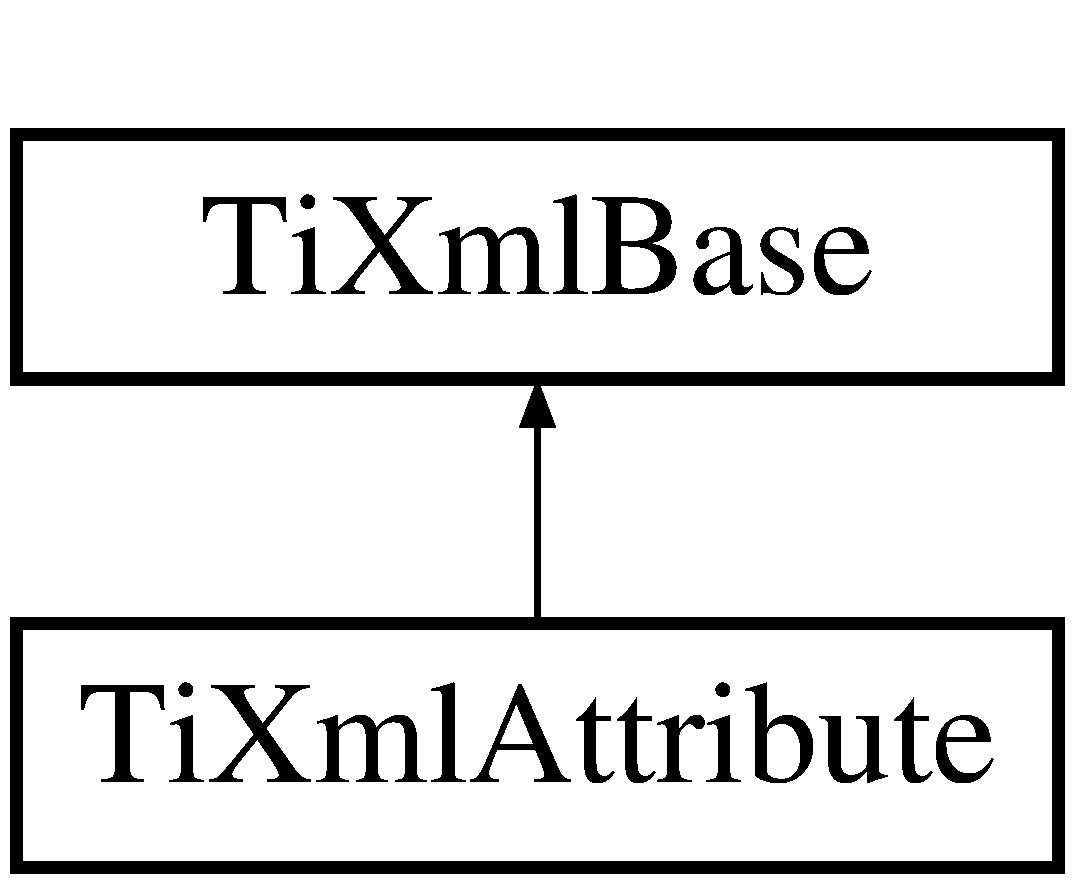
\includegraphics[height=2.000000cm]{class_ti_xml_attribute}
\end{center}
\end{figure}
\subsection*{Public Member Functions}
\begin{DoxyCompactItemize}
\item 
\hypertarget{class_ti_xml_attribute_a9cfa3c8179873fd485d83003b114f8e1}{\hyperlink{class_ti_xml_attribute_a9cfa3c8179873fd485d83003b114f8e1}{Ti\+Xml\+Attribute} ()}\label{class_ti_xml_attribute_a9cfa3c8179873fd485d83003b114f8e1}

\begin{DoxyCompactList}\small\item\em Construct an empty attribute. \end{DoxyCompactList}\item 
\hypertarget{class_ti_xml_attribute_a052213522caac3979960e0714063861d}{\hyperlink{class_ti_xml_attribute_a052213522caac3979960e0714063861d}{Ti\+Xml\+Attribute} (const std\+::string \&\+\_\+name, const std\+::string \&\+\_\+value)}\label{class_ti_xml_attribute_a052213522caac3979960e0714063861d}

\begin{DoxyCompactList}\small\item\em std\+::string constructor. \end{DoxyCompactList}\item 
\hypertarget{class_ti_xml_attribute_a759d0b76fb8fcf765ecab243bc14f05e}{\hyperlink{class_ti_xml_attribute_a759d0b76fb8fcf765ecab243bc14f05e}{Ti\+Xml\+Attribute} (const char $\ast$\+\_\+name, const char $\ast$\+\_\+value)}\label{class_ti_xml_attribute_a759d0b76fb8fcf765ecab243bc14f05e}

\begin{DoxyCompactList}\small\item\em Construct an attribute with a name and value. \end{DoxyCompactList}\item 
\hypertarget{class_ti_xml_attribute_a298a57287d305904ba6bd96ae6f78d3d}{const char $\ast$ \hyperlink{class_ti_xml_attribute_a298a57287d305904ba6bd96ae6f78d3d}{Name} () const }\label{class_ti_xml_attribute_a298a57287d305904ba6bd96ae6f78d3d}

\begin{DoxyCompactList}\small\item\em Return the name of this attribute. \end{DoxyCompactList}\item 
\hypertarget{class_ti_xml_attribute_a0f874490eac8ca00ee0070765d0e97e3}{const char $\ast$ \hyperlink{class_ti_xml_attribute_a0f874490eac8ca00ee0070765d0e97e3}{Value} () const }\label{class_ti_xml_attribute_a0f874490eac8ca00ee0070765d0e97e3}

\begin{DoxyCompactList}\small\item\em Return the value of this attribute. \end{DoxyCompactList}\item 
\hypertarget{class_ti_xml_attribute_a87705c3ccf9ee9417beb4f7cbacd4d33}{const std\+::string \& \hyperlink{class_ti_xml_attribute_a87705c3ccf9ee9417beb4f7cbacd4d33}{Value\+Str} () const }\label{class_ti_xml_attribute_a87705c3ccf9ee9417beb4f7cbacd4d33}

\begin{DoxyCompactList}\small\item\em Return the value of this attribute. \end{DoxyCompactList}\item 
\hypertarget{class_ti_xml_attribute_aa1a20ad59dc7e89a0ab265396360d50f}{int \hyperlink{class_ti_xml_attribute_aa1a20ad59dc7e89a0ab265396360d50f}{Int\+Value} () const }\label{class_ti_xml_attribute_aa1a20ad59dc7e89a0ab265396360d50f}

\begin{DoxyCompactList}\small\item\em Return the value of this attribute, converted to an integer. \end{DoxyCompactList}\item 
\hypertarget{class_ti_xml_attribute_a2880ddef53fc7522c99535273954d230}{double \hyperlink{class_ti_xml_attribute_a2880ddef53fc7522c99535273954d230}{Double\+Value} () const }\label{class_ti_xml_attribute_a2880ddef53fc7522c99535273954d230}

\begin{DoxyCompactList}\small\item\em Return the value of this attribute, converted to a double. \end{DoxyCompactList}\item 
\hypertarget{class_ti_xml_attribute_a64cee17bceb8232eb0736d26dd082d79}{const T\+I\+X\+M\+L\+\_\+\+S\+T\+R\+I\+N\+G \& {\bfseries Name\+T\+Str} () const }\label{class_ti_xml_attribute_a64cee17bceb8232eb0736d26dd082d79}

\item 
int \hyperlink{class_ti_xml_attribute_ad6c93088ee21af41a107931223339344}{Query\+Int\+Value} (int $\ast$\+\_\+value) const 
\item 
\hypertarget{class_ti_xml_attribute_ac87b2a8489906a5d7aa2875f20be3513}{int \hyperlink{class_ti_xml_attribute_ac87b2a8489906a5d7aa2875f20be3513}{Query\+Double\+Value} (double $\ast$\+\_\+value) const }\label{class_ti_xml_attribute_ac87b2a8489906a5d7aa2875f20be3513}

\begin{DoxyCompactList}\small\item\em Query\+Double\+Value examines the value string. See \hyperlink{class_ti_xml_attribute_ad6c93088ee21af41a107931223339344}{Query\+Int\+Value()}. \end{DoxyCompactList}\item 
\hypertarget{class_ti_xml_attribute_ab7fa3d21ff8d7c5764cf9af15b667a99}{void \hyperlink{class_ti_xml_attribute_ab7fa3d21ff8d7c5764cf9af15b667a99}{Set\+Name} (const char $\ast$\+\_\+name)}\label{class_ti_xml_attribute_ab7fa3d21ff8d7c5764cf9af15b667a99}

\begin{DoxyCompactList}\small\item\em Set the name of this attribute. \end{DoxyCompactList}\item 
\hypertarget{class_ti_xml_attribute_a2dae44178f668b3cb48101be4f2236a0}{void \hyperlink{class_ti_xml_attribute_a2dae44178f668b3cb48101be4f2236a0}{Set\+Value} (const char $\ast$\+\_\+value)}\label{class_ti_xml_attribute_a2dae44178f668b3cb48101be4f2236a0}

\begin{DoxyCompactList}\small\item\em Set the value. \end{DoxyCompactList}\item 
\hypertarget{class_ti_xml_attribute_a7e065df640116a62ea4f4b7da5449cc8}{void \hyperlink{class_ti_xml_attribute_a7e065df640116a62ea4f4b7da5449cc8}{Set\+Int\+Value} (int \+\_\+value)}\label{class_ti_xml_attribute_a7e065df640116a62ea4f4b7da5449cc8}

\begin{DoxyCompactList}\small\item\em Set the value from an integer. \end{DoxyCompactList}\item 
\hypertarget{class_ti_xml_attribute_a0316da31373496c4368ad549bf711394}{void \hyperlink{class_ti_xml_attribute_a0316da31373496c4368ad549bf711394}{Set\+Double\+Value} (double \+\_\+value)}\label{class_ti_xml_attribute_a0316da31373496c4368ad549bf711394}

\begin{DoxyCompactList}\small\item\em Set the value from a double. \end{DoxyCompactList}\item 
\hypertarget{class_ti_xml_attribute_ab296ff0c9a8c701055cd257a8a976e57}{void \hyperlink{class_ti_xml_attribute_ab296ff0c9a8c701055cd257a8a976e57}{Set\+Name} (const std\+::string \&\+\_\+name)}\label{class_ti_xml_attribute_ab296ff0c9a8c701055cd257a8a976e57}

\begin{DoxyCompactList}\small\item\em S\+T\+L std\+::string form. \end{DoxyCompactList}\item 
\hypertarget{class_ti_xml_attribute_ab43f67a0cc3ec1d80e62606500f0925f}{void \hyperlink{class_ti_xml_attribute_ab43f67a0cc3ec1d80e62606500f0925f}{Set\+Value} (const std\+::string \&\+\_\+value)}\label{class_ti_xml_attribute_ab43f67a0cc3ec1d80e62606500f0925f}

\begin{DoxyCompactList}\small\item\em S\+T\+L std\+::string form. \end{DoxyCompactList}\item 
\hypertarget{class_ti_xml_attribute_a776478980776a024f7c2846eec640f65}{const \hyperlink{class_ti_xml_attribute}{Ti\+Xml\+Attribute} $\ast$ \hyperlink{class_ti_xml_attribute_a776478980776a024f7c2846eec640f65}{Next} () const }\label{class_ti_xml_attribute_a776478980776a024f7c2846eec640f65}

\begin{DoxyCompactList}\small\item\em Get the next sibling attribute in the D\+O\+M. Returns null at end. \end{DoxyCompactList}\item 
\hypertarget{class_ti_xml_attribute_a138320aa7793b148ba7e5bd0a0ea4db6}{\hyperlink{class_ti_xml_attribute}{Ti\+Xml\+Attribute} $\ast$ {\bfseries Next} ()}\label{class_ti_xml_attribute_a138320aa7793b148ba7e5bd0a0ea4db6}

\item 
\hypertarget{class_ti_xml_attribute_a54a5f8730c7b02b9a41b74e12e27fe86}{const \hyperlink{class_ti_xml_attribute}{Ti\+Xml\+Attribute} $\ast$ \hyperlink{class_ti_xml_attribute_a54a5f8730c7b02b9a41b74e12e27fe86}{Previous} () const }\label{class_ti_xml_attribute_a54a5f8730c7b02b9a41b74e12e27fe86}

\begin{DoxyCompactList}\small\item\em Get the previous sibling attribute in the D\+O\+M. Returns null at beginning. \end{DoxyCompactList}\item 
\hypertarget{class_ti_xml_attribute_ae4dabc932cba945ed1e92fec5f121193}{\hyperlink{class_ti_xml_attribute}{Ti\+Xml\+Attribute} $\ast$ {\bfseries Previous} ()}\label{class_ti_xml_attribute_ae4dabc932cba945ed1e92fec5f121193}

\item 
\hypertarget{class_ti_xml_attribute_ae48c2a65b520d453914ce4e845d607cf}{bool {\bfseries operator==} (const \hyperlink{class_ti_xml_attribute}{Ti\+Xml\+Attribute} \&rhs) const }\label{class_ti_xml_attribute_ae48c2a65b520d453914ce4e845d607cf}

\item 
\hypertarget{class_ti_xml_attribute_adb8b6f2cad5948e73e383182e7ce10de}{bool {\bfseries operator$<$} (const \hyperlink{class_ti_xml_attribute}{Ti\+Xml\+Attribute} \&rhs) const }\label{class_ti_xml_attribute_adb8b6f2cad5948e73e383182e7ce10de}

\item 
\hypertarget{class_ti_xml_attribute_a867562769ef9778c1690cd373246b05b}{bool {\bfseries operator$>$} (const \hyperlink{class_ti_xml_attribute}{Ti\+Xml\+Attribute} \&rhs) const }\label{class_ti_xml_attribute_a867562769ef9778c1690cd373246b05b}

\item 
\hypertarget{class_ti_xml_attribute_ad62774421b814894b995af3b5d231dda}{virtual const char $\ast$ {\bfseries Parse} (const char $\ast$p, \hyperlink{class_ti_xml_parsing_data}{Ti\+Xml\+Parsing\+Data} $\ast$data, Ti\+Xml\+Encoding encoding)}\label{class_ti_xml_attribute_ad62774421b814894b995af3b5d231dda}

\item 
virtual void \hyperlink{class_ti_xml_attribute_acc04956c1d5c4c31fe74f7a7528d109a}{Print} (F\+I\+L\+E $\ast$cfile, int depth) const 
\item 
\hypertarget{class_ti_xml_attribute_a19e6b6862a80b188571c47947e88d030}{void {\bfseries Print} (F\+I\+L\+E $\ast$cfile, int depth, T\+I\+X\+M\+L\+\_\+\+S\+T\+R\+I\+N\+G $\ast$str) const }\label{class_ti_xml_attribute_a19e6b6862a80b188571c47947e88d030}

\item 
\hypertarget{class_ti_xml_attribute_ac12a94d4548302afb12f488ba101f7d1}{void {\bfseries Set\+Document} (\hyperlink{class_ti_xml_document}{Ti\+Xml\+Document} $\ast$doc)}\label{class_ti_xml_attribute_ac12a94d4548302afb12f488ba101f7d1}

\end{DoxyCompactItemize}
\subsection*{Friends}
\begin{DoxyCompactItemize}
\item 
\hypertarget{class_ti_xml_attribute_a35a7b7f89f708527677d5078d41ce0bf}{class {\bfseries Ti\+Xml\+Attribute\+Set}}\label{class_ti_xml_attribute_a35a7b7f89f708527677d5078d41ce0bf}

\end{DoxyCompactItemize}
\subsection*{Additional Inherited Members}


\subsection{Detailed Description}
An attribute is a name-\/value pair. Elements have an arbitrary number of attributes, each with a unique name.

\begin{DoxyNote}{Note}
The attributes are not Ti\+Xml\+Nodes, since they are not part of the tiny\+X\+M\+L document object model. There are other suggested ways to look at this problem. 
\end{DoxyNote}


\subsection{Member Function Documentation}
\hypertarget{class_ti_xml_attribute_acc04956c1d5c4c31fe74f7a7528d109a}{\index{Ti\+Xml\+Attribute@{Ti\+Xml\+Attribute}!Print@{Print}}
\index{Print@{Print}!Ti\+Xml\+Attribute@{Ti\+Xml\+Attribute}}
\subsubsection[{Print}]{\setlength{\rightskip}{0pt plus 5cm}virtual void Ti\+Xml\+Attribute\+::\+Print (
\begin{DoxyParamCaption}
\item[{F\+I\+L\+E $\ast$}]{cfile, }
\item[{int}]{depth}
\end{DoxyParamCaption}
) const\hspace{0.3cm}{\ttfamily [inline]}, {\ttfamily [virtual]}}}\label{class_ti_xml_attribute_acc04956c1d5c4c31fe74f7a7528d109a}
All Tiny\+Xml classes can print themselves to a filestream or the string class (\hyperlink{class_ti_xml_string}{Ti\+Xml\+String} in non-\/\+S\+T\+L mode, std\+::string in S\+T\+L mode.) Either or both cfile and str can be null.

This is a formatted print, and will insert tabs and newlines.

(For an unformatted stream, use the $<$$<$ operator.) 

Implements \hyperlink{class_ti_xml_base_a0de56b3f2ef14c65091a3b916437b512}{Ti\+Xml\+Base}.

\hypertarget{class_ti_xml_attribute_ad6c93088ee21af41a107931223339344}{\index{Ti\+Xml\+Attribute@{Ti\+Xml\+Attribute}!Query\+Int\+Value@{Query\+Int\+Value}}
\index{Query\+Int\+Value@{Query\+Int\+Value}!Ti\+Xml\+Attribute@{Ti\+Xml\+Attribute}}
\subsubsection[{Query\+Int\+Value}]{\setlength{\rightskip}{0pt plus 5cm}int Ti\+Xml\+Attribute\+::\+Query\+Int\+Value (
\begin{DoxyParamCaption}
\item[{int $\ast$}]{\+\_\+value}
\end{DoxyParamCaption}
) const}}\label{class_ti_xml_attribute_ad6c93088ee21af41a107931223339344}
Query\+Int\+Value examines the value string. It is an alternative to the \hyperlink{class_ti_xml_attribute_aa1a20ad59dc7e89a0ab265396360d50f}{Int\+Value()} method with richer error checking. If the value is an integer, it is stored in 'value' and the call returns T\+I\+X\+M\+L\+\_\+\+S\+U\+C\+C\+E\+S\+S. If it is not an integer, it returns T\+I\+X\+M\+L\+\_\+\+W\+R\+O\+N\+G\+\_\+\+T\+Y\+P\+E.

A specialized but useful call. Note that for success it returns 0, which is the opposite of almost all other Tiny\+Xml calls. 

The documentation for this class was generated from the following files\+:\begin{DoxyCompactItemize}
\item 
C\+:/\+Users/\+Avenger/\+Documents/\+Git\+Hub/\+Projet-\/\+Tamagoshi/includes/tinyxml/tinyxml.\+h\item 
C\+:/\+Users/\+Avenger/\+Documents/\+Git\+Hub/\+Projet-\/\+Tamagoshi/includes/tinyxml/tinyxml.\+cpp\item 
C\+:/\+Users/\+Avenger/\+Documents/\+Git\+Hub/\+Projet-\/\+Tamagoshi/includes/tinyxml/tinyxmlparser.\+cpp\end{DoxyCompactItemize}

\hypertarget{class_ti_xml_attribute_set}{\section{Ti\+Xml\+Attribute\+Set Class Reference}
\label{class_ti_xml_attribute_set}\index{Ti\+Xml\+Attribute\+Set@{Ti\+Xml\+Attribute\+Set}}
}
\subsection*{Public Member Functions}
\begin{DoxyCompactItemize}
\item 
\hypertarget{class_ti_xml_attribute_set_a745e50ddaae3bee93e4589321e0b9c1a}{void {\bfseries Add} (\hyperlink{class_ti_xml_attribute}{Ti\+Xml\+Attribute} $\ast$attribute)}\label{class_ti_xml_attribute_set_a745e50ddaae3bee93e4589321e0b9c1a}

\item 
\hypertarget{class_ti_xml_attribute_set_a924a73d071f2573f9060f0be57879c57}{void {\bfseries Remove} (\hyperlink{class_ti_xml_attribute}{Ti\+Xml\+Attribute} $\ast$attribute)}\label{class_ti_xml_attribute_set_a924a73d071f2573f9060f0be57879c57}

\item 
\hypertarget{class_ti_xml_attribute_set_ae0636e88cedd4b09d61c451860f68598}{const \hyperlink{class_ti_xml_attribute}{Ti\+Xml\+Attribute} $\ast$ {\bfseries First} () const }\label{class_ti_xml_attribute_set_ae0636e88cedd4b09d61c451860f68598}

\item 
\hypertarget{class_ti_xml_attribute_set_a99703bb08ca2aece2d7ef835de339ba0}{\hyperlink{class_ti_xml_attribute}{Ti\+Xml\+Attribute} $\ast$ {\bfseries First} ()}\label{class_ti_xml_attribute_set_a99703bb08ca2aece2d7ef835de339ba0}

\item 
\hypertarget{class_ti_xml_attribute_set_a7b3f3ccf39a97bc25539d3fcc540296a}{const \hyperlink{class_ti_xml_attribute}{Ti\+Xml\+Attribute} $\ast$ {\bfseries Last} () const }\label{class_ti_xml_attribute_set_a7b3f3ccf39a97bc25539d3fcc540296a}

\item 
\hypertarget{class_ti_xml_attribute_set_ab4c4edfb2d74f6ea31aae096743bd6e0}{\hyperlink{class_ti_xml_attribute}{Ti\+Xml\+Attribute} $\ast$ {\bfseries Last} ()}\label{class_ti_xml_attribute_set_ab4c4edfb2d74f6ea31aae096743bd6e0}

\item 
\hypertarget{class_ti_xml_attribute_set_af3675cc2bfd0aea153cda1cfcdd1f77e}{\hyperlink{class_ti_xml_attribute}{Ti\+Xml\+Attribute} $\ast$ {\bfseries Find} (const char $\ast$\+\_\+name) const }\label{class_ti_xml_attribute_set_af3675cc2bfd0aea153cda1cfcdd1f77e}

\item 
\hypertarget{class_ti_xml_attribute_set_a5e28f5d32f048fba85d04dc317495bdc}{\hyperlink{class_ti_xml_attribute}{Ti\+Xml\+Attribute} $\ast$ {\bfseries Find\+Or\+Create} (const char $\ast$\+\_\+name)}\label{class_ti_xml_attribute_set_a5e28f5d32f048fba85d04dc317495bdc}

\item 
\hypertarget{class_ti_xml_attribute_set_ab6d6c98b99a257e38fec81cae36a54d1}{\hyperlink{class_ti_xml_attribute}{Ti\+Xml\+Attribute} $\ast$ {\bfseries Find} (const std\+::string \&\+\_\+name) const }\label{class_ti_xml_attribute_set_ab6d6c98b99a257e38fec81cae36a54d1}

\item 
\hypertarget{class_ti_xml_attribute_set_acccd76e3d87a92caed2795266c6e540e}{\hyperlink{class_ti_xml_attribute}{Ti\+Xml\+Attribute} $\ast$ {\bfseries Find\+Or\+Create} (const std\+::string \&\+\_\+name)}\label{class_ti_xml_attribute_set_acccd76e3d87a92caed2795266c6e540e}

\end{DoxyCompactItemize}


The documentation for this class was generated from the following files\+:\begin{DoxyCompactItemize}
\item 
C\+:/\+Users/\+Avenger/\+Documents/\+Git\+Hub/\+Projet-\/\+Tamagoshi/includes/tinyxml/tinyxml.\+h\item 
C\+:/\+Users/\+Avenger/\+Documents/\+Git\+Hub/\+Projet-\/\+Tamagoshi/includes/tinyxml/tinyxml.\+cpp\end{DoxyCompactItemize}

\hypertarget{class_ti_xml_base}{\section{Ti\+Xml\+Base Class Reference}
\label{class_ti_xml_base}\index{Ti\+Xml\+Base@{Ti\+Xml\+Base}}
}


{\ttfamily \#include $<$tinyxml.\+h$>$}

Inheritance diagram for Ti\+Xml\+Base\+:\begin{figure}[H]
\begin{center}
\leavevmode
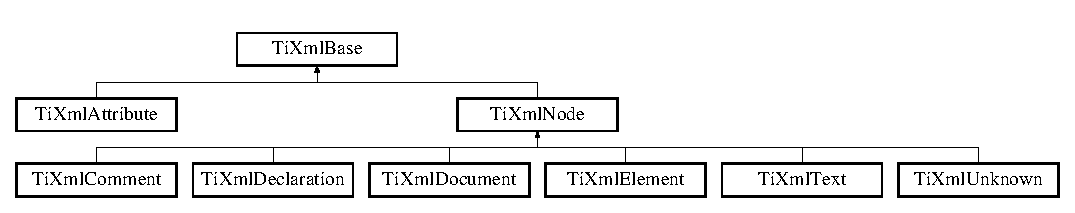
\includegraphics[height=2.413793cm]{class_ti_xml_base}
\end{center}
\end{figure}
\subsection*{Public Types}
\begin{DoxyCompactItemize}
\item 
\hypertarget{class_ti_xml_base_a9a7e9344415956ab96e8c75f6a0bbd48}{enum \{ \\*
{\bfseries T\+I\+X\+M\+L\+\_\+\+N\+O\+\_\+\+E\+R\+R\+O\+R} = 0, 
{\bfseries T\+I\+X\+M\+L\+\_\+\+E\+R\+R\+O\+R}, 
{\bfseries T\+I\+X\+M\+L\+\_\+\+E\+R\+R\+O\+R\+\_\+\+O\+P\+E\+N\+I\+N\+G\+\_\+\+F\+I\+L\+E}, 
{\bfseries T\+I\+X\+M\+L\+\_\+\+E\+R\+R\+O\+R\+\_\+\+P\+A\+R\+S\+I\+N\+G\+\_\+\+E\+L\+E\+M\+E\+N\+T}, 
\\*
{\bfseries T\+I\+X\+M\+L\+\_\+\+E\+R\+R\+O\+R\+\_\+\+F\+A\+I\+L\+E\+D\+\_\+\+T\+O\+\_\+\+R\+E\+A\+D\+\_\+\+E\+L\+E\+M\+E\+N\+T\+\_\+\+N\+A\+M\+E}, 
{\bfseries T\+I\+X\+M\+L\+\_\+\+E\+R\+R\+O\+R\+\_\+\+R\+E\+A\+D\+I\+N\+G\+\_\+\+E\+L\+E\+M\+E\+N\+T\+\_\+\+V\+A\+L\+U\+E}, 
{\bfseries T\+I\+X\+M\+L\+\_\+\+E\+R\+R\+O\+R\+\_\+\+R\+E\+A\+D\+I\+N\+G\+\_\+\+A\+T\+T\+R\+I\+B\+U\+T\+E\+S}, 
{\bfseries T\+I\+X\+M\+L\+\_\+\+E\+R\+R\+O\+R\+\_\+\+P\+A\+R\+S\+I\+N\+G\+\_\+\+E\+M\+P\+T\+Y}, 
\\*
{\bfseries T\+I\+X\+M\+L\+\_\+\+E\+R\+R\+O\+R\+\_\+\+R\+E\+A\+D\+I\+N\+G\+\_\+\+E\+N\+D\+\_\+\+T\+A\+G}, 
{\bfseries T\+I\+X\+M\+L\+\_\+\+E\+R\+R\+O\+R\+\_\+\+P\+A\+R\+S\+I\+N\+G\+\_\+\+U\+N\+K\+N\+O\+W\+N}, 
{\bfseries T\+I\+X\+M\+L\+\_\+\+E\+R\+R\+O\+R\+\_\+\+P\+A\+R\+S\+I\+N\+G\+\_\+\+C\+O\+M\+M\+E\+N\+T}, 
{\bfseries T\+I\+X\+M\+L\+\_\+\+E\+R\+R\+O\+R\+\_\+\+P\+A\+R\+S\+I\+N\+G\+\_\+\+D\+E\+C\+L\+A\+R\+A\+T\+I\+O\+N}, 
\\*
{\bfseries T\+I\+X\+M\+L\+\_\+\+E\+R\+R\+O\+R\+\_\+\+D\+O\+C\+U\+M\+E\+N\+T\+\_\+\+E\+M\+P\+T\+Y}, 
{\bfseries T\+I\+X\+M\+L\+\_\+\+E\+R\+R\+O\+R\+\_\+\+E\+M\+B\+E\+D\+D\+E\+D\+\_\+\+N\+U\+L\+L}, 
{\bfseries T\+I\+X\+M\+L\+\_\+\+E\+R\+R\+O\+R\+\_\+\+P\+A\+R\+S\+I\+N\+G\+\_\+\+C\+D\+A\+T\+A}, 
{\bfseries T\+I\+X\+M\+L\+\_\+\+E\+R\+R\+O\+R\+\_\+\+D\+O\+C\+U\+M\+E\+N\+T\+\_\+\+T\+O\+P\+\_\+\+O\+N\+L\+Y}, 
\\*
{\bfseries T\+I\+X\+M\+L\+\_\+\+E\+R\+R\+O\+R\+\_\+\+S\+T\+R\+I\+N\+G\+\_\+\+C\+O\+U\+N\+T}
 \}}\label{class_ti_xml_base_a9a7e9344415956ab96e8c75f6a0bbd48}

\end{DoxyCompactItemize}
\subsection*{Public Member Functions}
\begin{DoxyCompactItemize}
\item 
virtual void \hyperlink{class_ti_xml_base_a0de56b3f2ef14c65091a3b916437b512}{Print} (F\+I\+L\+E $\ast$cfile, int depth) const =0
\item 
int \hyperlink{class_ti_xml_base_a024bceb070188df92c2a8d8852dd0853}{Row} () const 
\item 
\hypertarget{class_ti_xml_base_ab54bfb9b70fe6dd276e7b279cab7f003}{int \hyperlink{class_ti_xml_base_ab54bfb9b70fe6dd276e7b279cab7f003}{Column} () const }\label{class_ti_xml_base_ab54bfb9b70fe6dd276e7b279cab7f003}

\begin{DoxyCompactList}\small\item\em See \hyperlink{class_ti_xml_base_a024bceb070188df92c2a8d8852dd0853}{Row()} \end{DoxyCompactList}\item 
\hypertarget{class_ti_xml_base_ac6b3e0f790930d4970ec30764e937b5d}{void \hyperlink{class_ti_xml_base_ac6b3e0f790930d4970ec30764e937b5d}{Set\+User\+Data} (void $\ast$user)}\label{class_ti_xml_base_ac6b3e0f790930d4970ec30764e937b5d}

\begin{DoxyCompactList}\small\item\em Set a pointer to arbitrary user data. \end{DoxyCompactList}\item 
\hypertarget{class_ti_xml_base_a6559a530ca6763fc301a14d77ed28c17}{void $\ast$ \hyperlink{class_ti_xml_base_a6559a530ca6763fc301a14d77ed28c17}{Get\+User\+Data} ()}\label{class_ti_xml_base_a6559a530ca6763fc301a14d77ed28c17}

\begin{DoxyCompactList}\small\item\em Get a pointer to arbitrary user data. \end{DoxyCompactList}\item 
\hypertarget{class_ti_xml_base_ad0120210e4680ef2088601753ce0ede4}{const void $\ast$ \hyperlink{class_ti_xml_base_ad0120210e4680ef2088601753ce0ede4}{Get\+User\+Data} () const }\label{class_ti_xml_base_ad0120210e4680ef2088601753ce0ede4}

\begin{DoxyCompactList}\small\item\em Get a pointer to arbitrary user data. \end{DoxyCompactList}\item 
\hypertarget{class_ti_xml_base_a00e4edb0219d00a1379c856e5a1d2025}{virtual const char $\ast$ {\bfseries Parse} (const char $\ast$p, \hyperlink{class_ti_xml_parsing_data}{Ti\+Xml\+Parsing\+Data} $\ast$data, Ti\+Xml\+Encoding encoding)=0}\label{class_ti_xml_base_a00e4edb0219d00a1379c856e5a1d2025}

\end{DoxyCompactItemize}
\subsection*{Static Public Member Functions}
\begin{DoxyCompactItemize}
\item 
static void \hyperlink{class_ti_xml_base_a0f799ec645bfb8d8a969e83478f379c1}{Set\+Condense\+White\+Space} (bool condense)
\item 
\hypertarget{class_ti_xml_base_ad4b1472531c647a25b1840a87ae42438}{static bool \hyperlink{class_ti_xml_base_ad4b1472531c647a25b1840a87ae42438}{Is\+White\+Space\+Condensed} ()}\label{class_ti_xml_base_ad4b1472531c647a25b1840a87ae42438}

\begin{DoxyCompactList}\small\item\em Return the current white space setting. \end{DoxyCompactList}\item 
static void \hyperlink{class_ti_xml_base_a32ed202562b58de64c7d799ca3c9db98}{Encode\+String} (const T\+I\+X\+M\+L\+\_\+\+S\+T\+R\+I\+N\+G \&str, T\+I\+X\+M\+L\+\_\+\+S\+T\+R\+I\+N\+G $\ast$out)
\end{DoxyCompactItemize}
\subsection*{Static Public Attributes}
\begin{DoxyCompactItemize}
\item 
static const int {\bfseries utf8\+Byte\+Table} \mbox{[}256\mbox{]}
\end{DoxyCompactItemize}
\subsection*{Static Protected Member Functions}
\begin{DoxyCompactItemize}
\item 
\hypertarget{class_ti_xml_base_ac0c3d66d8a9e6996a1fa016275e16875}{static const char $\ast$ {\bfseries Skip\+White\+Space} (const char $\ast$, Ti\+Xml\+Encoding encoding)}\label{class_ti_xml_base_ac0c3d66d8a9e6996a1fa016275e16875}

\item 
\hypertarget{class_ti_xml_base_af56296d561c0bab4bc8e198cdcf5c48e}{static bool {\bfseries Is\+White\+Space} (char c)}\label{class_ti_xml_base_af56296d561c0bab4bc8e198cdcf5c48e}

\item 
\hypertarget{class_ti_xml_base_a3de391ea9f4c4a8aa10d04480b048795}{static bool {\bfseries Is\+White\+Space} (int c)}\label{class_ti_xml_base_a3de391ea9f4c4a8aa10d04480b048795}

\item 
\hypertarget{class_ti_xml_base_a189eaa418ff6628bdabf4bf8fb1bd633}{static bool {\bfseries Stream\+White\+Space} (std\+::istream $\ast$in, T\+I\+X\+M\+L\+\_\+\+S\+T\+R\+I\+N\+G $\ast$tag)}\label{class_ti_xml_base_a189eaa418ff6628bdabf4bf8fb1bd633}

\item 
\hypertarget{class_ti_xml_base_aae465f424a9bcf7a9cf2426c62da8e6b}{static bool {\bfseries Stream\+To} (std\+::istream $\ast$in, int character, T\+I\+X\+M\+L\+\_\+\+S\+T\+R\+I\+N\+G $\ast$tag)}\label{class_ti_xml_base_aae465f424a9bcf7a9cf2426c62da8e6b}

\item 
\hypertarget{class_ti_xml_base_a1c21a6ab5f7b503acd91f35f183734b3}{static const char $\ast$ {\bfseries Read\+Name} (const char $\ast$p, T\+I\+X\+M\+L\+\_\+\+S\+T\+R\+I\+N\+G $\ast$name, Ti\+Xml\+Encoding encoding)}\label{class_ti_xml_base_a1c21a6ab5f7b503acd91f35f183734b3}

\item 
\hypertarget{class_ti_xml_base_aa646c74921aa33156968b802bbf5566e}{static const char $\ast$ {\bfseries Read\+Text} (const char $\ast$in, T\+I\+X\+M\+L\+\_\+\+S\+T\+R\+I\+N\+G $\ast$text, bool ignore\+White\+Space, const char $\ast$end\+Tag, bool ignore\+Case, Ti\+Xml\+Encoding encoding)}\label{class_ti_xml_base_aa646c74921aa33156968b802bbf5566e}

\item 
\hypertarget{class_ti_xml_base_ac5c08bf3deffcda0bf8ce2958372b584}{static const char $\ast$ {\bfseries Get\+Entity} (const char $\ast$in, char $\ast$value, int $\ast$length, Ti\+Xml\+Encoding encoding)}\label{class_ti_xml_base_ac5c08bf3deffcda0bf8ce2958372b584}

\item 
\hypertarget{class_ti_xml_base_a5b0fde72d6f662ae1fd6303195d2159b}{static const char $\ast$ {\bfseries Get\+Char} (const char $\ast$p, char $\ast$\+\_\+value, int $\ast$length, Ti\+Xml\+Encoding encoding)}\label{class_ti_xml_base_a5b0fde72d6f662ae1fd6303195d2159b}

\item 
\hypertarget{class_ti_xml_base_a51631e6986179558b9e5850723ed165a}{static bool {\bfseries String\+Equal} (const char $\ast$p, const char $\ast$end\+Tag, bool ignore\+Case, Ti\+Xml\+Encoding encoding)}\label{class_ti_xml_base_a51631e6986179558b9e5850723ed165a}

\item 
\hypertarget{class_ti_xml_base_ae22522b2e8e1ac43102d16394f639fc8}{static int {\bfseries Is\+Alpha} (unsigned char any\+Byte, Ti\+Xml\+Encoding encoding)}\label{class_ti_xml_base_ae22522b2e8e1ac43102d16394f639fc8}

\item 
\hypertarget{class_ti_xml_base_a321919055c115c78ded17f85a793f368}{static int {\bfseries Is\+Alpha\+Num} (unsigned char any\+Byte, Ti\+Xml\+Encoding encoding)}\label{class_ti_xml_base_a321919055c115c78ded17f85a793f368}

\item 
\hypertarget{class_ti_xml_base_a799f17405a86a5c2029618e85f11a097}{static int {\bfseries To\+Lower} (int v, Ti\+Xml\+Encoding encoding)}\label{class_ti_xml_base_a799f17405a86a5c2029618e85f11a097}

\item 
\hypertarget{class_ti_xml_base_a07c765e3a7f979d343e646ea797b180b}{static void {\bfseries Convert\+U\+T\+F32\+To\+U\+T\+F8} (unsigned long input, char $\ast$output, int $\ast$length)}\label{class_ti_xml_base_a07c765e3a7f979d343e646ea797b180b}

\end{DoxyCompactItemize}
\subsection*{Protected Attributes}
\begin{DoxyCompactItemize}
\item 
\hypertarget{class_ti_xml_base_a0d992580f3bc264909f898e942677a3c}{\hyperlink{struct_ti_xml_cursor}{Ti\+Xml\+Cursor} {\bfseries location}}\label{class_ti_xml_base_a0d992580f3bc264909f898e942677a3c}

\item 
\hypertarget{class_ti_xml_base_ab242c01590191f644569fa89a080d97c}{void $\ast$ \hyperlink{class_ti_xml_base_ab242c01590191f644569fa89a080d97c}{user\+Data}}\label{class_ti_xml_base_ab242c01590191f644569fa89a080d97c}

\begin{DoxyCompactList}\small\item\em Field containing a generic user pointer. \end{DoxyCompactList}\end{DoxyCompactItemize}
\subsection*{Static Protected Attributes}
\begin{DoxyCompactItemize}
\item 
static const char $\ast$ {\bfseries error\+String} \mbox{[}T\+I\+X\+M\+L\+\_\+\+E\+R\+R\+O\+R\+\_\+\+S\+T\+R\+I\+N\+G\+\_\+\+C\+O\+U\+N\+T\mbox{]}
\end{DoxyCompactItemize}
\subsection*{Friends}
\begin{DoxyCompactItemize}
\item 
\hypertarget{class_ti_xml_base_a218872a0d985ae30e78c55adc4bdb196}{class {\bfseries Ti\+Xml\+Node}}\label{class_ti_xml_base_a218872a0d985ae30e78c55adc4bdb196}

\item 
\hypertarget{class_ti_xml_base_ab6592e32cb9132be517cc12a70564c4b}{class {\bfseries Ti\+Xml\+Element}}\label{class_ti_xml_base_ab6592e32cb9132be517cc12a70564c4b}

\item 
\hypertarget{class_ti_xml_base_a173617f6dfe902cf484ce5552b950475}{class {\bfseries Ti\+Xml\+Document}}\label{class_ti_xml_base_a173617f6dfe902cf484ce5552b950475}

\end{DoxyCompactItemize}


\subsection{Detailed Description}
\hyperlink{class_ti_xml_base}{Ti\+Xml\+Base} is a base class for every class in Tiny\+Xml. It does little except to establish that Tiny\+Xml classes can be printed and provide some utility functions.

In X\+M\+L, the document and elements can contain other elements and other types of nodes.

\begin{DoxyVerb}A Document can contain: Element (container or leaf)
                        Comment (leaf)
                        Unknown (leaf)
                        Declaration( leaf )

An Element can contain: Element (container or leaf)
                        Text    (leaf)
                        Attributes (not on tree)
                        Comment (leaf)
                        Unknown (leaf)

A Decleration contains: Attributes (not on tree)
\end{DoxyVerb}
 

\subsection{Member Function Documentation}
\hypertarget{class_ti_xml_base_a32ed202562b58de64c7d799ca3c9db98}{\index{Ti\+Xml\+Base@{Ti\+Xml\+Base}!Encode\+String@{Encode\+String}}
\index{Encode\+String@{Encode\+String}!Ti\+Xml\+Base@{Ti\+Xml\+Base}}
\subsubsection[{Encode\+String}]{\setlength{\rightskip}{0pt plus 5cm}void Ti\+Xml\+Base\+::\+Encode\+String (
\begin{DoxyParamCaption}
\item[{const T\+I\+X\+M\+L\+\_\+\+S\+T\+R\+I\+N\+G \&}]{str, }
\item[{T\+I\+X\+M\+L\+\_\+\+S\+T\+R\+I\+N\+G $\ast$}]{out}
\end{DoxyParamCaption}
)\hspace{0.3cm}{\ttfamily [static]}}}\label{class_ti_xml_base_a32ed202562b58de64c7d799ca3c9db98}
Expands entities in a string. Note this should not contian the tag's '$<$', '$>$', etc, or they will be transformed into entities! \hypertarget{class_ti_xml_base_a0de56b3f2ef14c65091a3b916437b512}{\index{Ti\+Xml\+Base@{Ti\+Xml\+Base}!Print@{Print}}
\index{Print@{Print}!Ti\+Xml\+Base@{Ti\+Xml\+Base}}
\subsubsection[{Print}]{\setlength{\rightskip}{0pt plus 5cm}virtual void Ti\+Xml\+Base\+::\+Print (
\begin{DoxyParamCaption}
\item[{F\+I\+L\+E $\ast$}]{cfile, }
\item[{int}]{depth}
\end{DoxyParamCaption}
) const\hspace{0.3cm}{\ttfamily [pure virtual]}}}\label{class_ti_xml_base_a0de56b3f2ef14c65091a3b916437b512}
All Tiny\+Xml classes can print themselves to a filestream or the string class (\hyperlink{class_ti_xml_string}{Ti\+Xml\+String} in non-\/\+S\+T\+L mode, std\+::string in S\+T\+L mode.) Either or both cfile and str can be null.

This is a formatted print, and will insert tabs and newlines.

(For an unformatted stream, use the $<$$<$ operator.) 

Implemented in \hyperlink{class_ti_xml_document_a7b1aea204fee266b70b9c105c8bf2ada}{Ti\+Xml\+Document}, \hyperlink{class_ti_xml_unknown_a025f19c21ef01ea9be50febb8fe0ba06}{Ti\+Xml\+Unknown}, \hyperlink{class_ti_xml_declaration_abf6303db4bd05b5be554036817ff1cb4}{Ti\+Xml\+Declaration}, \hyperlink{class_ti_xml_text_ae74d56c5b3ddec6cc3103dd51821af92}{Ti\+Xml\+Text}, \hyperlink{class_ti_xml_comment_a17398061d62c470f57801ce28fa33ad4}{Ti\+Xml\+Comment}, \hyperlink{class_ti_xml_element_ad9d0c008866982ab8d9aafae7e14d692}{Ti\+Xml\+Element}, and \hyperlink{class_ti_xml_attribute_acc04956c1d5c4c31fe74f7a7528d109a}{Ti\+Xml\+Attribute}.

\hypertarget{class_ti_xml_base_a024bceb070188df92c2a8d8852dd0853}{\index{Ti\+Xml\+Base@{Ti\+Xml\+Base}!Row@{Row}}
\index{Row@{Row}!Ti\+Xml\+Base@{Ti\+Xml\+Base}}
\subsubsection[{Row}]{\setlength{\rightskip}{0pt plus 5cm}int Ti\+Xml\+Base\+::\+Row (
\begin{DoxyParamCaption}
{}
\end{DoxyParamCaption}
) const\hspace{0.3cm}{\ttfamily [inline]}}}\label{class_ti_xml_base_a024bceb070188df92c2a8d8852dd0853}
Return the position, in the original source file, of this node or attribute. The row and column are 1-\/based. (That is the first row and first column is 1,1). If the returns values are 0 or less, then the parser does not have a row and column value.

Generally, the row and column value will be set when the Ti\+Xml\+Document\+::\+Load(), \hyperlink{class_ti_xml_document_a4c852a889c02cf251117fd1d9fe1845f}{Ti\+Xml\+Document\+::\+Load\+File()}, or any Ti\+Xml\+Node\+::\+Parse() is called. It will N\+O\+T be set when the D\+O\+M was created from operator$>$$>$.

The values reflect the initial load. Once the D\+O\+M is modified programmatically (by adding or changing nodes and attributes) the new values will N\+O\+T update to reflect changes in the document.

There is a minor performance cost to computing the row and column. Computation can be disabled if \hyperlink{class_ti_xml_document_a51dac56316f89b35bdb7d0d433ba988e}{Ti\+Xml\+Document\+::\+Set\+Tab\+Size()} is called with 0 as the value.

\begin{DoxySeeAlso}{See also}
\hyperlink{class_ti_xml_document_a51dac56316f89b35bdb7d0d433ba988e}{Ti\+Xml\+Document\+::\+Set\+Tab\+Size()} 
\end{DoxySeeAlso}
\hypertarget{class_ti_xml_base_a0f799ec645bfb8d8a969e83478f379c1}{\index{Ti\+Xml\+Base@{Ti\+Xml\+Base}!Set\+Condense\+White\+Space@{Set\+Condense\+White\+Space}}
\index{Set\+Condense\+White\+Space@{Set\+Condense\+White\+Space}!Ti\+Xml\+Base@{Ti\+Xml\+Base}}
\subsubsection[{Set\+Condense\+White\+Space}]{\setlength{\rightskip}{0pt plus 5cm}static void Ti\+Xml\+Base\+::\+Set\+Condense\+White\+Space (
\begin{DoxyParamCaption}
\item[{bool}]{condense}
\end{DoxyParamCaption}
)\hspace{0.3cm}{\ttfamily [inline]}, {\ttfamily [static]}}}\label{class_ti_xml_base_a0f799ec645bfb8d8a969e83478f379c1}
The world does not agree on whether white space should be kept or not. In order to make everyone happy, these global, static functions are provided to set whether or not Tiny\+Xml will condense all white space into a single space or not. The default is to condense. Note changing this value is not thread safe. 

\subsection{Member Data Documentation}
\hypertarget{class_ti_xml_base_a7ac8feec4100e446b3d78e1ac0659700}{\index{Ti\+Xml\+Base@{Ti\+Xml\+Base}!error\+String@{error\+String}}
\index{error\+String@{error\+String}!Ti\+Xml\+Base@{Ti\+Xml\+Base}}
\subsubsection[{error\+String}]{\setlength{\rightskip}{0pt plus 5cm}const char $\ast$ Ti\+Xml\+Base\+::error\+String\hspace{0.3cm}{\ttfamily [static]}, {\ttfamily [protected]}}}\label{class_ti_xml_base_a7ac8feec4100e446b3d78e1ac0659700}
{\bfseries Initial value\+:}
\begin{DoxyCode}
=
\{
    \textcolor{stringliteral}{"No error"},
    \textcolor{stringliteral}{"Error"},
    \textcolor{stringliteral}{"Failed to open file"},
    \textcolor{stringliteral}{"Error parsing Element."},
    \textcolor{stringliteral}{"Failed to read Element name"},
    \textcolor{stringliteral}{"Error reading Element value."},
    \textcolor{stringliteral}{"Error reading Attributes."},
    \textcolor{stringliteral}{"Error: empty tag."},
    \textcolor{stringliteral}{"Error reading end tag."},
    \textcolor{stringliteral}{"Error parsing Unknown."},
    \textcolor{stringliteral}{"Error parsing Comment."},
    \textcolor{stringliteral}{"Error parsing Declaration."},
    \textcolor{stringliteral}{"Error document empty."},
    \textcolor{stringliteral}{"Error null (0) or unexpected EOF found in input stream."},
    \textcolor{stringliteral}{"Error parsing CDATA."},
    \textcolor{stringliteral}{"Error when TiXmlDocument added to document, because TiXmlDocument can only be at the root."},
\}
\end{DoxyCode}
\hypertarget{class_ti_xml_base_ac8c86058137bdb4b413c3eca58f2d467}{\index{Ti\+Xml\+Base@{Ti\+Xml\+Base}!utf8\+Byte\+Table@{utf8\+Byte\+Table}}
\index{utf8\+Byte\+Table@{utf8\+Byte\+Table}!Ti\+Xml\+Base@{Ti\+Xml\+Base}}
\subsubsection[{utf8\+Byte\+Table}]{\setlength{\rightskip}{0pt plus 5cm}const int Ti\+Xml\+Base\+::utf8\+Byte\+Table\hspace{0.3cm}{\ttfamily [static]}}}\label{class_ti_xml_base_ac8c86058137bdb4b413c3eca58f2d467}
{\bfseries Initial value\+:}
\begin{DoxyCode}
= 
\{
    
        1,  1,  1,  1,  1,  1,  1,  1,  1,  1,  1,  1,  1,  1,  1,  1,  
        1,  1,  1,  1,  1,  1,  1,  1,  1,  1,  1,  1,  1,  1,  1,  1,  
        1,  1,  1,  1,  1,  1,  1,  1,  1,  1,  1,  1,  1,  1,  1,  1,  
        1,  1,  1,  1,  1,  1,  1,  1,  1,  1,  1,  1,  1,  1,  1,  1,  
        1,  1,  1,  1,  1,  1,  1,  1,  1,  1,  1,  1,  1,  1,  1,  1,  
        1,  1,  1,  1,  1,  1,  1,  1,  1,  1,  1,  1,  1,  1,  1,  1,  
        1,  1,  1,  1,  1,  1,  1,  1,  1,  1,  1,  1,  1,  1,  1,  1,  
        1,  1,  1,  1,  1,  1,  1,  1,  1,  1,  1,  1,  1,  1,  1,  1,  
        1,  1,  1,  1,  1,  1,  1,  1,  1,  1,  1,  1,  1,  1,  1,  1,  
        1,  1,  1,  1,  1,  1,  1,  1,  1,  1,  1,  1,  1,  1,  1,  1,  
        1,  1,  1,  1,  1,  1,  1,  1,  1,  1,  1,  1,  1,  1,  1,  1,  
        1,  1,  1,  1,  1,  1,  1,  1,  1,  1,  1,  1,  1,  1,  1,  1,  
        1,  1,  2,  2,  2,  2,  2,  2,  2,  2,  2,  2,  2,  2,  2,  2,  
        2,  2,  2,  2,  2,  2,  2,  2,  2,  2,  2,  2,  2,  2,  2,  2,  
        3,  3,  3,  3,  3,  3,  3,  3,  3,  3,  3,  3,  3,  3,  3,  3,  
        4,  4,  4,  4,  4,  1,  1,  1,  1,  1,  1,  1,  1,  1,  1,  1   
\}
\end{DoxyCode}


The documentation for this class was generated from the following files\+:\begin{DoxyCompactItemize}
\item 
C\+:/\+Users/\+Avenger/\+Documents/\+Git\+Hub/\+Projet-\/\+Tamagoshi/includes/tinyxml/tinyxml.\+h\item 
C\+:/\+Users/\+Avenger/\+Documents/\+Git\+Hub/\+Projet-\/\+Tamagoshi/includes/tinyxml/tinyxml.\+cpp\item 
C\+:/\+Users/\+Avenger/\+Documents/\+Git\+Hub/\+Projet-\/\+Tamagoshi/includes/tinyxml/tinyxmlerror.\+cpp\item 
C\+:/\+Users/\+Avenger/\+Documents/\+Git\+Hub/\+Projet-\/\+Tamagoshi/includes/tinyxml/tinyxmlparser.\+cpp\end{DoxyCompactItemize}

\hypertarget{class_ti_xml_comment}{\section{Ti\+Xml\+Comment Class Reference}
\label{class_ti_xml_comment}\index{Ti\+Xml\+Comment@{Ti\+Xml\+Comment}}
}


{\ttfamily \#include $<$tinyxml.\+h$>$}

Inheritance diagram for Ti\+Xml\+Comment\+:\begin{figure}[H]
\begin{center}
\leavevmode
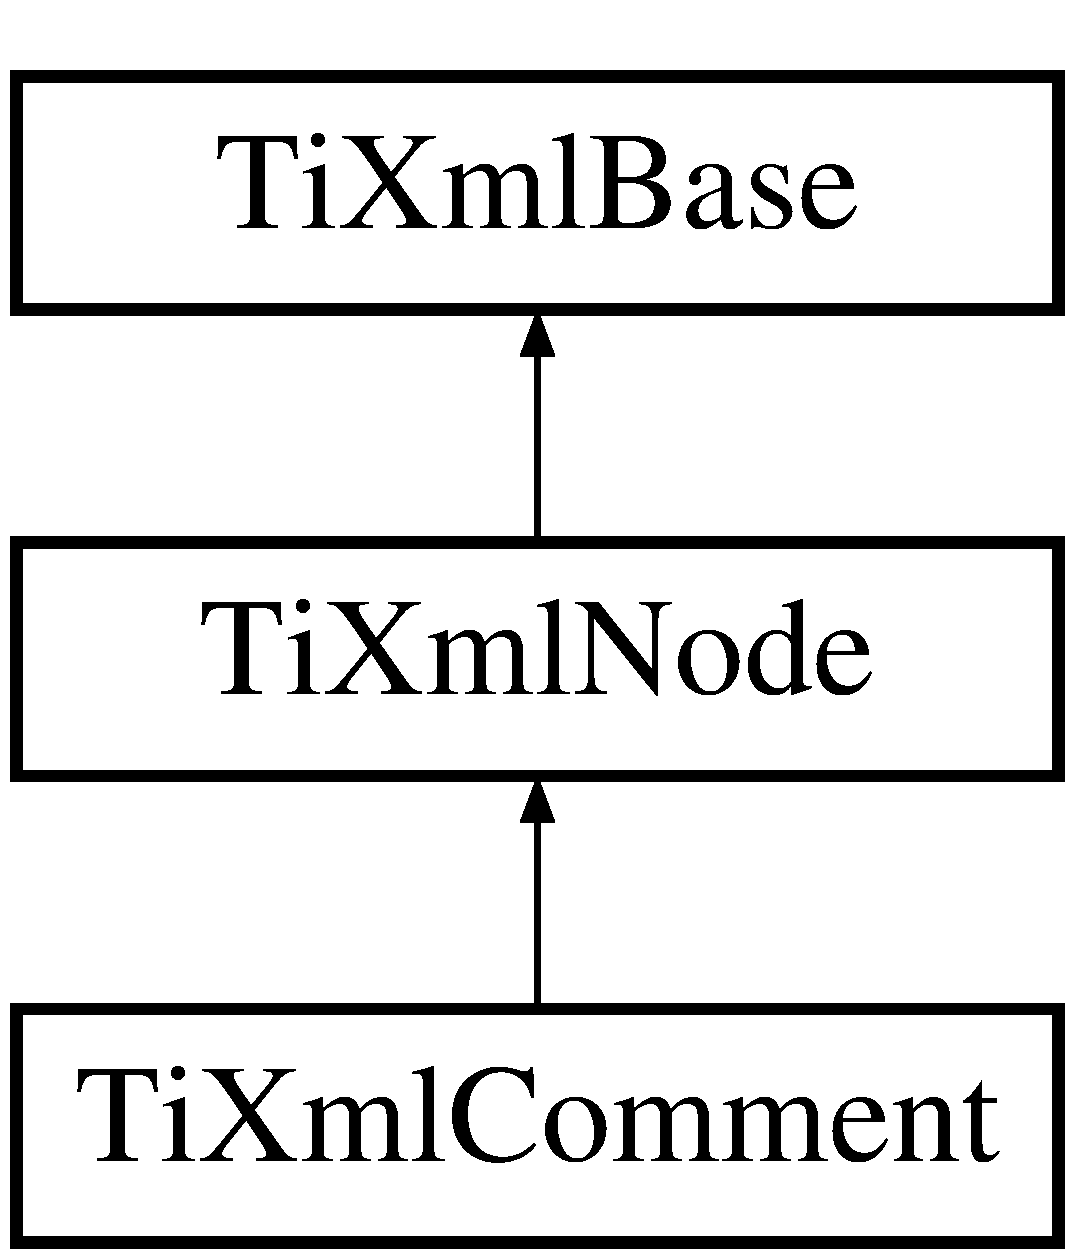
\includegraphics[height=3.000000cm]{class_ti_xml_comment}
\end{center}
\end{figure}
\subsection*{Public Member Functions}
\begin{DoxyCompactItemize}
\item 
\hypertarget{class_ti_xml_comment_aaa3252031d3e8bd3a2bf51a1c61201b7}{\hyperlink{class_ti_xml_comment_aaa3252031d3e8bd3a2bf51a1c61201b7}{Ti\+Xml\+Comment} ()}\label{class_ti_xml_comment_aaa3252031d3e8bd3a2bf51a1c61201b7}

\begin{DoxyCompactList}\small\item\em Constructs an empty comment. \end{DoxyCompactList}\item 
\hypertarget{class_ti_xml_comment_a37e7802ef17bc03ebe5ae79bf0713d47}{\hyperlink{class_ti_xml_comment_a37e7802ef17bc03ebe5ae79bf0713d47}{Ti\+Xml\+Comment} (const char $\ast$\+\_\+value)}\label{class_ti_xml_comment_a37e7802ef17bc03ebe5ae79bf0713d47}

\begin{DoxyCompactList}\small\item\em Construct a comment from text. \end{DoxyCompactList}\item 
\hypertarget{class_ti_xml_comment_afaec41ac2760ce946ba1590eb5708e50}{{\bfseries Ti\+Xml\+Comment} (const \hyperlink{class_ti_xml_comment}{Ti\+Xml\+Comment} \&)}\label{class_ti_xml_comment_afaec41ac2760ce946ba1590eb5708e50}

\item 
\hypertarget{class_ti_xml_comment_aeceedc15f8b8f9ca0b6136696339b3ac}{\hyperlink{class_ti_xml_comment}{Ti\+Xml\+Comment} \& {\bfseries operator=} (const \hyperlink{class_ti_xml_comment}{Ti\+Xml\+Comment} \&base)}\label{class_ti_xml_comment_aeceedc15f8b8f9ca0b6136696339b3ac}

\item 
\hypertarget{class_ti_xml_comment_a4f6590c9c9a2b63a48972655b78eb853}{virtual \hyperlink{class_ti_xml_node}{Ti\+Xml\+Node} $\ast$ \hyperlink{class_ti_xml_comment_a4f6590c9c9a2b63a48972655b78eb853}{Clone} () const }\label{class_ti_xml_comment_a4f6590c9c9a2b63a48972655b78eb853}

\begin{DoxyCompactList}\small\item\em Returns a copy of this Comment. \end{DoxyCompactList}\item 
virtual void \hyperlink{class_ti_xml_comment_a17398061d62c470f57801ce28fa33ad4}{Print} (F\+I\+L\+E $\ast$cfile, int depth) const 
\item 
\hypertarget{class_ti_xml_comment_a43bddc18ac057734b41d84653b71d3e0}{virtual const char $\ast$ {\bfseries Parse} (const char $\ast$p, \hyperlink{class_ti_xml_parsing_data}{Ti\+Xml\+Parsing\+Data} $\ast$data, Ti\+Xml\+Encoding encoding)}\label{class_ti_xml_comment_a43bddc18ac057734b41d84653b71d3e0}

\item 
\hypertarget{class_ti_xml_comment_a00fb4215c20a2399ea05ac9b9e7e68a0}{virtual const \hyperlink{class_ti_xml_comment}{Ti\+Xml\+Comment} $\ast$ \hyperlink{class_ti_xml_comment_a00fb4215c20a2399ea05ac9b9e7e68a0}{To\+Comment} () const }\label{class_ti_xml_comment_a00fb4215c20a2399ea05ac9b9e7e68a0}

\begin{DoxyCompactList}\small\item\em Cast to a more defined type. Will return null not of the requested type. \end{DoxyCompactList}\item 
\hypertarget{class_ti_xml_comment_acc7c7e07e13c23f17797d642981511df}{virtual \hyperlink{class_ti_xml_comment}{Ti\+Xml\+Comment} $\ast$ \hyperlink{class_ti_xml_comment_acc7c7e07e13c23f17797d642981511df}{To\+Comment} ()}\label{class_ti_xml_comment_acc7c7e07e13c23f17797d642981511df}

\begin{DoxyCompactList}\small\item\em Cast to a more defined type. Will return null not of the requested type. \end{DoxyCompactList}\item 
virtual bool \hyperlink{class_ti_xml_comment_a4382de0e50da973f11a23ea5852568bd}{Accept} (\hyperlink{class_ti_xml_visitor}{Ti\+Xml\+Visitor} $\ast$visitor) const 
\end{DoxyCompactItemize}
\subsection*{Protected Member Functions}
\begin{DoxyCompactItemize}
\item 
\hypertarget{class_ti_xml_comment_a3175b2f27628f4fb7a043897930cd934}{void {\bfseries Copy\+To} (\hyperlink{class_ti_xml_comment}{Ti\+Xml\+Comment} $\ast$target) const }\label{class_ti_xml_comment_a3175b2f27628f4fb7a043897930cd934}

\item 
\hypertarget{class_ti_xml_comment_a619467ff29c832b101e9b704a23c0357}{virtual void {\bfseries Stream\+In} (std\+::istream $\ast$in, T\+I\+X\+M\+L\+\_\+\+S\+T\+R\+I\+N\+G $\ast$tag)}\label{class_ti_xml_comment_a619467ff29c832b101e9b704a23c0357}

\end{DoxyCompactItemize}
\subsection*{Additional Inherited Members}


\subsection{Detailed Description}
An X\+M\+L comment. 

\subsection{Member Function Documentation}
\hypertarget{class_ti_xml_comment_a4382de0e50da973f11a23ea5852568bd}{\index{Ti\+Xml\+Comment@{Ti\+Xml\+Comment}!Accept@{Accept}}
\index{Accept@{Accept}!Ti\+Xml\+Comment@{Ti\+Xml\+Comment}}
\subsubsection[{Accept}]{\setlength{\rightskip}{0pt plus 5cm}bool Ti\+Xml\+Comment\+::\+Accept (
\begin{DoxyParamCaption}
\item[{{\bf Ti\+Xml\+Visitor} $\ast$}]{visitor}
\end{DoxyParamCaption}
) const\hspace{0.3cm}{\ttfamily [virtual]}}}\label{class_ti_xml_comment_a4382de0e50da973f11a23ea5852568bd}
Walk the X\+M\+L tree visiting this node and all of its children. 

Implements \hyperlink{class_ti_xml_node_acc0f88b7462c6cb73809d410a4f5bb86}{Ti\+Xml\+Node}.

\hypertarget{class_ti_xml_comment_a17398061d62c470f57801ce28fa33ad4}{\index{Ti\+Xml\+Comment@{Ti\+Xml\+Comment}!Print@{Print}}
\index{Print@{Print}!Ti\+Xml\+Comment@{Ti\+Xml\+Comment}}
\subsubsection[{Print}]{\setlength{\rightskip}{0pt plus 5cm}void Ti\+Xml\+Comment\+::\+Print (
\begin{DoxyParamCaption}
\item[{F\+I\+L\+E $\ast$}]{cfile, }
\item[{int}]{depth}
\end{DoxyParamCaption}
) const\hspace{0.3cm}{\ttfamily [virtual]}}}\label{class_ti_xml_comment_a17398061d62c470f57801ce28fa33ad4}
All Tiny\+Xml classes can print themselves to a filestream or the string class (\hyperlink{class_ti_xml_string}{Ti\+Xml\+String} in non-\/\+S\+T\+L mode, std\+::string in S\+T\+L mode.) Either or both cfile and str can be null.

This is a formatted print, and will insert tabs and newlines.

(For an unformatted stream, use the $<$$<$ operator.) 

Implements \hyperlink{class_ti_xml_base_a0de56b3f2ef14c65091a3b916437b512}{Ti\+Xml\+Base}.



The documentation for this class was generated from the following files\+:\begin{DoxyCompactItemize}
\item 
C\+:/\+Users/\+Avenger/\+Documents/\+Git\+Hub/\+Projet-\/\+Tamagoshi/includes/tinyxml/tinyxml.\+h\item 
C\+:/\+Users/\+Avenger/\+Documents/\+Git\+Hub/\+Projet-\/\+Tamagoshi/includes/tinyxml/tinyxml.\+cpp\item 
C\+:/\+Users/\+Avenger/\+Documents/\+Git\+Hub/\+Projet-\/\+Tamagoshi/includes/tinyxml/tinyxmlparser.\+cpp\end{DoxyCompactItemize}

\hypertarget{struct_ti_xml_cursor}{\section{Ti\+Xml\+Cursor Struct Reference}
\label{struct_ti_xml_cursor}\index{Ti\+Xml\+Cursor@{Ti\+Xml\+Cursor}}
}
\subsection*{Public Member Functions}
\begin{DoxyCompactItemize}
\item 
\hypertarget{struct_ti_xml_cursor_a1e6fa622b59dafb71b6efe595105dcdd}{void {\bfseries Clear} ()}\label{struct_ti_xml_cursor_a1e6fa622b59dafb71b6efe595105dcdd}

\end{DoxyCompactItemize}
\subsection*{Public Attributes}
\begin{DoxyCompactItemize}
\item 
\hypertarget{struct_ti_xml_cursor_a5b54dd949820c2db061e2be41f3effb3}{int {\bfseries row}}\label{struct_ti_xml_cursor_a5b54dd949820c2db061e2be41f3effb3}

\item 
\hypertarget{struct_ti_xml_cursor_a5694d7ed2c4d20109d350c14c417969d}{int {\bfseries col}}\label{struct_ti_xml_cursor_a5694d7ed2c4d20109d350c14c417969d}

\end{DoxyCompactItemize}


The documentation for this struct was generated from the following file\+:\begin{DoxyCompactItemize}
\item 
C\+:/\+Users/\+Avenger/\+Documents/\+Git\+Hub/\+Projet-\/\+Tamagoshi/includes/tinyxml/tinyxml.\+h\end{DoxyCompactItemize}

\hypertarget{class_ti_xml_declaration}{\section{Ti\+Xml\+Declaration Class Reference}
\label{class_ti_xml_declaration}\index{Ti\+Xml\+Declaration@{Ti\+Xml\+Declaration}}
}


{\ttfamily \#include $<$tinyxml.\+h$>$}

Inheritance diagram for Ti\+Xml\+Declaration\+:\begin{figure}[H]
\begin{center}
\leavevmode
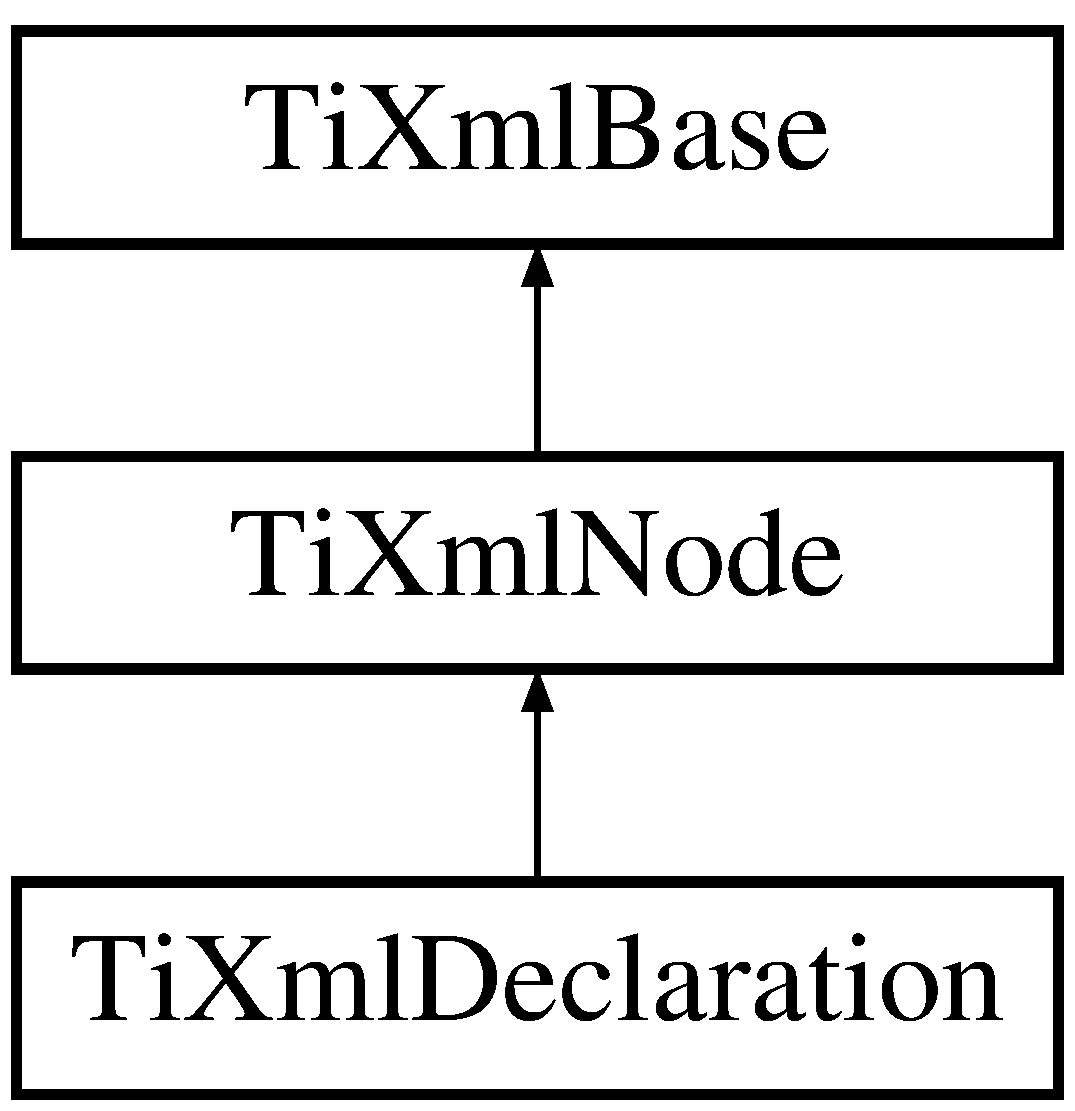
\includegraphics[height=3.000000cm]{class_ti_xml_declaration}
\end{center}
\end{figure}
\subsection*{Public Member Functions}
\begin{DoxyCompactItemize}
\item 
\hypertarget{class_ti_xml_declaration_aa0484d059bea0ea1acb47c9094382d79}{\hyperlink{class_ti_xml_declaration_aa0484d059bea0ea1acb47c9094382d79}{Ti\+Xml\+Declaration} ()}\label{class_ti_xml_declaration_aa0484d059bea0ea1acb47c9094382d79}

\begin{DoxyCompactList}\small\item\em Construct an empty declaration. \end{DoxyCompactList}\item 
\hypertarget{class_ti_xml_declaration_acd5556007c3c72209465081de39d9836}{\hyperlink{class_ti_xml_declaration_acd5556007c3c72209465081de39d9836}{Ti\+Xml\+Declaration} (const std\+::string \&\+\_\+version, const std\+::string \&\+\_\+encoding, const std\+::string \&\+\_\+standalone)}\label{class_ti_xml_declaration_acd5556007c3c72209465081de39d9836}

\begin{DoxyCompactList}\small\item\em Constructor. \end{DoxyCompactList}\item 
\hypertarget{class_ti_xml_declaration_a3b618d1c30c25e4b7a71f31a595ee298}{\hyperlink{class_ti_xml_declaration_a3b618d1c30c25e4b7a71f31a595ee298}{Ti\+Xml\+Declaration} (const char $\ast$\+\_\+version, const char $\ast$\+\_\+encoding, const char $\ast$\+\_\+standalone)}\label{class_ti_xml_declaration_a3b618d1c30c25e4b7a71f31a595ee298}

\begin{DoxyCompactList}\small\item\em Construct. \end{DoxyCompactList}\item 
\hypertarget{class_ti_xml_declaration_a58ac9042c342f7845c8491da0bb091e8}{{\bfseries Ti\+Xml\+Declaration} (const \hyperlink{class_ti_xml_declaration}{Ti\+Xml\+Declaration} \&copy)}\label{class_ti_xml_declaration_a58ac9042c342f7845c8491da0bb091e8}

\item 
\hypertarget{class_ti_xml_declaration_a3bc617efe11014ff2b1a9c5727c37a9a}{\hyperlink{class_ti_xml_declaration}{Ti\+Xml\+Declaration} \& {\bfseries operator=} (const \hyperlink{class_ti_xml_declaration}{Ti\+Xml\+Declaration} \&copy)}\label{class_ti_xml_declaration_a3bc617efe11014ff2b1a9c5727c37a9a}

\item 
\hypertarget{class_ti_xml_declaration_a02ee557b1a4545c3219ed377c103ec76}{const char $\ast$ \hyperlink{class_ti_xml_declaration_a02ee557b1a4545c3219ed377c103ec76}{Version} () const }\label{class_ti_xml_declaration_a02ee557b1a4545c3219ed377c103ec76}

\begin{DoxyCompactList}\small\item\em Version. Will return an empty string if none was found. \end{DoxyCompactList}\item 
\hypertarget{class_ti_xml_declaration_a5d974231f9e9a2f0542f15f3a46cdb76}{const char $\ast$ \hyperlink{class_ti_xml_declaration_a5d974231f9e9a2f0542f15f3a46cdb76}{Encoding} () const }\label{class_ti_xml_declaration_a5d974231f9e9a2f0542f15f3a46cdb76}

\begin{DoxyCompactList}\small\item\em Encoding. Will return an empty string if none was found. \end{DoxyCompactList}\item 
\hypertarget{class_ti_xml_declaration_a9ff06afc033d7ef730ec7c6825b97ad9}{const char $\ast$ \hyperlink{class_ti_xml_declaration_a9ff06afc033d7ef730ec7c6825b97ad9}{Standalone} () const }\label{class_ti_xml_declaration_a9ff06afc033d7ef730ec7c6825b97ad9}

\begin{DoxyCompactList}\small\item\em Is this a standalone document? \end{DoxyCompactList}\item 
\hypertarget{class_ti_xml_declaration_aff8231266d735943d8a7514a9c9822b9}{virtual \hyperlink{class_ti_xml_node}{Ti\+Xml\+Node} $\ast$ \hyperlink{class_ti_xml_declaration_aff8231266d735943d8a7514a9c9822b9}{Clone} () const }\label{class_ti_xml_declaration_aff8231266d735943d8a7514a9c9822b9}

\begin{DoxyCompactList}\small\item\em Creates a copy of this Declaration and returns it. \end{DoxyCompactList}\item 
\hypertarget{class_ti_xml_declaration_aa5ab32ec19d4eeecff4a9238c6c90565}{virtual void {\bfseries Print} (F\+I\+L\+E $\ast$cfile, int depth, T\+I\+X\+M\+L\+\_\+\+S\+T\+R\+I\+N\+G $\ast$str) const }\label{class_ti_xml_declaration_aa5ab32ec19d4eeecff4a9238c6c90565}

\item 
virtual void \hyperlink{class_ti_xml_declaration_abf6303db4bd05b5be554036817ff1cb4}{Print} (F\+I\+L\+E $\ast$cfile, int depth) const 
\item 
\hypertarget{class_ti_xml_declaration_a9839ea97ed687a2b7342fd7b0f04361b}{virtual const char $\ast$ {\bfseries Parse} (const char $\ast$p, \hyperlink{class_ti_xml_parsing_data}{Ti\+Xml\+Parsing\+Data} $\ast$data, Ti\+Xml\+Encoding encoding)}\label{class_ti_xml_declaration_a9839ea97ed687a2b7342fd7b0f04361b}

\item 
\hypertarget{class_ti_xml_declaration_a1e085d3fefd1dbf5ccdbff729931a967}{virtual const \hyperlink{class_ti_xml_declaration}{Ti\+Xml\+Declaration} $\ast$ \hyperlink{class_ti_xml_declaration_a1e085d3fefd1dbf5ccdbff729931a967}{To\+Declaration} () const }\label{class_ti_xml_declaration_a1e085d3fefd1dbf5ccdbff729931a967}

\begin{DoxyCompactList}\small\item\em Cast to a more defined type. Will return null not of the requested type. \end{DoxyCompactList}\item 
\hypertarget{class_ti_xml_declaration_a6bd3d1daddcaeb9543c24bfd090969ce}{virtual \hyperlink{class_ti_xml_declaration}{Ti\+Xml\+Declaration} $\ast$ \hyperlink{class_ti_xml_declaration_a6bd3d1daddcaeb9543c24bfd090969ce}{To\+Declaration} ()}\label{class_ti_xml_declaration_a6bd3d1daddcaeb9543c24bfd090969ce}

\begin{DoxyCompactList}\small\item\em Cast to a more defined type. Will return null not of the requested type. \end{DoxyCompactList}\item 
virtual bool \hyperlink{class_ti_xml_declaration_ab6a6b178161ba9abc2c35058de689864}{Accept} (\hyperlink{class_ti_xml_visitor}{Ti\+Xml\+Visitor} $\ast$visitor) const 
\end{DoxyCompactItemize}
\subsection*{Protected Member Functions}
\begin{DoxyCompactItemize}
\item 
\hypertarget{class_ti_xml_declaration_a9d08959f935421a593032bd3efb30c38}{void {\bfseries Copy\+To} (\hyperlink{class_ti_xml_declaration}{Ti\+Xml\+Declaration} $\ast$target) const }\label{class_ti_xml_declaration_a9d08959f935421a593032bd3efb30c38}

\item 
\hypertarget{class_ti_xml_declaration_af90df1c54c89b0f8dd56168419967610}{virtual void {\bfseries Stream\+In} (std\+::istream $\ast$in, T\+I\+X\+M\+L\+\_\+\+S\+T\+R\+I\+N\+G $\ast$tag)}\label{class_ti_xml_declaration_af90df1c54c89b0f8dd56168419967610}

\end{DoxyCompactItemize}
\subsection*{Additional Inherited Members}


\subsection{Detailed Description}
In correct X\+M\+L the declaration is the first entry in the file. \begin{DoxyVerb}    <?xml version="1.0" standalone="yes"?>
\end{DoxyVerb}


Tiny\+Xml will happily read or write files without a declaration, however. There are 3 possible attributes to the declaration\+: version, encoding, and standalone.

Note\+: In this version of the code, the attributes are handled as special cases, not generic attributes, simply because there can only be at most 3 and they are always the same. 

\subsection{Member Function Documentation}
\hypertarget{class_ti_xml_declaration_ab6a6b178161ba9abc2c35058de689864}{\index{Ti\+Xml\+Declaration@{Ti\+Xml\+Declaration}!Accept@{Accept}}
\index{Accept@{Accept}!Ti\+Xml\+Declaration@{Ti\+Xml\+Declaration}}
\subsubsection[{Accept}]{\setlength{\rightskip}{0pt plus 5cm}bool Ti\+Xml\+Declaration\+::\+Accept (
\begin{DoxyParamCaption}
\item[{{\bf Ti\+Xml\+Visitor} $\ast$}]{visitor}
\end{DoxyParamCaption}
) const\hspace{0.3cm}{\ttfamily [virtual]}}}\label{class_ti_xml_declaration_ab6a6b178161ba9abc2c35058de689864}
Walk the X\+M\+L tree visiting this node and all of its children. 

Implements \hyperlink{class_ti_xml_node_acc0f88b7462c6cb73809d410a4f5bb86}{Ti\+Xml\+Node}.

\hypertarget{class_ti_xml_declaration_abf6303db4bd05b5be554036817ff1cb4}{\index{Ti\+Xml\+Declaration@{Ti\+Xml\+Declaration}!Print@{Print}}
\index{Print@{Print}!Ti\+Xml\+Declaration@{Ti\+Xml\+Declaration}}
\subsubsection[{Print}]{\setlength{\rightskip}{0pt plus 5cm}virtual void Ti\+Xml\+Declaration\+::\+Print (
\begin{DoxyParamCaption}
\item[{F\+I\+L\+E $\ast$}]{cfile, }
\item[{int}]{depth}
\end{DoxyParamCaption}
) const\hspace{0.3cm}{\ttfamily [inline]}, {\ttfamily [virtual]}}}\label{class_ti_xml_declaration_abf6303db4bd05b5be554036817ff1cb4}
All Tiny\+Xml classes can print themselves to a filestream or the string class (\hyperlink{class_ti_xml_string}{Ti\+Xml\+String} in non-\/\+S\+T\+L mode, std\+::string in S\+T\+L mode.) Either or both cfile and str can be null.

This is a formatted print, and will insert tabs and newlines.

(For an unformatted stream, use the $<$$<$ operator.) 

Implements \hyperlink{class_ti_xml_base_a0de56b3f2ef14c65091a3b916437b512}{Ti\+Xml\+Base}.



The documentation for this class was generated from the following files\+:\begin{DoxyCompactItemize}
\item 
C\+:/\+Users/\+Avenger/\+Documents/\+Git\+Hub/\+Projet-\/\+Tamagoshi/includes/tinyxml/tinyxml.\+h\item 
C\+:/\+Users/\+Avenger/\+Documents/\+Git\+Hub/\+Projet-\/\+Tamagoshi/includes/tinyxml/tinyxml.\+cpp\item 
C\+:/\+Users/\+Avenger/\+Documents/\+Git\+Hub/\+Projet-\/\+Tamagoshi/includes/tinyxml/tinyxmlparser.\+cpp\end{DoxyCompactItemize}

\hypertarget{class_ti_xml_document}{\section{Ti\+Xml\+Document Class Reference}
\label{class_ti_xml_document}\index{Ti\+Xml\+Document@{Ti\+Xml\+Document}}
}


{\ttfamily \#include $<$tinyxml.\+h$>$}

Inheritance diagram for Ti\+Xml\+Document\+:\begin{figure}[H]
\begin{center}
\leavevmode
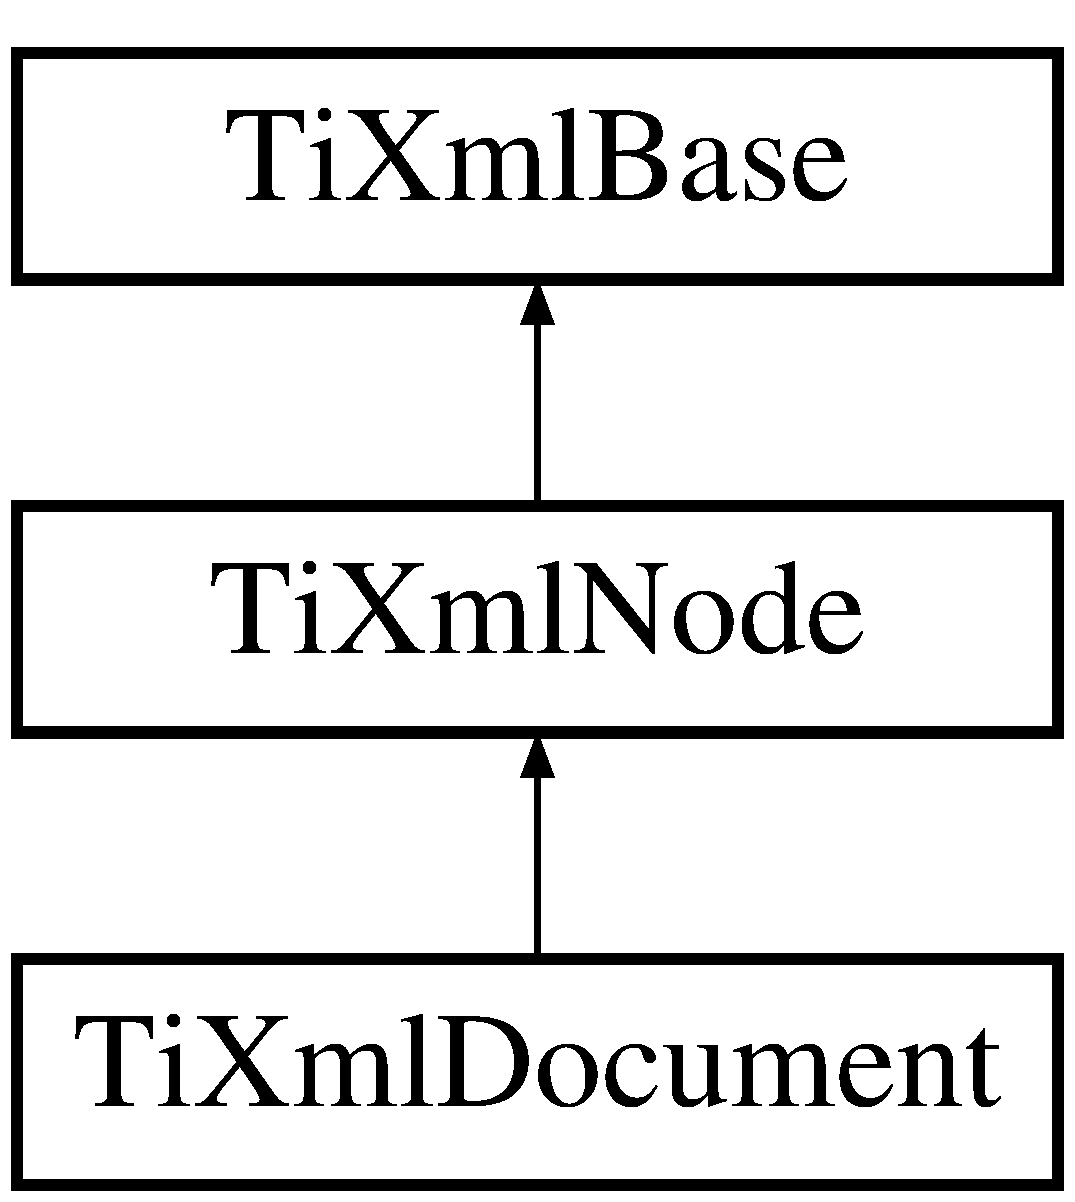
\includegraphics[height=3.000000cm]{class_ti_xml_document}
\end{center}
\end{figure}
\subsection*{Public Member Functions}
\begin{DoxyCompactItemize}
\item 
\hypertarget{class_ti_xml_document_a9f5e84335708fde98400230f9f12659c}{\hyperlink{class_ti_xml_document_a9f5e84335708fde98400230f9f12659c}{Ti\+Xml\+Document} ()}\label{class_ti_xml_document_a9f5e84335708fde98400230f9f12659c}

\begin{DoxyCompactList}\small\item\em Create an empty document, that has no name. \end{DoxyCompactList}\item 
\hypertarget{class_ti_xml_document_ae4508b452d0c3061db085f3db27b8396}{\hyperlink{class_ti_xml_document_ae4508b452d0c3061db085f3db27b8396}{Ti\+Xml\+Document} (const char $\ast$document\+Name)}\label{class_ti_xml_document_ae4508b452d0c3061db085f3db27b8396}

\begin{DoxyCompactList}\small\item\em Create a document with a name. The name of the document is also the filename of the xml. \end{DoxyCompactList}\item 
\hypertarget{class_ti_xml_document_a2c6e58fb99bfa76cc613f16840022225}{\hyperlink{class_ti_xml_document_a2c6e58fb99bfa76cc613f16840022225}{Ti\+Xml\+Document} (const std\+::string \&document\+Name)}\label{class_ti_xml_document_a2c6e58fb99bfa76cc613f16840022225}

\begin{DoxyCompactList}\small\item\em Constructor. \end{DoxyCompactList}\item 
\hypertarget{class_ti_xml_document_a323a7486e7da6099cdc19a5ff7e74b07}{{\bfseries Ti\+Xml\+Document} (const \hyperlink{class_ti_xml_document}{Ti\+Xml\+Document} \&copy)}\label{class_ti_xml_document_a323a7486e7da6099cdc19a5ff7e74b07}

\item 
\hypertarget{class_ti_xml_document_aa56fd4dbe8917d2033d865909e2d737e}{\hyperlink{class_ti_xml_document}{Ti\+Xml\+Document} \& {\bfseries operator=} (const \hyperlink{class_ti_xml_document}{Ti\+Xml\+Document} \&copy)}\label{class_ti_xml_document_aa56fd4dbe8917d2033d865909e2d737e}

\item 
bool \hyperlink{class_ti_xml_document_a4c852a889c02cf251117fd1d9fe1845f}{Load\+File} (Ti\+Xml\+Encoding encoding=T\+I\+X\+M\+L\+\_\+\+D\+E\+F\+A\+U\+L\+T\+\_\+\+E\+N\+C\+O\+D\+I\+N\+G)
\item 
\hypertarget{class_ti_xml_document_a21c0aeb0d0a720169ad4ac89523ebe93}{bool \hyperlink{class_ti_xml_document_a21c0aeb0d0a720169ad4ac89523ebe93}{Save\+File} () const }\label{class_ti_xml_document_a21c0aeb0d0a720169ad4ac89523ebe93}

\begin{DoxyCompactList}\small\item\em Save a file using the current document value. Returns true if successful. \end{DoxyCompactList}\item 
\hypertarget{class_ti_xml_document_a879cdf5e981b8b2d2ef82f2546dd28fb}{bool \hyperlink{class_ti_xml_document_a879cdf5e981b8b2d2ef82f2546dd28fb}{Load\+File} (const char $\ast$filename, Ti\+Xml\+Encoding encoding=T\+I\+X\+M\+L\+\_\+\+D\+E\+F\+A\+U\+L\+T\+\_\+\+E\+N\+C\+O\+D\+I\+N\+G)}\label{class_ti_xml_document_a879cdf5e981b8b2d2ef82f2546dd28fb}

\begin{DoxyCompactList}\small\item\em Load a file using the given filename. Returns true if successful. \end{DoxyCompactList}\item 
\hypertarget{class_ti_xml_document_ae869f5ebf7fc54c4a1d737fb4689fd44}{bool \hyperlink{class_ti_xml_document_ae869f5ebf7fc54c4a1d737fb4689fd44}{Save\+File} (const char $\ast$filename) const }\label{class_ti_xml_document_ae869f5ebf7fc54c4a1d737fb4689fd44}

\begin{DoxyCompactList}\small\item\em Save a file using the given filename. Returns true if successful. \end{DoxyCompactList}\item 
bool \hyperlink{class_ti_xml_document_a41f6fe7200864d1dca663d230caf8db6}{Load\+File} (F\+I\+L\+E $\ast$, Ti\+Xml\+Encoding encoding=T\+I\+X\+M\+L\+\_\+\+D\+E\+F\+A\+U\+L\+T\+\_\+\+E\+N\+C\+O\+D\+I\+N\+G)
\item 
\hypertarget{class_ti_xml_document_acf1672b4538c6d1d441f9f108aea2bf4}{bool \hyperlink{class_ti_xml_document_acf1672b4538c6d1d441f9f108aea2bf4}{Save\+File} (F\+I\+L\+E $\ast$) const }\label{class_ti_xml_document_acf1672b4538c6d1d441f9f108aea2bf4}

\begin{DoxyCompactList}\small\item\em Save a file using the given F\+I\+L\+E$\ast$. Returns true if successful. \end{DoxyCompactList}\item 
bool \hyperlink{class_ti_xml_document_a18ae6ed34fed7991ebc220862dfac884}{Load\+File} (const std\+::string \&filename, Ti\+Xml\+Encoding encoding=T\+I\+X\+M\+L\+\_\+\+D\+E\+F\+A\+U\+L\+T\+\_\+\+E\+N\+C\+O\+D\+I\+N\+G)
\item 
\hypertarget{class_ti_xml_document_a3d4fae0463f3f03679ba0b7cf6f2df52}{bool \hyperlink{class_ti_xml_document_a3d4fae0463f3f03679ba0b7cf6f2df52}{Save\+File} (const std\+::string \&filename) const }\label{class_ti_xml_document_a3d4fae0463f3f03679ba0b7cf6f2df52}

\begin{DoxyCompactList}\small\item\em $<$ S\+T\+L std\+::string version. \end{DoxyCompactList}\item 
virtual const char $\ast$ \hyperlink{class_ti_xml_document_a789ad2f06f93d52bdb5570b2f3670289}{Parse} (const char $\ast$p, \hyperlink{class_ti_xml_parsing_data}{Ti\+Xml\+Parsing\+Data} $\ast$data=0, Ti\+Xml\+Encoding encoding=T\+I\+X\+M\+L\+\_\+\+D\+E\+F\+A\+U\+L\+T\+\_\+\+E\+N\+C\+O\+D\+I\+N\+G)
\item 
const \hyperlink{class_ti_xml_element}{Ti\+Xml\+Element} $\ast$ \hyperlink{class_ti_xml_document_ad09d17927f908f40efb406af2fb873be}{Root\+Element} () const 
\item 
\hypertarget{class_ti_xml_document_a0b43e762a23f938b06651bc90b8a1013}{\hyperlink{class_ti_xml_element}{Ti\+Xml\+Element} $\ast$ {\bfseries Root\+Element} ()}\label{class_ti_xml_document_a0b43e762a23f938b06651bc90b8a1013}

\item 
bool \hyperlink{class_ti_xml_document_a6dfc01a6e5d58e56acd537dfd3bdeb29}{Error} () const 
\item 
\hypertarget{class_ti_xml_document_a9d0f689f6e09ea494ea547be8d79c25e}{const char $\ast$ \hyperlink{class_ti_xml_document_a9d0f689f6e09ea494ea547be8d79c25e}{Error\+Desc} () const }\label{class_ti_xml_document_a9d0f689f6e09ea494ea547be8d79c25e}

\begin{DoxyCompactList}\small\item\em Contains a textual (english) description of the error if one occurs. \end{DoxyCompactList}\item 
int \hyperlink{class_ti_xml_document_af96fc2f3f9ec6422782bfe916c9e778f}{Error\+Id} () const 
\item 
int \hyperlink{class_ti_xml_document_af30efc75e804aa2e92fb8be3a8cb676e}{Error\+Row} () const 
\item 
\hypertarget{class_ti_xml_document_aa90bc630ee5203c6109ca5fad3323649}{int \hyperlink{class_ti_xml_document_aa90bc630ee5203c6109ca5fad3323649}{Error\+Col} () const }\label{class_ti_xml_document_aa90bc630ee5203c6109ca5fad3323649}

\begin{DoxyCompactList}\small\item\em The column where the error occured. See \hyperlink{class_ti_xml_document_af30efc75e804aa2e92fb8be3a8cb676e}{Error\+Row()} \end{DoxyCompactList}\item 
void \hyperlink{class_ti_xml_document_a51dac56316f89b35bdb7d0d433ba988e}{Set\+Tab\+Size} (int \+\_\+tabsize)
\item 
\hypertarget{class_ti_xml_document_a612360241b85bad0826b2a9ae9cda561}{int {\bfseries Tab\+Size} () const }\label{class_ti_xml_document_a612360241b85bad0826b2a9ae9cda561}

\item 
void \hyperlink{class_ti_xml_document_ac66b8c28db86363315712a3574e87c35}{Clear\+Error} ()
\item 
void \hyperlink{class_ti_xml_document_af08389ec70ee9b2de7f800e206a18510}{Print} () const 
\item 
\hypertarget{class_ti_xml_document_a7b1aea204fee266b70b9c105c8bf2ada}{virtual void \hyperlink{class_ti_xml_document_a7b1aea204fee266b70b9c105c8bf2ada}{Print} (F\+I\+L\+E $\ast$cfile, int depth=0) const }\label{class_ti_xml_document_a7b1aea204fee266b70b9c105c8bf2ada}

\begin{DoxyCompactList}\small\item\em Print this Document to a F\+I\+L\+E stream. \end{DoxyCompactList}\item 
\hypertarget{class_ti_xml_document_a735c23e318597b920c94eae77fa206de}{void {\bfseries Set\+Error} (int err, const char $\ast$error\+Location, \hyperlink{class_ti_xml_parsing_data}{Ti\+Xml\+Parsing\+Data} $\ast$prev\+Data, Ti\+Xml\+Encoding encoding)}\label{class_ti_xml_document_a735c23e318597b920c94eae77fa206de}

\item 
\hypertarget{class_ti_xml_document_a1dc977bde3e4fe85a8eb9d88a35ef5a4}{virtual const \hyperlink{class_ti_xml_document}{Ti\+Xml\+Document} $\ast$ \hyperlink{class_ti_xml_document_a1dc977bde3e4fe85a8eb9d88a35ef5a4}{To\+Document} () const }\label{class_ti_xml_document_a1dc977bde3e4fe85a8eb9d88a35ef5a4}

\begin{DoxyCompactList}\small\item\em Cast to a more defined type. Will return null not of the requested type. \end{DoxyCompactList}\item 
\hypertarget{class_ti_xml_document_a1025d942a1f328fd742d545e37efdd42}{virtual \hyperlink{class_ti_xml_document}{Ti\+Xml\+Document} $\ast$ \hyperlink{class_ti_xml_document_a1025d942a1f328fd742d545e37efdd42}{To\+Document} ()}\label{class_ti_xml_document_a1025d942a1f328fd742d545e37efdd42}

\begin{DoxyCompactList}\small\item\em Cast to a more defined type. Will return null not of the requested type. \end{DoxyCompactList}\item 
virtual bool \hyperlink{class_ti_xml_document_a3daab2f472418ef66315750202f762ae}{Accept} (\hyperlink{class_ti_xml_visitor}{Ti\+Xml\+Visitor} $\ast$content) const 
\end{DoxyCompactItemize}
\subsection*{Protected Member Functions}
\begin{DoxyCompactItemize}
\item 
virtual \hyperlink{class_ti_xml_node}{Ti\+Xml\+Node} $\ast$ \hyperlink{class_ti_xml_document_ac9e8f09b23454d953b32d1b65cd1409e}{Clone} () const 
\item 
\hypertarget{class_ti_xml_document_aceaada9ac29206fb660e0449c92b1295}{virtual void {\bfseries Stream\+In} (std\+::istream $\ast$in, T\+I\+X\+M\+L\+\_\+\+S\+T\+R\+I\+N\+G $\ast$tag)}\label{class_ti_xml_document_aceaada9ac29206fb660e0449c92b1295}

\end{DoxyCompactItemize}
\subsection*{Additional Inherited Members}


\subsection{Detailed Description}
Always the top level node. A document binds together all the X\+M\+L pieces. It can be saved, loaded, and printed to the screen. The 'value' of a document node is the xml file name. 

\subsection{Member Function Documentation}
\hypertarget{class_ti_xml_document_a3daab2f472418ef66315750202f762ae}{\index{Ti\+Xml\+Document@{Ti\+Xml\+Document}!Accept@{Accept}}
\index{Accept@{Accept}!Ti\+Xml\+Document@{Ti\+Xml\+Document}}
\subsubsection[{Accept}]{\setlength{\rightskip}{0pt plus 5cm}bool Ti\+Xml\+Document\+::\+Accept (
\begin{DoxyParamCaption}
\item[{{\bf Ti\+Xml\+Visitor} $\ast$}]{content}
\end{DoxyParamCaption}
) const\hspace{0.3cm}{\ttfamily [virtual]}}}\label{class_ti_xml_document_a3daab2f472418ef66315750202f762ae}
Walk the X\+M\+L tree visiting this node and all of its children. 

Implements \hyperlink{class_ti_xml_node_acc0f88b7462c6cb73809d410a4f5bb86}{Ti\+Xml\+Node}.

\hypertarget{class_ti_xml_document_ac66b8c28db86363315712a3574e87c35}{\index{Ti\+Xml\+Document@{Ti\+Xml\+Document}!Clear\+Error@{Clear\+Error}}
\index{Clear\+Error@{Clear\+Error}!Ti\+Xml\+Document@{Ti\+Xml\+Document}}
\subsubsection[{Clear\+Error}]{\setlength{\rightskip}{0pt plus 5cm}void Ti\+Xml\+Document\+::\+Clear\+Error (
\begin{DoxyParamCaption}
{}
\end{DoxyParamCaption}
)\hspace{0.3cm}{\ttfamily [inline]}}}\label{class_ti_xml_document_ac66b8c28db86363315712a3574e87c35}
If you have handled the error, it can be reset with this call. The error state is automatically cleared if you Parse a new X\+M\+L block. \hypertarget{class_ti_xml_document_ac9e8f09b23454d953b32d1b65cd1409e}{\index{Ti\+Xml\+Document@{Ti\+Xml\+Document}!Clone@{Clone}}
\index{Clone@{Clone}!Ti\+Xml\+Document@{Ti\+Xml\+Document}}
\subsubsection[{Clone}]{\setlength{\rightskip}{0pt plus 5cm}{\bf Ti\+Xml\+Node} $\ast$ Ti\+Xml\+Document\+::\+Clone (
\begin{DoxyParamCaption}
{}
\end{DoxyParamCaption}
) const\hspace{0.3cm}{\ttfamily [protected]}, {\ttfamily [virtual]}}}\label{class_ti_xml_document_ac9e8f09b23454d953b32d1b65cd1409e}
Create an exact duplicate of this node and return it. The memory must be deleted by the caller. 

Implements \hyperlink{class_ti_xml_node_a4508cc3a2d7a98e96a54cc09c37a78a4}{Ti\+Xml\+Node}.

\hypertarget{class_ti_xml_document_a6dfc01a6e5d58e56acd537dfd3bdeb29}{\index{Ti\+Xml\+Document@{Ti\+Xml\+Document}!Error@{Error}}
\index{Error@{Error}!Ti\+Xml\+Document@{Ti\+Xml\+Document}}
\subsubsection[{Error}]{\setlength{\rightskip}{0pt plus 5cm}bool Ti\+Xml\+Document\+::\+Error (
\begin{DoxyParamCaption}
{}
\end{DoxyParamCaption}
) const\hspace{0.3cm}{\ttfamily [inline]}}}\label{class_ti_xml_document_a6dfc01a6e5d58e56acd537dfd3bdeb29}
If an error occurs, Error will be set to true. Also,
\begin{DoxyItemize}
\item The \hyperlink{class_ti_xml_document_af96fc2f3f9ec6422782bfe916c9e778f}{Error\+Id()} will contain the integer identifier of the error (not generally useful)
\item The \hyperlink{class_ti_xml_document_a9d0f689f6e09ea494ea547be8d79c25e}{Error\+Desc()} method will return the name of the error. (very useful)
\item The \hyperlink{class_ti_xml_document_af30efc75e804aa2e92fb8be3a8cb676e}{Error\+Row()} and \hyperlink{class_ti_xml_document_aa90bc630ee5203c6109ca5fad3323649}{Error\+Col()} will return the location of the error (if known) 
\end{DoxyItemize}\hypertarget{class_ti_xml_document_af96fc2f3f9ec6422782bfe916c9e778f}{\index{Ti\+Xml\+Document@{Ti\+Xml\+Document}!Error\+Id@{Error\+Id}}
\index{Error\+Id@{Error\+Id}!Ti\+Xml\+Document@{Ti\+Xml\+Document}}
\subsubsection[{Error\+Id}]{\setlength{\rightskip}{0pt plus 5cm}int Ti\+Xml\+Document\+::\+Error\+Id (
\begin{DoxyParamCaption}
{}
\end{DoxyParamCaption}
) const\hspace{0.3cm}{\ttfamily [inline]}}}\label{class_ti_xml_document_af96fc2f3f9ec6422782bfe916c9e778f}
Generally, you probably want the error string ( \hyperlink{class_ti_xml_document_a9d0f689f6e09ea494ea547be8d79c25e}{Error\+Desc()} ). But if you prefer the Error\+Id, this function will fetch it. \hypertarget{class_ti_xml_document_af30efc75e804aa2e92fb8be3a8cb676e}{\index{Ti\+Xml\+Document@{Ti\+Xml\+Document}!Error\+Row@{Error\+Row}}
\index{Error\+Row@{Error\+Row}!Ti\+Xml\+Document@{Ti\+Xml\+Document}}
\subsubsection[{Error\+Row}]{\setlength{\rightskip}{0pt plus 5cm}int Ti\+Xml\+Document\+::\+Error\+Row (
\begin{DoxyParamCaption}
{}
\end{DoxyParamCaption}
) const\hspace{0.3cm}{\ttfamily [inline]}}}\label{class_ti_xml_document_af30efc75e804aa2e92fb8be3a8cb676e}
Returns the location (if known) of the error. The first column is column 1, and the first row is row 1. A value of 0 means the row and column wasn't applicable (memory errors, for example, have no row/column) or the parser lost the error. (An error in the error reporting, in that case.)

\begin{DoxySeeAlso}{See also}
\hyperlink{class_ti_xml_document_a51dac56316f89b35bdb7d0d433ba988e}{Set\+Tab\+Size}, \hyperlink{class_ti_xml_base_a024bceb070188df92c2a8d8852dd0853}{Row}, \hyperlink{class_ti_xml_base_ab54bfb9b70fe6dd276e7b279cab7f003}{Column} 
\end{DoxySeeAlso}
\hypertarget{class_ti_xml_document_a4c852a889c02cf251117fd1d9fe1845f}{\index{Ti\+Xml\+Document@{Ti\+Xml\+Document}!Load\+File@{Load\+File}}
\index{Load\+File@{Load\+File}!Ti\+Xml\+Document@{Ti\+Xml\+Document}}
\subsubsection[{Load\+File}]{\setlength{\rightskip}{0pt plus 5cm}bool Ti\+Xml\+Document\+::\+Load\+File (
\begin{DoxyParamCaption}
\item[{Ti\+Xml\+Encoding}]{encoding = {\ttfamily TIXML\+\_\+DEFAULT\+\_\+ENCODING}}
\end{DoxyParamCaption}
)}}\label{class_ti_xml_document_a4c852a889c02cf251117fd1d9fe1845f}
Load a file using the current document value. Returns true if successful. Will delete any existing document data before loading. \hypertarget{class_ti_xml_document_a41f6fe7200864d1dca663d230caf8db6}{\index{Ti\+Xml\+Document@{Ti\+Xml\+Document}!Load\+File@{Load\+File}}
\index{Load\+File@{Load\+File}!Ti\+Xml\+Document@{Ti\+Xml\+Document}}
\subsubsection[{Load\+File}]{\setlength{\rightskip}{0pt plus 5cm}bool Ti\+Xml\+Document\+::\+Load\+File (
\begin{DoxyParamCaption}
\item[{F\+I\+L\+E $\ast$}]{file, }
\item[{Ti\+Xml\+Encoding}]{encoding = {\ttfamily TIXML\+\_\+DEFAULT\+\_\+ENCODING}}
\end{DoxyParamCaption}
)}}\label{class_ti_xml_document_a41f6fe7200864d1dca663d230caf8db6}
Load a file using the given F\+I\+L\+E$\ast$. Returns true if successful. Note that this method doesn't stream -\/ the entire object pointed at by the F\+I\+L\+E$\ast$ will be interpreted as an X\+M\+L file. Tiny\+X\+M\+L doesn't stream in X\+M\+L from the current file location. Streaming may be added in the future. \hypertarget{class_ti_xml_document_a18ae6ed34fed7991ebc220862dfac884}{\index{Ti\+Xml\+Document@{Ti\+Xml\+Document}!Load\+File@{Load\+File}}
\index{Load\+File@{Load\+File}!Ti\+Xml\+Document@{Ti\+Xml\+Document}}
\subsubsection[{Load\+File}]{\setlength{\rightskip}{0pt plus 5cm}bool Ti\+Xml\+Document\+::\+Load\+File (
\begin{DoxyParamCaption}
\item[{const std\+::string \&}]{filename, }
\item[{Ti\+Xml\+Encoding}]{encoding = {\ttfamily TIXML\+\_\+DEFAULT\+\_\+ENCODING}}
\end{DoxyParamCaption}
)\hspace{0.3cm}{\ttfamily [inline]}}}\label{class_ti_xml_document_a18ae6ed34fed7991ebc220862dfac884}

\begin{DoxyParams}{Parameters}
{\em encoding} & S\+T\+L std\+::string version. \\
\hline
\end{DoxyParams}
\hypertarget{class_ti_xml_document_a789ad2f06f93d52bdb5570b2f3670289}{\index{Ti\+Xml\+Document@{Ti\+Xml\+Document}!Parse@{Parse}}
\index{Parse@{Parse}!Ti\+Xml\+Document@{Ti\+Xml\+Document}}
\subsubsection[{Parse}]{\setlength{\rightskip}{0pt plus 5cm}const char $\ast$ Ti\+Xml\+Document\+::\+Parse (
\begin{DoxyParamCaption}
\item[{const char $\ast$}]{p, }
\item[{{\bf Ti\+Xml\+Parsing\+Data} $\ast$}]{data = {\ttfamily 0}, }
\item[{Ti\+Xml\+Encoding}]{encoding = {\ttfamily TIXML\+\_\+DEFAULT\+\_\+ENCODING}}
\end{DoxyParamCaption}
)\hspace{0.3cm}{\ttfamily [virtual]}}}\label{class_ti_xml_document_a789ad2f06f93d52bdb5570b2f3670289}
Parse the given null terminated block of xml data. Passing in an encoding to this method (either T\+I\+X\+M\+L\+\_\+\+E\+N\+C\+O\+D\+I\+N\+G\+\_\+\+L\+E\+G\+A\+C\+Y or T\+I\+X\+M\+L\+\_\+\+E\+N\+C\+O\+D\+I\+N\+G\+\_\+\+U\+T\+F8 will force Tiny\+Xml to use that encoding, regardless of what Tiny\+Xml might otherwise try to detect. 

Implements \hyperlink{class_ti_xml_base}{Ti\+Xml\+Base}.

\hypertarget{class_ti_xml_document_af08389ec70ee9b2de7f800e206a18510}{\index{Ti\+Xml\+Document@{Ti\+Xml\+Document}!Print@{Print}}
\index{Print@{Print}!Ti\+Xml\+Document@{Ti\+Xml\+Document}}
\subsubsection[{Print}]{\setlength{\rightskip}{0pt plus 5cm}void Ti\+Xml\+Document\+::\+Print (
\begin{DoxyParamCaption}
{}
\end{DoxyParamCaption}
) const\hspace{0.3cm}{\ttfamily [inline]}}}\label{class_ti_xml_document_af08389ec70ee9b2de7f800e206a18510}
Write the document to standard out using formatted printing (\char`\"{}pretty print\char`\"{}). \hypertarget{class_ti_xml_document_ad09d17927f908f40efb406af2fb873be}{\index{Ti\+Xml\+Document@{Ti\+Xml\+Document}!Root\+Element@{Root\+Element}}
\index{Root\+Element@{Root\+Element}!Ti\+Xml\+Document@{Ti\+Xml\+Document}}
\subsubsection[{Root\+Element}]{\setlength{\rightskip}{0pt plus 5cm}const {\bf Ti\+Xml\+Element}$\ast$ Ti\+Xml\+Document\+::\+Root\+Element (
\begin{DoxyParamCaption}
{}
\end{DoxyParamCaption}
) const\hspace{0.3cm}{\ttfamily [inline]}}}\label{class_ti_xml_document_ad09d17927f908f40efb406af2fb873be}
Get the root element -- the only top level element -- of the document. In well formed X\+M\+L, there should only be one. Tiny\+Xml is tolerant of multiple elements at the document level. \hypertarget{class_ti_xml_document_a51dac56316f89b35bdb7d0d433ba988e}{\index{Ti\+Xml\+Document@{Ti\+Xml\+Document}!Set\+Tab\+Size@{Set\+Tab\+Size}}
\index{Set\+Tab\+Size@{Set\+Tab\+Size}!Ti\+Xml\+Document@{Ti\+Xml\+Document}}
\subsubsection[{Set\+Tab\+Size}]{\setlength{\rightskip}{0pt plus 5cm}void Ti\+Xml\+Document\+::\+Set\+Tab\+Size (
\begin{DoxyParamCaption}
\item[{int}]{\+\_\+tabsize}
\end{DoxyParamCaption}
)\hspace{0.3cm}{\ttfamily [inline]}}}\label{class_ti_xml_document_a51dac56316f89b35bdb7d0d433ba988e}
\hyperlink{class_ti_xml_document_a51dac56316f89b35bdb7d0d433ba988e}{Set\+Tab\+Size()} allows the error reporting functions (\hyperlink{class_ti_xml_document_af30efc75e804aa2e92fb8be3a8cb676e}{Error\+Row()} and \hyperlink{class_ti_xml_document_aa90bc630ee5203c6109ca5fad3323649}{Error\+Col()}) to report the correct values for row and column. It does not change the output or input in any way.

By calling this method, with a tab size greater than 0, the row and column of each node and attribute is stored when the file is loaded. Very useful for tracking the D\+O\+M back in to the source file.

The tab size is required for calculating the location of nodes. If not set, the default of 4 is used. The tabsize is set per document. Setting the tabsize to 0 disables row/column tracking.

Note that row and column tracking is not supported when using operator$>$$>$.

The tab size needs to be enabled before the parse or load. Correct usage\+: \begin{DoxyVerb}TiXmlDocument doc;
doc.SetTabSize( 8 );
doc.Load( "myfile.xml" );
\end{DoxyVerb}


\begin{DoxySeeAlso}{See also}
\hyperlink{class_ti_xml_base_a024bceb070188df92c2a8d8852dd0853}{Row}, \hyperlink{class_ti_xml_base_ab54bfb9b70fe6dd276e7b279cab7f003}{Column} 
\end{DoxySeeAlso}


The documentation for this class was generated from the following files\+:\begin{DoxyCompactItemize}
\item 
C\+:/\+Users/\+Avenger/\+Documents/\+Git\+Hub/\+Projet-\/\+Tamagoshi/includes/tinyxml/tinyxml.\+h\item 
C\+:/\+Users/\+Avenger/\+Documents/\+Git\+Hub/\+Projet-\/\+Tamagoshi/includes/tinyxml/tinyxml.\+cpp\item 
C\+:/\+Users/\+Avenger/\+Documents/\+Git\+Hub/\+Projet-\/\+Tamagoshi/includes/tinyxml/tinyxmlparser.\+cpp\end{DoxyCompactItemize}

\hypertarget{class_ti_xml_element}{\section{Ti\+Xml\+Element Class Reference}
\label{class_ti_xml_element}\index{Ti\+Xml\+Element@{Ti\+Xml\+Element}}
}


{\ttfamily \#include $<$tinyxml.\+h$>$}

Inheritance diagram for Ti\+Xml\+Element\+:\begin{figure}[H]
\begin{center}
\leavevmode
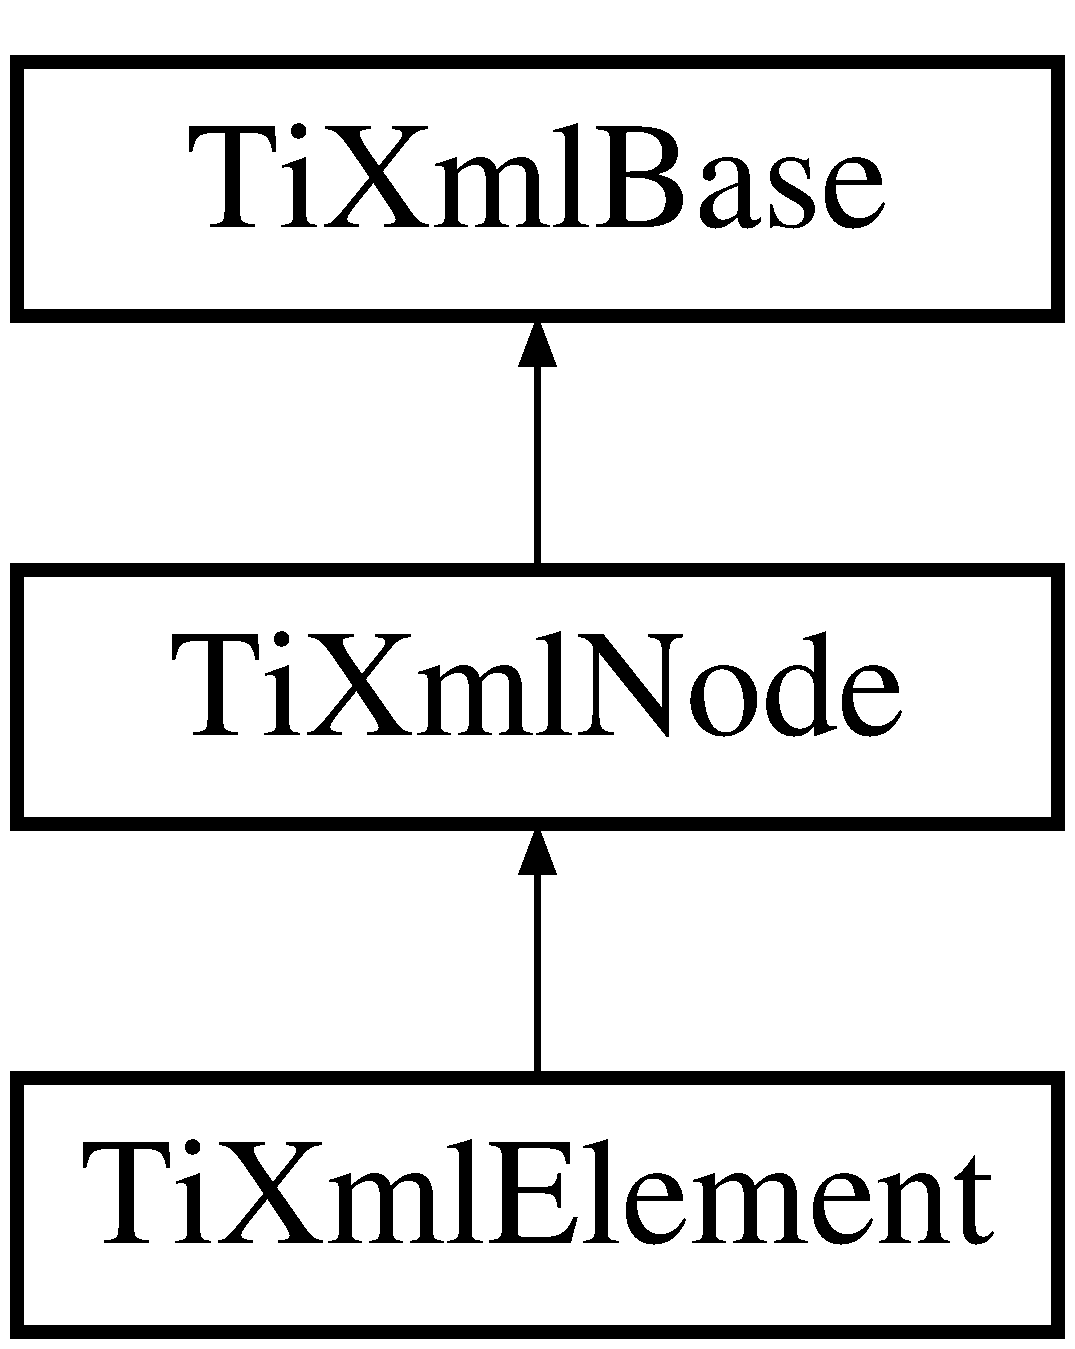
\includegraphics[height=3.000000cm]{class_ti_xml_element}
\end{center}
\end{figure}
\subsection*{Public Member Functions}
\begin{DoxyCompactItemize}
\item 
\hypertarget{class_ti_xml_element_a01bc3ab372d35da08efcbbe65ad90c60}{\hyperlink{class_ti_xml_element_a01bc3ab372d35da08efcbbe65ad90c60}{Ti\+Xml\+Element} (const char $\ast$in\+\_\+value)}\label{class_ti_xml_element_a01bc3ab372d35da08efcbbe65ad90c60}

\begin{DoxyCompactList}\small\item\em Construct an element. \end{DoxyCompactList}\item 
\hypertarget{class_ti_xml_element_a40fc2e3c1a955e2f78e1a32350d180e7}{\hyperlink{class_ti_xml_element_a40fc2e3c1a955e2f78e1a32350d180e7}{Ti\+Xml\+Element} (const std\+::string \&\+\_\+value)}\label{class_ti_xml_element_a40fc2e3c1a955e2f78e1a32350d180e7}

\begin{DoxyCompactList}\small\item\em std\+::string constructor. \end{DoxyCompactList}\item 
\hypertarget{class_ti_xml_element_a1ca4465f3c2eac6a60e641cd7f1d9f7e}{{\bfseries Ti\+Xml\+Element} (const \hyperlink{class_ti_xml_element}{Ti\+Xml\+Element} \&)}\label{class_ti_xml_element_a1ca4465f3c2eac6a60e641cd7f1d9f7e}

\item 
\hypertarget{class_ti_xml_element_ad58d300f4cfc0016ffa6861ebb718a0b}{\hyperlink{class_ti_xml_element}{Ti\+Xml\+Element} \& {\bfseries operator=} (const \hyperlink{class_ti_xml_element}{Ti\+Xml\+Element} \&base)}\label{class_ti_xml_element_ad58d300f4cfc0016ffa6861ebb718a0b}

\item 
const char $\ast$ \hyperlink{class_ti_xml_element_ac1e4691e9375ba4e665dce7e46a50a9c}{Attribute} (const char $\ast$name) const 
\item 
const char $\ast$ \hyperlink{class_ti_xml_element_aa9192e80567b5042dbded80b78c44339}{Attribute} (const char $\ast$name, int $\ast$i) const 
\item 
const char $\ast$ \hyperlink{class_ti_xml_element_aec4f727f8aa49b51248d80125d173136}{Attribute} (const char $\ast$name, double $\ast$d) const 
\item 
int \hyperlink{class_ti_xml_element_aea0bfe471380f281c5945770ddbf52b9}{Query\+Int\+Attribute} (const char $\ast$name, int $\ast$\+\_\+value) const 
\item 
\hypertarget{class_ti_xml_element_ae48df644f890ab86fa19839ac401f00d}{int \hyperlink{class_ti_xml_element_ae48df644f890ab86fa19839ac401f00d}{Query\+Unsigned\+Attribute} (const char $\ast$name, unsigned $\ast$\+\_\+value) const }\label{class_ti_xml_element_ae48df644f890ab86fa19839ac401f00d}

\begin{DoxyCompactList}\small\item\em Query\+Unsigned\+Attribute examines the attribute -\/ see \hyperlink{class_ti_xml_element_aea0bfe471380f281c5945770ddbf52b9}{Query\+Int\+Attribute()}. \end{DoxyCompactList}\item 
int \hyperlink{class_ti_xml_element_af4a1d3f88c28eb0f3115dc39ebd83fff}{Query\+Bool\+Attribute} (const char $\ast$name, bool $\ast$\+\_\+value) const 
\item 
\hypertarget{class_ti_xml_element_a898d7730ecc341f0bffc7a9dadbf1ce7}{int \hyperlink{class_ti_xml_element_a898d7730ecc341f0bffc7a9dadbf1ce7}{Query\+Double\+Attribute} (const char $\ast$name, double $\ast$\+\_\+value) const }\label{class_ti_xml_element_a898d7730ecc341f0bffc7a9dadbf1ce7}

\begin{DoxyCompactList}\small\item\em Query\+Double\+Attribute examines the attribute -\/ see \hyperlink{class_ti_xml_element_aea0bfe471380f281c5945770ddbf52b9}{Query\+Int\+Attribute()}. \end{DoxyCompactList}\item 
\hypertarget{class_ti_xml_element_aa04d3af11601ef5a5f88295203a843be}{int \hyperlink{class_ti_xml_element_aa04d3af11601ef5a5f88295203a843be}{Query\+Float\+Attribute} (const char $\ast$name, float $\ast$\+\_\+value) const }\label{class_ti_xml_element_aa04d3af11601ef5a5f88295203a843be}

\begin{DoxyCompactList}\small\item\em Query\+Float\+Attribute examines the attribute -\/ see \hyperlink{class_ti_xml_element_aea0bfe471380f281c5945770ddbf52b9}{Query\+Int\+Attribute()}. \end{DoxyCompactList}\item 
\hypertarget{class_ti_xml_element_a14321ac360efe906ed449d9db3fd9961}{int \hyperlink{class_ti_xml_element_a14321ac360efe906ed449d9db3fd9961}{Query\+String\+Attribute} (const char $\ast$name, std\+::string $\ast$\+\_\+value) const }\label{class_ti_xml_element_a14321ac360efe906ed449d9db3fd9961}

\begin{DoxyCompactList}\small\item\em Query\+String\+Attribute examines the attribute -\/ see \hyperlink{class_ti_xml_element_aea0bfe471380f281c5945770ddbf52b9}{Query\+Int\+Attribute()}. \end{DoxyCompactList}\item 
{\footnotesize template$<$typename T $>$ }\\int \hyperlink{class_ti_xml_element_a676f888438f8eb8d69a695ead195edb8}{Query\+Value\+Attribute} (const std\+::string \&name, T $\ast$out\+Value) const 
\item 
\hypertarget{class_ti_xml_element_a93fb47dab50d5f0d2912b789648c48ca}{int {\bfseries Query\+Value\+Attribute} (const std\+::string \&name, std\+::string $\ast$out\+Value) const }\label{class_ti_xml_element_a93fb47dab50d5f0d2912b789648c48ca}

\item 
void \hyperlink{class_ti_xml_element_abf0b3bd7f0e4c746a89ec6e7f101fc32}{Set\+Attribute} (const char $\ast$name, const char $\ast$\+\_\+value)
\item 
\hypertarget{class_ti_xml_element_a83b8b18d6ca253649ce378f8f5a2da49}{const std\+::string $\ast$ {\bfseries Attribute} (const std\+::string \&name) const }\label{class_ti_xml_element_a83b8b18d6ca253649ce378f8f5a2da49}

\item 
\hypertarget{class_ti_xml_element_aac36701ac5de73e9ef8c0b1d128e7782}{const std\+::string $\ast$ {\bfseries Attribute} (const std\+::string \&name, int $\ast$i) const }\label{class_ti_xml_element_aac36701ac5de73e9ef8c0b1d128e7782}

\item 
\hypertarget{class_ti_xml_element_a7131fe25a7e512f52ffa27518e108b7e}{const std\+::string $\ast$ {\bfseries Attribute} (const std\+::string \&name, double $\ast$d) const }\label{class_ti_xml_element_a7131fe25a7e512f52ffa27518e108b7e}

\item 
\hypertarget{class_ti_xml_element_ad79cb2416a5b94784f9a517add7e2d6d}{int {\bfseries Query\+Int\+Attribute} (const std\+::string \&name, int $\ast$\+\_\+value) const }\label{class_ti_xml_element_ad79cb2416a5b94784f9a517add7e2d6d}

\item 
\hypertarget{class_ti_xml_element_a157250e0c0303657d911f6991106ba73}{int {\bfseries Query\+Double\+Attribute} (const std\+::string \&name, double $\ast$\+\_\+value) const }\label{class_ti_xml_element_a157250e0c0303657d911f6991106ba73}

\item 
void \hyperlink{class_ti_xml_element_a80ed65b1d194c71c6c9986ae42337d7d}{Set\+Attribute} (const std\+::string \&name, const std\+::string \&\+\_\+value)
\begin{DoxyCompactList}\small\item\em S\+T\+L std\+::string form. \end{DoxyCompactList}\item 
\hypertarget{class_ti_xml_element_a6f18d54fbe25bbc527936ee65363b3c5}{void \hyperlink{class_ti_xml_element_a6f18d54fbe25bbc527936ee65363b3c5}{Set\+Attribute} (const std\+::string \&name, int \+\_\+value)}\label{class_ti_xml_element_a6f18d54fbe25bbc527936ee65363b3c5}

\begin{DoxyCompactList}\small\item\em S\+T\+L std\+::string form. \end{DoxyCompactList}\item 
\hypertarget{class_ti_xml_element_ac2112d423b39a93012b241f6baf4d3d3}{void {\bfseries Set\+Double\+Attribute} (const std\+::string \&name, double value)}\label{class_ti_xml_element_ac2112d423b39a93012b241f6baf4d3d3}

\item 
void \hyperlink{class_ti_xml_element_ace6f4be75e373726d4774073d666d1a7}{Set\+Attribute} (const char $\ast$name, int value)
\item 
void \hyperlink{class_ti_xml_element_a0d1dd975d75496778177e35abfe0ec0b}{Set\+Double\+Attribute} (const char $\ast$name, double value)
\item 
void \hyperlink{class_ti_xml_element_a56979767deca794376b1dfa69a525b2a}{Remove\+Attribute} (const char $\ast$name)
\item 
\hypertarget{class_ti_xml_element_a1afa6aea716511326a608e4c05df4f3a}{void \hyperlink{class_ti_xml_element_a1afa6aea716511326a608e4c05df4f3a}{Remove\+Attribute} (const std\+::string \&name)}\label{class_ti_xml_element_a1afa6aea716511326a608e4c05df4f3a}

\begin{DoxyCompactList}\small\item\em S\+T\+L std\+::string form. \end{DoxyCompactList}\item 
\hypertarget{class_ti_xml_element_a516054c9073647d6cb29b6abe9fa0592}{const \hyperlink{class_ti_xml_attribute}{Ti\+Xml\+Attribute} $\ast$ \hyperlink{class_ti_xml_element_a516054c9073647d6cb29b6abe9fa0592}{First\+Attribute} () const }\label{class_ti_xml_element_a516054c9073647d6cb29b6abe9fa0592}

\begin{DoxyCompactList}\small\item\em Access the first attribute in this element. \end{DoxyCompactList}\item 
\hypertarget{class_ti_xml_element_a4b33780fc565d38d6b54f640e0cf1737}{\hyperlink{class_ti_xml_attribute}{Ti\+Xml\+Attribute} $\ast$ {\bfseries First\+Attribute} ()}\label{class_ti_xml_element_a4b33780fc565d38d6b54f640e0cf1737}

\item 
\hypertarget{class_ti_xml_element_a86191b49f9177be132b85b14655f1381}{const \hyperlink{class_ti_xml_attribute}{Ti\+Xml\+Attribute} $\ast$ \hyperlink{class_ti_xml_element_a86191b49f9177be132b85b14655f1381}{Last\+Attribute} () const }\label{class_ti_xml_element_a86191b49f9177be132b85b14655f1381}

\begin{DoxyCompactList}\small\item\em Access the last attribute in this element. \end{DoxyCompactList}\item 
\hypertarget{class_ti_xml_element_a222f81cf06155cd108f2a68d4d176004}{\hyperlink{class_ti_xml_attribute}{Ti\+Xml\+Attribute} $\ast$ {\bfseries Last\+Attribute} ()}\label{class_ti_xml_element_a222f81cf06155cd108f2a68d4d176004}

\item 
const char $\ast$ \hyperlink{class_ti_xml_element_aa6dedd8a146acf3b1bc0903deb2d411a}{Get\+Text} () const 
\item 
\hypertarget{class_ti_xml_element_a13f6df105ebb1e8dc636e75cc883be32}{virtual \hyperlink{class_ti_xml_node}{Ti\+Xml\+Node} $\ast$ \hyperlink{class_ti_xml_element_a13f6df105ebb1e8dc636e75cc883be32}{Clone} () const }\label{class_ti_xml_element_a13f6df105ebb1e8dc636e75cc883be32}

\begin{DoxyCompactList}\small\item\em Creates a new Element and returns it -\/ the returned element is a copy. \end{DoxyCompactList}\item 
virtual void \hyperlink{class_ti_xml_element_ad9d0c008866982ab8d9aafae7e14d692}{Print} (F\+I\+L\+E $\ast$cfile, int depth) const 
\item 
\hypertarget{class_ti_xml_element_af95c9165159fd9dfdcc5b894a3fcf85b}{virtual const char $\ast$ {\bfseries Parse} (const char $\ast$p, \hyperlink{class_ti_xml_parsing_data}{Ti\+Xml\+Parsing\+Data} $\ast$data, Ti\+Xml\+Encoding encoding)}\label{class_ti_xml_element_af95c9165159fd9dfdcc5b894a3fcf85b}

\item 
\hypertarget{class_ti_xml_element_ac5b8d0e25fa23fd9acbb6d146082901c}{virtual const \hyperlink{class_ti_xml_element}{Ti\+Xml\+Element} $\ast$ \hyperlink{class_ti_xml_element_ac5b8d0e25fa23fd9acbb6d146082901c}{To\+Element} () const }\label{class_ti_xml_element_ac5b8d0e25fa23fd9acbb6d146082901c}

\begin{DoxyCompactList}\small\item\em Cast to a more defined type. Will return null not of the requested type. \end{DoxyCompactList}\item 
\hypertarget{class_ti_xml_element_a9def86337ea7a755eb41cac980f60c7a}{virtual \hyperlink{class_ti_xml_element}{Ti\+Xml\+Element} $\ast$ \hyperlink{class_ti_xml_element_a9def86337ea7a755eb41cac980f60c7a}{To\+Element} ()}\label{class_ti_xml_element_a9def86337ea7a755eb41cac980f60c7a}

\begin{DoxyCompactList}\small\item\em Cast to a more defined type. Will return null not of the requested type. \end{DoxyCompactList}\item 
virtual bool \hyperlink{class_ti_xml_element_a31ab28cc3b892a69254391d6bbe08df3}{Accept} (\hyperlink{class_ti_xml_visitor}{Ti\+Xml\+Visitor} $\ast$visitor) const 
\end{DoxyCompactItemize}
\subsection*{Protected Member Functions}
\begin{DoxyCompactItemize}
\item 
\hypertarget{class_ti_xml_element_a9e0c1983b840de4134f1f6bf7af00b0f}{void {\bfseries Copy\+To} (\hyperlink{class_ti_xml_element}{Ti\+Xml\+Element} $\ast$target) const }\label{class_ti_xml_element_a9e0c1983b840de4134f1f6bf7af00b0f}

\item 
\hypertarget{class_ti_xml_element_a5670933ec2d7d9763b9891acc05d7f7d}{void {\bfseries Clear\+This} ()}\label{class_ti_xml_element_a5670933ec2d7d9763b9891acc05d7f7d}

\item 
\hypertarget{class_ti_xml_element_a6884b491fb4708dae566f3ddc1476536}{virtual void {\bfseries Stream\+In} (std\+::istream $\ast$in, T\+I\+X\+M\+L\+\_\+\+S\+T\+R\+I\+N\+G $\ast$tag)}\label{class_ti_xml_element_a6884b491fb4708dae566f3ddc1476536}

\item 
\hypertarget{class_ti_xml_element_ac786bce103042d3837c4cc2ff6967d41}{const char $\ast$ {\bfseries Read\+Value} (const char $\ast$in, \hyperlink{class_ti_xml_parsing_data}{Ti\+Xml\+Parsing\+Data} $\ast$prev\+Data, Ti\+Xml\+Encoding encoding)}\label{class_ti_xml_element_ac786bce103042d3837c4cc2ff6967d41}

\end{DoxyCompactItemize}
\subsection*{Additional Inherited Members}


\subsection{Detailed Description}
The element is a container class. It has a value, the element name, and can contain other elements, text, comments, and unknowns. Elements also contain an arbitrary number of attributes. 

\subsection{Member Function Documentation}
\hypertarget{class_ti_xml_element_a31ab28cc3b892a69254391d6bbe08df3}{\index{Ti\+Xml\+Element@{Ti\+Xml\+Element}!Accept@{Accept}}
\index{Accept@{Accept}!Ti\+Xml\+Element@{Ti\+Xml\+Element}}
\subsubsection[{Accept}]{\setlength{\rightskip}{0pt plus 5cm}bool Ti\+Xml\+Element\+::\+Accept (
\begin{DoxyParamCaption}
\item[{{\bf Ti\+Xml\+Visitor} $\ast$}]{visitor}
\end{DoxyParamCaption}
) const\hspace{0.3cm}{\ttfamily [virtual]}}}\label{class_ti_xml_element_a31ab28cc3b892a69254391d6bbe08df3}
Walk the X\+M\+L tree visiting this node and all of its children. 

Implements \hyperlink{class_ti_xml_node_acc0f88b7462c6cb73809d410a4f5bb86}{Ti\+Xml\+Node}.

\hypertarget{class_ti_xml_element_ac1e4691e9375ba4e665dce7e46a50a9c}{\index{Ti\+Xml\+Element@{Ti\+Xml\+Element}!Attribute@{Attribute}}
\index{Attribute@{Attribute}!Ti\+Xml\+Element@{Ti\+Xml\+Element}}
\subsubsection[{Attribute}]{\setlength{\rightskip}{0pt plus 5cm}const char $\ast$ Ti\+Xml\+Element\+::\+Attribute (
\begin{DoxyParamCaption}
\item[{const char $\ast$}]{name}
\end{DoxyParamCaption}
) const}}\label{class_ti_xml_element_ac1e4691e9375ba4e665dce7e46a50a9c}
Given an attribute name, \hyperlink{class_ti_xml_element_ac1e4691e9375ba4e665dce7e46a50a9c}{Attribute()} returns the value for the attribute of that name, or null if none exists. \hypertarget{class_ti_xml_element_aa9192e80567b5042dbded80b78c44339}{\index{Ti\+Xml\+Element@{Ti\+Xml\+Element}!Attribute@{Attribute}}
\index{Attribute@{Attribute}!Ti\+Xml\+Element@{Ti\+Xml\+Element}}
\subsubsection[{Attribute}]{\setlength{\rightskip}{0pt plus 5cm}const char $\ast$ Ti\+Xml\+Element\+::\+Attribute (
\begin{DoxyParamCaption}
\item[{const char $\ast$}]{name, }
\item[{int $\ast$}]{i}
\end{DoxyParamCaption}
) const}}\label{class_ti_xml_element_aa9192e80567b5042dbded80b78c44339}
Given an attribute name, \hyperlink{class_ti_xml_element_ac1e4691e9375ba4e665dce7e46a50a9c}{Attribute()} returns the value for the attribute of that name, or null if none exists. If the attribute exists and can be converted to an integer, the integer value will be put in the return 'i', if 'i' is non-\/null. \hypertarget{class_ti_xml_element_aec4f727f8aa49b51248d80125d173136}{\index{Ti\+Xml\+Element@{Ti\+Xml\+Element}!Attribute@{Attribute}}
\index{Attribute@{Attribute}!Ti\+Xml\+Element@{Ti\+Xml\+Element}}
\subsubsection[{Attribute}]{\setlength{\rightskip}{0pt plus 5cm}const char $\ast$ Ti\+Xml\+Element\+::\+Attribute (
\begin{DoxyParamCaption}
\item[{const char $\ast$}]{name, }
\item[{double $\ast$}]{d}
\end{DoxyParamCaption}
) const}}\label{class_ti_xml_element_aec4f727f8aa49b51248d80125d173136}
Given an attribute name, \hyperlink{class_ti_xml_element_ac1e4691e9375ba4e665dce7e46a50a9c}{Attribute()} returns the value for the attribute of that name, or null if none exists. If the attribute exists and can be converted to an double, the double value will be put in the return 'd', if 'd' is non-\/null. \hypertarget{class_ti_xml_element_aa6dedd8a146acf3b1bc0903deb2d411a}{\index{Ti\+Xml\+Element@{Ti\+Xml\+Element}!Get\+Text@{Get\+Text}}
\index{Get\+Text@{Get\+Text}!Ti\+Xml\+Element@{Ti\+Xml\+Element}}
\subsubsection[{Get\+Text}]{\setlength{\rightskip}{0pt plus 5cm}const char $\ast$ Ti\+Xml\+Element\+::\+Get\+Text (
\begin{DoxyParamCaption}
{}
\end{DoxyParamCaption}
) const}}\label{class_ti_xml_element_aa6dedd8a146acf3b1bc0903deb2d411a}
Convenience function for easy access to the text inside an element. Although easy and concise, \hyperlink{class_ti_xml_element_aa6dedd8a146acf3b1bc0903deb2d411a}{Get\+Text()} is limited compared to getting the \hyperlink{class_ti_xml_text}{Ti\+Xml\+Text} child and accessing it directly.

If the first child of 'this' is a \hyperlink{class_ti_xml_text}{Ti\+Xml\+Text}, the \hyperlink{class_ti_xml_element_aa6dedd8a146acf3b1bc0903deb2d411a}{Get\+Text()} returns the character string of the Text node, else null is returned.

This is a convenient method for getting the text of simple contained text\+: \begin{DoxyVerb}<foo>This is text</foo>
const char* str = fooElement->GetText();
\end{DoxyVerb}


'str' will be a pointer to \char`\"{}\+This is text\char`\"{}.

Note that this function can be misleading. If the element foo was created from this X\+M\+L\+: \begin{DoxyVerb}<foo><b>This is text</b></foo>
\end{DoxyVerb}


then the value of str would be null. The first child node isn't a text node, it is another element. From this X\+M\+L\+: \begin{DoxyVerb}<foo>This is <b>text</b></foo>
\end{DoxyVerb}
 \hyperlink{class_ti_xml_element_aa6dedd8a146acf3b1bc0903deb2d411a}{Get\+Text()} will return \char`\"{}\+This is \char`\"{}.

W\+A\+R\+N\+I\+N\+G\+: \hyperlink{class_ti_xml_element_aa6dedd8a146acf3b1bc0903deb2d411a}{Get\+Text()} accesses a child node -\/ don't become confused with the similarly named \hyperlink{class_ti_xml_handle_a9fc739c8a18d160006f82572fc143d13}{Ti\+Xml\+Handle\+::\+Text()} and \hyperlink{class_ti_xml_node_a3ddfbcac78fbea041fad57e5c6d60a03}{Ti\+Xml\+Node\+::\+To\+Text()} which are safe type casts on the referenced node. \hypertarget{class_ti_xml_element_ad9d0c008866982ab8d9aafae7e14d692}{\index{Ti\+Xml\+Element@{Ti\+Xml\+Element}!Print@{Print}}
\index{Print@{Print}!Ti\+Xml\+Element@{Ti\+Xml\+Element}}
\subsubsection[{Print}]{\setlength{\rightskip}{0pt plus 5cm}void Ti\+Xml\+Element\+::\+Print (
\begin{DoxyParamCaption}
\item[{F\+I\+L\+E $\ast$}]{cfile, }
\item[{int}]{depth}
\end{DoxyParamCaption}
) const\hspace{0.3cm}{\ttfamily [virtual]}}}\label{class_ti_xml_element_ad9d0c008866982ab8d9aafae7e14d692}
All Tiny\+Xml classes can print themselves to a filestream or the string class (\hyperlink{class_ti_xml_string}{Ti\+Xml\+String} in non-\/\+S\+T\+L mode, std\+::string in S\+T\+L mode.) Either or both cfile and str can be null.

This is a formatted print, and will insert tabs and newlines.

(For an unformatted stream, use the $<$$<$ operator.) 

Implements \hyperlink{class_ti_xml_base_a0de56b3f2ef14c65091a3b916437b512}{Ti\+Xml\+Base}.

\hypertarget{class_ti_xml_element_af4a1d3f88c28eb0f3115dc39ebd83fff}{\index{Ti\+Xml\+Element@{Ti\+Xml\+Element}!Query\+Bool\+Attribute@{Query\+Bool\+Attribute}}
\index{Query\+Bool\+Attribute@{Query\+Bool\+Attribute}!Ti\+Xml\+Element@{Ti\+Xml\+Element}}
\subsubsection[{Query\+Bool\+Attribute}]{\setlength{\rightskip}{0pt plus 5cm}int Ti\+Xml\+Element\+::\+Query\+Bool\+Attribute (
\begin{DoxyParamCaption}
\item[{const char $\ast$}]{name, }
\item[{bool $\ast$}]{\+\_\+value}
\end{DoxyParamCaption}
) const}}\label{class_ti_xml_element_af4a1d3f88c28eb0f3115dc39ebd83fff}
Query\+Bool\+Attribute examines the attribute -\/ see \hyperlink{class_ti_xml_element_aea0bfe471380f281c5945770ddbf52b9}{Query\+Int\+Attribute()}. Note that '1', 'true', or 'yes' are considered true, while '0', 'false' and 'no' are considered false. \hypertarget{class_ti_xml_element_aea0bfe471380f281c5945770ddbf52b9}{\index{Ti\+Xml\+Element@{Ti\+Xml\+Element}!Query\+Int\+Attribute@{Query\+Int\+Attribute}}
\index{Query\+Int\+Attribute@{Query\+Int\+Attribute}!Ti\+Xml\+Element@{Ti\+Xml\+Element}}
\subsubsection[{Query\+Int\+Attribute}]{\setlength{\rightskip}{0pt plus 5cm}int Ti\+Xml\+Element\+::\+Query\+Int\+Attribute (
\begin{DoxyParamCaption}
\item[{const char $\ast$}]{name, }
\item[{int $\ast$}]{\+\_\+value}
\end{DoxyParamCaption}
) const}}\label{class_ti_xml_element_aea0bfe471380f281c5945770ddbf52b9}
Query\+Int\+Attribute examines the attribute -\/ it is an alternative to the \hyperlink{class_ti_xml_element_ac1e4691e9375ba4e665dce7e46a50a9c}{Attribute()} method with richer error checking. If the attribute is an integer, it is stored in 'value' and the call returns T\+I\+X\+M\+L\+\_\+\+S\+U\+C\+C\+E\+S\+S. If it is not an integer, it returns T\+I\+X\+M\+L\+\_\+\+W\+R\+O\+N\+G\+\_\+\+T\+Y\+P\+E. If the attribute does not exist, then T\+I\+X\+M\+L\+\_\+\+N\+O\+\_\+\+A\+T\+T\+R\+I\+B\+U\+T\+E is returned. \hypertarget{class_ti_xml_element_a676f888438f8eb8d69a695ead195edb8}{\index{Ti\+Xml\+Element@{Ti\+Xml\+Element}!Query\+Value\+Attribute@{Query\+Value\+Attribute}}
\index{Query\+Value\+Attribute@{Query\+Value\+Attribute}!Ti\+Xml\+Element@{Ti\+Xml\+Element}}
\subsubsection[{Query\+Value\+Attribute}]{\setlength{\rightskip}{0pt plus 5cm}template$<$typename T $>$ int Ti\+Xml\+Element\+::\+Query\+Value\+Attribute (
\begin{DoxyParamCaption}
\item[{const std\+::string \&}]{name, }
\item[{T $\ast$}]{out\+Value}
\end{DoxyParamCaption}
) const\hspace{0.3cm}{\ttfamily [inline]}}}\label{class_ti_xml_element_a676f888438f8eb8d69a695ead195edb8}
Template form of the attribute query which will try to read the attribute into the specified type. Very easy, very powerful, but be careful to make sure to call this with the correct type.

N\+O\+T\+E\+: This method doesn't work correctly for 'string' types that contain spaces.

\begin{DoxyReturn}{Returns}
T\+I\+X\+M\+L\+\_\+\+S\+U\+C\+C\+E\+S\+S, T\+I\+X\+M\+L\+\_\+\+W\+R\+O\+N\+G\+\_\+\+T\+Y\+P\+E, or T\+I\+X\+M\+L\+\_\+\+N\+O\+\_\+\+A\+T\+T\+R\+I\+B\+U\+T\+E 
\end{DoxyReturn}
\hypertarget{class_ti_xml_element_a56979767deca794376b1dfa69a525b2a}{\index{Ti\+Xml\+Element@{Ti\+Xml\+Element}!Remove\+Attribute@{Remove\+Attribute}}
\index{Remove\+Attribute@{Remove\+Attribute}!Ti\+Xml\+Element@{Ti\+Xml\+Element}}
\subsubsection[{Remove\+Attribute}]{\setlength{\rightskip}{0pt plus 5cm}void Ti\+Xml\+Element\+::\+Remove\+Attribute (
\begin{DoxyParamCaption}
\item[{const char $\ast$}]{name}
\end{DoxyParamCaption}
)}}\label{class_ti_xml_element_a56979767deca794376b1dfa69a525b2a}
Deletes an attribute with the given name. \hypertarget{class_ti_xml_element_abf0b3bd7f0e4c746a89ec6e7f101fc32}{\index{Ti\+Xml\+Element@{Ti\+Xml\+Element}!Set\+Attribute@{Set\+Attribute}}
\index{Set\+Attribute@{Set\+Attribute}!Ti\+Xml\+Element@{Ti\+Xml\+Element}}
\subsubsection[{Set\+Attribute}]{\setlength{\rightskip}{0pt plus 5cm}void Ti\+Xml\+Element\+::\+Set\+Attribute (
\begin{DoxyParamCaption}
\item[{const char $\ast$}]{name, }
\item[{const char $\ast$}]{\+\_\+value}
\end{DoxyParamCaption}
)}}\label{class_ti_xml_element_abf0b3bd7f0e4c746a89ec6e7f101fc32}
Sets an attribute of name to a given value. The attribute will be created if it does not exist, or changed if it does. \hypertarget{class_ti_xml_element_a80ed65b1d194c71c6c9986ae42337d7d}{\index{Ti\+Xml\+Element@{Ti\+Xml\+Element}!Set\+Attribute@{Set\+Attribute}}
\index{Set\+Attribute@{Set\+Attribute}!Ti\+Xml\+Element@{Ti\+Xml\+Element}}
\subsubsection[{Set\+Attribute}]{\setlength{\rightskip}{0pt plus 5cm}void Ti\+Xml\+Element\+::\+Set\+Attribute (
\begin{DoxyParamCaption}
\item[{const std\+::string \&}]{name, }
\item[{const std\+::string \&}]{\+\_\+value}
\end{DoxyParamCaption}
)}}\label{class_ti_xml_element_a80ed65b1d194c71c6c9986ae42337d7d}


S\+T\+L std\+::string form. 

S\+T\+L std\+::string form. \hypertarget{class_ti_xml_element_ace6f4be75e373726d4774073d666d1a7}{\index{Ti\+Xml\+Element@{Ti\+Xml\+Element}!Set\+Attribute@{Set\+Attribute}}
\index{Set\+Attribute@{Set\+Attribute}!Ti\+Xml\+Element@{Ti\+Xml\+Element}}
\subsubsection[{Set\+Attribute}]{\setlength{\rightskip}{0pt plus 5cm}void Ti\+Xml\+Element\+::\+Set\+Attribute (
\begin{DoxyParamCaption}
\item[{const char $\ast$}]{name, }
\item[{int}]{value}
\end{DoxyParamCaption}
)}}\label{class_ti_xml_element_ace6f4be75e373726d4774073d666d1a7}
Sets an attribute of name to a given value. The attribute will be created if it does not exist, or changed if it does. \hypertarget{class_ti_xml_element_a0d1dd975d75496778177e35abfe0ec0b}{\index{Ti\+Xml\+Element@{Ti\+Xml\+Element}!Set\+Double\+Attribute@{Set\+Double\+Attribute}}
\index{Set\+Double\+Attribute@{Set\+Double\+Attribute}!Ti\+Xml\+Element@{Ti\+Xml\+Element}}
\subsubsection[{Set\+Double\+Attribute}]{\setlength{\rightskip}{0pt plus 5cm}void Ti\+Xml\+Element\+::\+Set\+Double\+Attribute (
\begin{DoxyParamCaption}
\item[{const char $\ast$}]{name, }
\item[{double}]{value}
\end{DoxyParamCaption}
)}}\label{class_ti_xml_element_a0d1dd975d75496778177e35abfe0ec0b}
Sets an attribute of name to a given value. The attribute will be created if it does not exist, or changed if it does. 

The documentation for this class was generated from the following files\+:\begin{DoxyCompactItemize}
\item 
C\+:/\+Users/\+Avenger/\+Documents/\+Git\+Hub/\+Projet-\/\+Tamagoshi/includes/tinyxml/tinyxml.\+h\item 
C\+:/\+Users/\+Avenger/\+Documents/\+Git\+Hub/\+Projet-\/\+Tamagoshi/includes/tinyxml/tinyxml.\+cpp\item 
C\+:/\+Users/\+Avenger/\+Documents/\+Git\+Hub/\+Projet-\/\+Tamagoshi/includes/tinyxml/tinyxmlparser.\+cpp\end{DoxyCompactItemize}

\hypertarget{class_ti_xml_handle}{\section{Ti\+Xml\+Handle Class Reference}
\label{class_ti_xml_handle}\index{Ti\+Xml\+Handle@{Ti\+Xml\+Handle}}
}


{\ttfamily \#include $<$tinyxml.\+h$>$}

\subsection*{Public Member Functions}
\begin{DoxyCompactItemize}
\item 
\hypertarget{class_ti_xml_handle_aba18fd7bdefb942ecdea4bf4b8e29ec8}{\hyperlink{class_ti_xml_handle_aba18fd7bdefb942ecdea4bf4b8e29ec8}{Ti\+Xml\+Handle} (\hyperlink{class_ti_xml_node}{Ti\+Xml\+Node} $\ast$\+\_\+node)}\label{class_ti_xml_handle_aba18fd7bdefb942ecdea4bf4b8e29ec8}

\begin{DoxyCompactList}\small\item\em Create a handle from any node (at any depth of the tree.) This can be a null pointer. \end{DoxyCompactList}\item 
\hypertarget{class_ti_xml_handle_a236d7855e1e56ccc7b980630c48c7fd7}{\hyperlink{class_ti_xml_handle_a236d7855e1e56ccc7b980630c48c7fd7}{Ti\+Xml\+Handle} (const \hyperlink{class_ti_xml_handle}{Ti\+Xml\+Handle} \&ref)}\label{class_ti_xml_handle_a236d7855e1e56ccc7b980630c48c7fd7}

\begin{DoxyCompactList}\small\item\em Copy constructor. \end{DoxyCompactList}\item 
\hypertarget{class_ti_xml_handle_ad8e5dcf6a87882674203157f29f8e4db}{\hyperlink{class_ti_xml_handle}{Ti\+Xml\+Handle} {\bfseries operator=} (const \hyperlink{class_ti_xml_handle}{Ti\+Xml\+Handle} \&ref)}\label{class_ti_xml_handle_ad8e5dcf6a87882674203157f29f8e4db}

\item 
\hypertarget{class_ti_xml_handle_acdb1faaf88a700b40ca2c8d9aee21139}{\hyperlink{class_ti_xml_handle}{Ti\+Xml\+Handle} \hyperlink{class_ti_xml_handle_acdb1faaf88a700b40ca2c8d9aee21139}{First\+Child} () const }\label{class_ti_xml_handle_acdb1faaf88a700b40ca2c8d9aee21139}

\begin{DoxyCompactList}\small\item\em Return a handle to the first child node. \end{DoxyCompactList}\item 
\hypertarget{class_ti_xml_handle_a8c61f64ae9365d89c264f289085541f8}{\hyperlink{class_ti_xml_handle}{Ti\+Xml\+Handle} \hyperlink{class_ti_xml_handle_a8c61f64ae9365d89c264f289085541f8}{First\+Child} (const char $\ast$value) const }\label{class_ti_xml_handle_a8c61f64ae9365d89c264f289085541f8}

\begin{DoxyCompactList}\small\item\em Return a handle to the first child node with the given name. \end{DoxyCompactList}\item 
\hypertarget{class_ti_xml_handle_a24d1112e995e937e4dddb202d4113d4a}{\hyperlink{class_ti_xml_handle}{Ti\+Xml\+Handle} \hyperlink{class_ti_xml_handle_a24d1112e995e937e4dddb202d4113d4a}{First\+Child\+Element} () const }\label{class_ti_xml_handle_a24d1112e995e937e4dddb202d4113d4a}

\begin{DoxyCompactList}\small\item\em Return a handle to the first child element. \end{DoxyCompactList}\item 
\hypertarget{class_ti_xml_handle_af0aea751320f5e430fac6f8fff3b8dd4}{\hyperlink{class_ti_xml_handle}{Ti\+Xml\+Handle} \hyperlink{class_ti_xml_handle_af0aea751320f5e430fac6f8fff3b8dd4}{First\+Child\+Element} (const char $\ast$value) const }\label{class_ti_xml_handle_af0aea751320f5e430fac6f8fff3b8dd4}

\begin{DoxyCompactList}\small\item\em Return a handle to the first child element with the given name. \end{DoxyCompactList}\item 
\hyperlink{class_ti_xml_handle}{Ti\+Xml\+Handle} \hyperlink{class_ti_xml_handle_a072492b4be1acdb0db2d03cd8f71ccc4}{Child} (const char $\ast$value, int index) const 
\item 
\hyperlink{class_ti_xml_handle}{Ti\+Xml\+Handle} \hyperlink{class_ti_xml_handle_af9cf6a7d08a5da94a8924425ad0cd5ac}{Child} (int index) const 
\item 
\hyperlink{class_ti_xml_handle}{Ti\+Xml\+Handle} \hyperlink{class_ti_xml_handle_a979a3f850984a176ee884e394c7eed2d}{Child\+Element} (const char $\ast$value, int index) const 
\item 
\hyperlink{class_ti_xml_handle}{Ti\+Xml\+Handle} \hyperlink{class_ti_xml_handle_a8786475b9d1f1518492e3a46704c7ef0}{Child\+Element} (int index) const 
\item 
\hypertarget{class_ti_xml_handle_a8b10982dd39e74f3b068ca8952282d8a}{\hyperlink{class_ti_xml_handle}{Ti\+Xml\+Handle} {\bfseries First\+Child} (const std\+::string \&\+\_\+value) const }\label{class_ti_xml_handle_a8b10982dd39e74f3b068ca8952282d8a}

\item 
\hypertarget{class_ti_xml_handle_a743f1e9cc18b5658c158ed5c0c165354}{\hyperlink{class_ti_xml_handle}{Ti\+Xml\+Handle} {\bfseries First\+Child\+Element} (const std\+::string \&\+\_\+value) const }\label{class_ti_xml_handle_a743f1e9cc18b5658c158ed5c0c165354}

\item 
\hypertarget{class_ti_xml_handle_a5c4617db96789e9a5581dd5c12cdd287}{\hyperlink{class_ti_xml_handle}{Ti\+Xml\+Handle} {\bfseries Child} (const std\+::string \&\+\_\+value, int index) const }\label{class_ti_xml_handle_a5c4617db96789e9a5581dd5c12cdd287}

\item 
\hypertarget{class_ti_xml_handle_a2e5f7758156e6b29a8e7a423eca2cf5b}{\hyperlink{class_ti_xml_handle}{Ti\+Xml\+Handle} {\bfseries Child\+Element} (const std\+::string \&\+\_\+value, int index) const }\label{class_ti_xml_handle_a2e5f7758156e6b29a8e7a423eca2cf5b}

\item 
\hyperlink{class_ti_xml_node}{Ti\+Xml\+Node} $\ast$ \hyperlink{class_ti_xml_handle_af678e5088e83be67baf76f699756f2c3}{To\+Node} () const 
\item 
\hyperlink{class_ti_xml_element}{Ti\+Xml\+Element} $\ast$ \hyperlink{class_ti_xml_handle_abc6e7ed383a5fe1e52b0c0004b457b9e}{To\+Element} () const 
\item 
\hyperlink{class_ti_xml_text}{Ti\+Xml\+Text} $\ast$ \hyperlink{class_ti_xml_handle_a4ac53a652296203a5b5e13854d923586}{To\+Text} () const 
\item 
\hyperlink{class_ti_xml_unknown}{Ti\+Xml\+Unknown} $\ast$ \hyperlink{class_ti_xml_handle_a1381c17507a130767b1e23afc93b3674}{To\+Unknown} () const 
\item 
\hyperlink{class_ti_xml_node}{Ti\+Xml\+Node} $\ast$ \hyperlink{class_ti_xml_handle_ab44b723a8dc9af72838a303c079d0376}{Node} () const 
\item 
\hyperlink{class_ti_xml_element}{Ti\+Xml\+Element} $\ast$ \hyperlink{class_ti_xml_handle_acb5fe8388a526289ea65e817a51e05e7}{Element} () const 
\item 
\hyperlink{class_ti_xml_text}{Ti\+Xml\+Text} $\ast$ \hyperlink{class_ti_xml_handle_a9fc739c8a18d160006f82572fc143d13}{Text} () const 
\item 
\hyperlink{class_ti_xml_unknown}{Ti\+Xml\+Unknown} $\ast$ \hyperlink{class_ti_xml_handle_a49675b74357ba2aae124657a9a1ef465}{Unknown} () const 
\end{DoxyCompactItemize}


\subsection{Detailed Description}
A \hyperlink{class_ti_xml_handle}{Ti\+Xml\+Handle} is a class that wraps a node pointer with null checks; this is an incredibly useful thing. Note that \hyperlink{class_ti_xml_handle}{Ti\+Xml\+Handle} is not part of the Tiny\+Xml D\+O\+M structure. It is a separate utility class.

Take an example\+: \begin{DoxyVerb}<Document>
    <Element attributeA = "valueA">
        <Child attributeB = "value1" />
        <Child attributeB = "value2" />
    </Element>
<Document>
\end{DoxyVerb}


Assuming you want the value of \char`\"{}attribute\+B\char`\"{} in the 2nd \char`\"{}\+Child\char`\"{} element, it's very easy to write a {\itshape lot} of code that looks like\+:

\begin{DoxyVerb}TiXmlElement* root = document.FirstChildElement( "Document" );
if ( root )
{
    TiXmlElement* element = root->FirstChildElement( "Element" );
    if ( element )
    {
        TiXmlElement* child = element->FirstChildElement( "Child" );
        if ( child )
        {
            TiXmlElement* child2 = child->NextSiblingElement( "Child" );
            if ( child2 )
            {
                // Finally do something useful.
\end{DoxyVerb}


And that doesn't even cover \char`\"{}else\char`\"{} cases. \hyperlink{class_ti_xml_handle}{Ti\+Xml\+Handle} addresses the verbosity of such code. A \hyperlink{class_ti_xml_handle}{Ti\+Xml\+Handle} checks for null pointers so it is perfectly safe and correct to use\+:

\begin{DoxyVerb}TiXmlHandle docHandle( &document );
TiXmlElement* child2 = docHandle.FirstChild( "Document" ).FirstChild( "Element" ).Child( "Child", 1 ).ToElement();
if ( child2 )
{
    // do something useful
\end{DoxyVerb}


Which is M\+U\+C\+H more concise and useful.

It is also safe to copy handles -\/ internally they are nothing more than node pointers. \begin{DoxyVerb}TiXmlHandle handleCopy = handle;
\end{DoxyVerb}


What they should not be used for is iteration\+:

\begin{DoxyVerb}int i=0;
while ( true )
{
    TiXmlElement* child = docHandle.FirstChild( "Document" ).FirstChild( "Element" ).Child( "Child", i ).ToElement();
    if ( !child )
        break;
    // do something
    ++i;
}
\end{DoxyVerb}


It seems reasonable, but it is in fact two embedded while loops. The Child method is a linear walk to find the element, so this code would iterate much more than it needs to. Instead, prefer\+:

\begin{DoxyVerb}TiXmlElement* child = docHandle.FirstChild( "Document" ).FirstChild( "Element" ).FirstChild( "Child" ).ToElement();

for( child; child; child=child->NextSiblingElement() )
{
    // do something
}
\end{DoxyVerb}
 

\subsection{Member Function Documentation}
\hypertarget{class_ti_xml_handle_a072492b4be1acdb0db2d03cd8f71ccc4}{\index{Ti\+Xml\+Handle@{Ti\+Xml\+Handle}!Child@{Child}}
\index{Child@{Child}!Ti\+Xml\+Handle@{Ti\+Xml\+Handle}}
\subsubsection[{Child}]{\setlength{\rightskip}{0pt plus 5cm}{\bf Ti\+Xml\+Handle} Ti\+Xml\+Handle\+::\+Child (
\begin{DoxyParamCaption}
\item[{const char $\ast$}]{value, }
\item[{int}]{index}
\end{DoxyParamCaption}
) const}}\label{class_ti_xml_handle_a072492b4be1acdb0db2d03cd8f71ccc4}
Return a handle to the \char`\"{}index\char`\"{} child with the given name. The first child is 0, the second 1, etc. \hypertarget{class_ti_xml_handle_af9cf6a7d08a5da94a8924425ad0cd5ac}{\index{Ti\+Xml\+Handle@{Ti\+Xml\+Handle}!Child@{Child}}
\index{Child@{Child}!Ti\+Xml\+Handle@{Ti\+Xml\+Handle}}
\subsubsection[{Child}]{\setlength{\rightskip}{0pt plus 5cm}{\bf Ti\+Xml\+Handle} Ti\+Xml\+Handle\+::\+Child (
\begin{DoxyParamCaption}
\item[{int}]{index}
\end{DoxyParamCaption}
) const}}\label{class_ti_xml_handle_af9cf6a7d08a5da94a8924425ad0cd5ac}
Return a handle to the \char`\"{}index\char`\"{} child. The first child is 0, the second 1, etc. \hypertarget{class_ti_xml_handle_a979a3f850984a176ee884e394c7eed2d}{\index{Ti\+Xml\+Handle@{Ti\+Xml\+Handle}!Child\+Element@{Child\+Element}}
\index{Child\+Element@{Child\+Element}!Ti\+Xml\+Handle@{Ti\+Xml\+Handle}}
\subsubsection[{Child\+Element}]{\setlength{\rightskip}{0pt plus 5cm}{\bf Ti\+Xml\+Handle} Ti\+Xml\+Handle\+::\+Child\+Element (
\begin{DoxyParamCaption}
\item[{const char $\ast$}]{value, }
\item[{int}]{index}
\end{DoxyParamCaption}
) const}}\label{class_ti_xml_handle_a979a3f850984a176ee884e394c7eed2d}
Return a handle to the \char`\"{}index\char`\"{} child element with the given name. The first child element is 0, the second 1, etc. Note that only Ti\+Xml\+Elements are indexed\+: other types are not counted. \hypertarget{class_ti_xml_handle_a8786475b9d1f1518492e3a46704c7ef0}{\index{Ti\+Xml\+Handle@{Ti\+Xml\+Handle}!Child\+Element@{Child\+Element}}
\index{Child\+Element@{Child\+Element}!Ti\+Xml\+Handle@{Ti\+Xml\+Handle}}
\subsubsection[{Child\+Element}]{\setlength{\rightskip}{0pt plus 5cm}{\bf Ti\+Xml\+Handle} Ti\+Xml\+Handle\+::\+Child\+Element (
\begin{DoxyParamCaption}
\item[{int}]{index}
\end{DoxyParamCaption}
) const}}\label{class_ti_xml_handle_a8786475b9d1f1518492e3a46704c7ef0}
Return a handle to the \char`\"{}index\char`\"{} child element. The first child element is 0, the second 1, etc. Note that only Ti\+Xml\+Elements are indexed\+: other types are not counted. \hypertarget{class_ti_xml_handle_acb5fe8388a526289ea65e817a51e05e7}{\index{Ti\+Xml\+Handle@{Ti\+Xml\+Handle}!Element@{Element}}
\index{Element@{Element}!Ti\+Xml\+Handle@{Ti\+Xml\+Handle}}
\subsubsection[{Element}]{\setlength{\rightskip}{0pt plus 5cm}{\bf Ti\+Xml\+Element}$\ast$ Ti\+Xml\+Handle\+::\+Element (
\begin{DoxyParamCaption}
{}
\end{DoxyParamCaption}
) const\hspace{0.3cm}{\ttfamily [inline]}}}\label{class_ti_xml_handle_acb5fe8388a526289ea65e817a51e05e7}
\begin{DoxyRefDesc}{Deprecated}
\item[\hyperlink{deprecated__deprecated000002}{Deprecated}]use To\+Element. Return the handle as a \hyperlink{class_ti_xml_element}{Ti\+Xml\+Element}. This may return null. \end{DoxyRefDesc}
\hypertarget{class_ti_xml_handle_ab44b723a8dc9af72838a303c079d0376}{\index{Ti\+Xml\+Handle@{Ti\+Xml\+Handle}!Node@{Node}}
\index{Node@{Node}!Ti\+Xml\+Handle@{Ti\+Xml\+Handle}}
\subsubsection[{Node}]{\setlength{\rightskip}{0pt plus 5cm}{\bf Ti\+Xml\+Node}$\ast$ Ti\+Xml\+Handle\+::\+Node (
\begin{DoxyParamCaption}
{}
\end{DoxyParamCaption}
) const\hspace{0.3cm}{\ttfamily [inline]}}}\label{class_ti_xml_handle_ab44b723a8dc9af72838a303c079d0376}
\begin{DoxyRefDesc}{Deprecated}
\item[\hyperlink{deprecated__deprecated000001}{Deprecated}]use To\+Node. Return the handle as a \hyperlink{class_ti_xml_node}{Ti\+Xml\+Node}. This may return null. \end{DoxyRefDesc}
\hypertarget{class_ti_xml_handle_a9fc739c8a18d160006f82572fc143d13}{\index{Ti\+Xml\+Handle@{Ti\+Xml\+Handle}!Text@{Text}}
\index{Text@{Text}!Ti\+Xml\+Handle@{Ti\+Xml\+Handle}}
\subsubsection[{Text}]{\setlength{\rightskip}{0pt plus 5cm}{\bf Ti\+Xml\+Text}$\ast$ Ti\+Xml\+Handle\+::\+Text (
\begin{DoxyParamCaption}
{}
\end{DoxyParamCaption}
) const\hspace{0.3cm}{\ttfamily [inline]}}}\label{class_ti_xml_handle_a9fc739c8a18d160006f82572fc143d13}
\begin{DoxyRefDesc}{Deprecated}
\item[\hyperlink{deprecated__deprecated000003}{Deprecated}]use \hyperlink{class_ti_xml_handle_a4ac53a652296203a5b5e13854d923586}{To\+Text()} Return the handle as a \hyperlink{class_ti_xml_text}{Ti\+Xml\+Text}. This may return null. \end{DoxyRefDesc}
\hypertarget{class_ti_xml_handle_abc6e7ed383a5fe1e52b0c0004b457b9e}{\index{Ti\+Xml\+Handle@{Ti\+Xml\+Handle}!To\+Element@{To\+Element}}
\index{To\+Element@{To\+Element}!Ti\+Xml\+Handle@{Ti\+Xml\+Handle}}
\subsubsection[{To\+Element}]{\setlength{\rightskip}{0pt plus 5cm}{\bf Ti\+Xml\+Element}$\ast$ Ti\+Xml\+Handle\+::\+To\+Element (
\begin{DoxyParamCaption}
{}
\end{DoxyParamCaption}
) const\hspace{0.3cm}{\ttfamily [inline]}}}\label{class_ti_xml_handle_abc6e7ed383a5fe1e52b0c0004b457b9e}
Return the handle as a \hyperlink{class_ti_xml_element}{Ti\+Xml\+Element}. This may return null. \hypertarget{class_ti_xml_handle_af678e5088e83be67baf76f699756f2c3}{\index{Ti\+Xml\+Handle@{Ti\+Xml\+Handle}!To\+Node@{To\+Node}}
\index{To\+Node@{To\+Node}!Ti\+Xml\+Handle@{Ti\+Xml\+Handle}}
\subsubsection[{To\+Node}]{\setlength{\rightskip}{0pt plus 5cm}{\bf Ti\+Xml\+Node}$\ast$ Ti\+Xml\+Handle\+::\+To\+Node (
\begin{DoxyParamCaption}
{}
\end{DoxyParamCaption}
) const\hspace{0.3cm}{\ttfamily [inline]}}}\label{class_ti_xml_handle_af678e5088e83be67baf76f699756f2c3}
Return the handle as a \hyperlink{class_ti_xml_node}{Ti\+Xml\+Node}. This may return null. \hypertarget{class_ti_xml_handle_a4ac53a652296203a5b5e13854d923586}{\index{Ti\+Xml\+Handle@{Ti\+Xml\+Handle}!To\+Text@{To\+Text}}
\index{To\+Text@{To\+Text}!Ti\+Xml\+Handle@{Ti\+Xml\+Handle}}
\subsubsection[{To\+Text}]{\setlength{\rightskip}{0pt plus 5cm}{\bf Ti\+Xml\+Text}$\ast$ Ti\+Xml\+Handle\+::\+To\+Text (
\begin{DoxyParamCaption}
{}
\end{DoxyParamCaption}
) const\hspace{0.3cm}{\ttfamily [inline]}}}\label{class_ti_xml_handle_a4ac53a652296203a5b5e13854d923586}
Return the handle as a \hyperlink{class_ti_xml_text}{Ti\+Xml\+Text}. This may return null. \hypertarget{class_ti_xml_handle_a1381c17507a130767b1e23afc93b3674}{\index{Ti\+Xml\+Handle@{Ti\+Xml\+Handle}!To\+Unknown@{To\+Unknown}}
\index{To\+Unknown@{To\+Unknown}!Ti\+Xml\+Handle@{Ti\+Xml\+Handle}}
\subsubsection[{To\+Unknown}]{\setlength{\rightskip}{0pt plus 5cm}{\bf Ti\+Xml\+Unknown}$\ast$ Ti\+Xml\+Handle\+::\+To\+Unknown (
\begin{DoxyParamCaption}
{}
\end{DoxyParamCaption}
) const\hspace{0.3cm}{\ttfamily [inline]}}}\label{class_ti_xml_handle_a1381c17507a130767b1e23afc93b3674}
Return the handle as a \hyperlink{class_ti_xml_unknown}{Ti\+Xml\+Unknown}. This may return null. \hypertarget{class_ti_xml_handle_a49675b74357ba2aae124657a9a1ef465}{\index{Ti\+Xml\+Handle@{Ti\+Xml\+Handle}!Unknown@{Unknown}}
\index{Unknown@{Unknown}!Ti\+Xml\+Handle@{Ti\+Xml\+Handle}}
\subsubsection[{Unknown}]{\setlength{\rightskip}{0pt plus 5cm}{\bf Ti\+Xml\+Unknown}$\ast$ Ti\+Xml\+Handle\+::\+Unknown (
\begin{DoxyParamCaption}
{}
\end{DoxyParamCaption}
) const\hspace{0.3cm}{\ttfamily [inline]}}}\label{class_ti_xml_handle_a49675b74357ba2aae124657a9a1ef465}
\begin{DoxyRefDesc}{Deprecated}
\item[\hyperlink{deprecated__deprecated000004}{Deprecated}]use \hyperlink{class_ti_xml_handle_a1381c17507a130767b1e23afc93b3674}{To\+Unknown()} Return the handle as a \hyperlink{class_ti_xml_unknown}{Ti\+Xml\+Unknown}. This may return null. \end{DoxyRefDesc}


The documentation for this class was generated from the following files\+:\begin{DoxyCompactItemize}
\item 
C\+:/\+Users/\+Avenger/\+Documents/\+Git\+Hub/\+Projet-\/\+Tamagoshi/includes/tinyxml/tinyxml.\+h\item 
C\+:/\+Users/\+Avenger/\+Documents/\+Git\+Hub/\+Projet-\/\+Tamagoshi/includes/tinyxml/tinyxml.\+cpp\end{DoxyCompactItemize}

\hypertarget{class_ti_xml_node}{\section{Ti\+Xml\+Node Class Reference}
\label{class_ti_xml_node}\index{Ti\+Xml\+Node@{Ti\+Xml\+Node}}
}


{\ttfamily \#include $<$tinyxml.\+h$>$}

Inheritance diagram for Ti\+Xml\+Node\+:\begin{figure}[H]
\begin{center}
\leavevmode
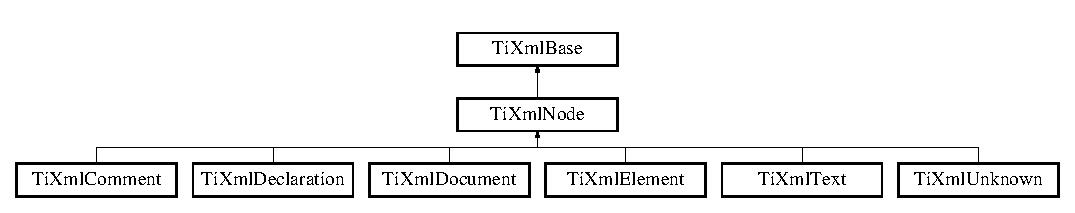
\includegraphics[height=2.413793cm]{class_ti_xml_node}
\end{center}
\end{figure}
\subsection*{Public Types}
\begin{DoxyCompactItemize}
\item 
enum \hyperlink{class_ti_xml_node_a836eded4920ab9e9ef28496f48cd95a2}{Node\+Type} \{ \\*
{\bfseries T\+I\+N\+Y\+X\+M\+L\+\_\+\+D\+O\+C\+U\+M\+E\+N\+T}, 
{\bfseries T\+I\+N\+Y\+X\+M\+L\+\_\+\+E\+L\+E\+M\+E\+N\+T}, 
{\bfseries T\+I\+N\+Y\+X\+M\+L\+\_\+\+C\+O\+M\+M\+E\+N\+T}, 
{\bfseries T\+I\+N\+Y\+X\+M\+L\+\_\+\+U\+N\+K\+N\+O\+W\+N}, 
\\*
{\bfseries T\+I\+N\+Y\+X\+M\+L\+\_\+\+T\+E\+X\+T}, 
{\bfseries T\+I\+N\+Y\+X\+M\+L\+\_\+\+D\+E\+C\+L\+A\+R\+A\+T\+I\+O\+N}, 
{\bfseries T\+I\+N\+Y\+X\+M\+L\+\_\+\+T\+Y\+P\+E\+C\+O\+U\+N\+T}
 \}
\end{DoxyCompactItemize}
\subsection*{Public Member Functions}
\begin{DoxyCompactItemize}
\item 
const char $\ast$ \hyperlink{class_ti_xml_node_a77943eb90d12c2892b1337a9f5918b41}{Value} () const 
\item 
const std\+::string \& \hyperlink{class_ti_xml_node_a6d9e505619d39bf50bfd9609c9169ea5}{Value\+Str} () const 
\item 
\hypertarget{class_ti_xml_node_a83ece13d2ea66dac66e0b21332229239}{const T\+I\+X\+M\+L\+\_\+\+S\+T\+R\+I\+N\+G \& {\bfseries Value\+T\+Str} () const }\label{class_ti_xml_node_a83ece13d2ea66dac66e0b21332229239}

\item 
void \hyperlink{class_ti_xml_node_a2a38329ca5d3f28f98ce932b8299ae90}{Set\+Value} (const char $\ast$\+\_\+value)
\item 
\hypertarget{class_ti_xml_node_a2598d5f448042c1abbeae4503dd45ff2}{void \hyperlink{class_ti_xml_node_a2598d5f448042c1abbeae4503dd45ff2}{Set\+Value} (const std\+::string \&\+\_\+value)}\label{class_ti_xml_node_a2598d5f448042c1abbeae4503dd45ff2}

\begin{DoxyCompactList}\small\item\em S\+T\+L std\+::string form. \end{DoxyCompactList}\item 
\hypertarget{class_ti_xml_node_a708e7f953df61d4d2d12f73171550a4b}{void \hyperlink{class_ti_xml_node_a708e7f953df61d4d2d12f73171550a4b}{Clear} ()}\label{class_ti_xml_node_a708e7f953df61d4d2d12f73171550a4b}

\begin{DoxyCompactList}\small\item\em Delete all the children of this node. Does not affect 'this'. \end{DoxyCompactList}\item 
\hypertarget{class_ti_xml_node_ab643043132ffd794f8602685d34a982e}{\hyperlink{class_ti_xml_node}{Ti\+Xml\+Node} $\ast$ \hyperlink{class_ti_xml_node_ab643043132ffd794f8602685d34a982e}{Parent} ()}\label{class_ti_xml_node_ab643043132ffd794f8602685d34a982e}

\begin{DoxyCompactList}\small\item\em One step up the D\+O\+M. \end{DoxyCompactList}\item 
\hypertarget{class_ti_xml_node_a78878709e53066f06eb4fcbcdd3a5260}{const \hyperlink{class_ti_xml_node}{Ti\+Xml\+Node} $\ast$ {\bfseries Parent} () const }\label{class_ti_xml_node_a78878709e53066f06eb4fcbcdd3a5260}

\item 
\hypertarget{class_ti_xml_node_a44c8eee26bbe2d1b2762038df9dde2f0}{const \hyperlink{class_ti_xml_node}{Ti\+Xml\+Node} $\ast$ \hyperlink{class_ti_xml_node_a44c8eee26bbe2d1b2762038df9dde2f0}{First\+Child} () const }\label{class_ti_xml_node_a44c8eee26bbe2d1b2762038df9dde2f0}

\begin{DoxyCompactList}\small\item\em The first child of this node. Will be null if there are no children. \end{DoxyCompactList}\item 
\hypertarget{class_ti_xml_node_a5e97d69b7c0ebd27fb7286be56559b77}{\hyperlink{class_ti_xml_node}{Ti\+Xml\+Node} $\ast$ {\bfseries First\+Child} ()}\label{class_ti_xml_node_a5e97d69b7c0ebd27fb7286be56559b77}

\item 
const \hyperlink{class_ti_xml_node}{Ti\+Xml\+Node} $\ast$ \hyperlink{class_ti_xml_node_ab5f722624113c8203227de4f56576d31}{First\+Child} (const char $\ast$value) const 
\item 
\hypertarget{class_ti_xml_node_abc8bf32be6419ec453a731868de19554}{\hyperlink{class_ti_xml_node}{Ti\+Xml\+Node} $\ast$ \hyperlink{class_ti_xml_node_abc8bf32be6419ec453a731868de19554}{First\+Child} (const char $\ast$\+\_\+value)}\label{class_ti_xml_node_abc8bf32be6419ec453a731868de19554}

\begin{DoxyCompactList}\small\item\em The first child of this node with the matching 'value'. Will be null if none found. \end{DoxyCompactList}\item 
\hypertarget{class_ti_xml_node_a6d671107e00cca1d28cb2d7f3a87a21e}{const \hyperlink{class_ti_xml_node}{Ti\+Xml\+Node} $\ast$ {\bfseries Last\+Child} () const }\label{class_ti_xml_node_a6d671107e00cca1d28cb2d7f3a87a21e}

\item 
\hypertarget{class_ti_xml_node_a6432d2b2495f6caf9cb4278df706a031}{\hyperlink{class_ti_xml_node}{Ti\+Xml\+Node} $\ast$ \hyperlink{class_ti_xml_node_a6432d2b2495f6caf9cb4278df706a031}{Last\+Child} ()}\label{class_ti_xml_node_a6432d2b2495f6caf9cb4278df706a031}

\begin{DoxyCompactList}\small\item\em The last child of this node. Will be null if there are no children. \end{DoxyCompactList}\item 
\hypertarget{class_ti_xml_node_acdd3fdc436aa7433023310a041e5e63f}{const \hyperlink{class_ti_xml_node}{Ti\+Xml\+Node} $\ast$ {\bfseries Last\+Child} (const char $\ast$value) const }\label{class_ti_xml_node_acdd3fdc436aa7433023310a041e5e63f}

\item 
\hypertarget{class_ti_xml_node_abad5bf1059c48127b958711ef89e8e5d}{\hyperlink{class_ti_xml_node}{Ti\+Xml\+Node} $\ast$ \hyperlink{class_ti_xml_node_abad5bf1059c48127b958711ef89e8e5d}{Last\+Child} (const char $\ast$\+\_\+value)}\label{class_ti_xml_node_abad5bf1059c48127b958711ef89e8e5d}

\begin{DoxyCompactList}\small\item\em The last child of this node matching 'value'. Will be null if there are no children. \end{DoxyCompactList}\item 
\hypertarget{class_ti_xml_node_a07f6200a5956c723c5b52d70f29c46f6}{const \hyperlink{class_ti_xml_node}{Ti\+Xml\+Node} $\ast$ \hyperlink{class_ti_xml_node_a07f6200a5956c723c5b52d70f29c46f6}{First\+Child} (const std\+::string \&\+\_\+value) const }\label{class_ti_xml_node_a07f6200a5956c723c5b52d70f29c46f6}

\begin{DoxyCompactList}\small\item\em S\+T\+L std\+::string form. \end{DoxyCompactList}\item 
\hypertarget{class_ti_xml_node_a10d2669ccb5e29e02fcb0e4408685ef6}{\hyperlink{class_ti_xml_node}{Ti\+Xml\+Node} $\ast$ \hyperlink{class_ti_xml_node_a10d2669ccb5e29e02fcb0e4408685ef6}{First\+Child} (const std\+::string \&\+\_\+value)}\label{class_ti_xml_node_a10d2669ccb5e29e02fcb0e4408685ef6}

\begin{DoxyCompactList}\small\item\em S\+T\+L std\+::string form. \end{DoxyCompactList}\item 
\hypertarget{class_ti_xml_node_a256d0cdbfcfeccae83f3a1c9747a8b63}{const \hyperlink{class_ti_xml_node}{Ti\+Xml\+Node} $\ast$ \hyperlink{class_ti_xml_node_a256d0cdbfcfeccae83f3a1c9747a8b63}{Last\+Child} (const std\+::string \&\+\_\+value) const }\label{class_ti_xml_node_a256d0cdbfcfeccae83f3a1c9747a8b63}

\begin{DoxyCompactList}\small\item\em S\+T\+L std\+::string form. \end{DoxyCompactList}\item 
\hypertarget{class_ti_xml_node_a69772c9202f70553f940b15c06b07be3}{\hyperlink{class_ti_xml_node}{Ti\+Xml\+Node} $\ast$ \hyperlink{class_ti_xml_node_a69772c9202f70553f940b15c06b07be3}{Last\+Child} (const std\+::string \&\+\_\+value)}\label{class_ti_xml_node_a69772c9202f70553f940b15c06b07be3}

\begin{DoxyCompactList}\small\item\em S\+T\+L std\+::string form. \end{DoxyCompactList}\item 
const \hyperlink{class_ti_xml_node}{Ti\+Xml\+Node} $\ast$ \hyperlink{class_ti_xml_node_aaef7ac3978c4bb1cc8a24ffae7bced75}{Iterate\+Children} (const \hyperlink{class_ti_xml_node}{Ti\+Xml\+Node} $\ast$previous) const 
\item 
\hypertarget{class_ti_xml_node_a2358e747118fdbf0e467b1e4f7d03de1}{\hyperlink{class_ti_xml_node}{Ti\+Xml\+Node} $\ast$ {\bfseries Iterate\+Children} (const \hyperlink{class_ti_xml_node}{Ti\+Xml\+Node} $\ast$previous)}\label{class_ti_xml_node_a2358e747118fdbf0e467b1e4f7d03de1}

\item 
\hypertarget{class_ti_xml_node_af2b86dbe25d3d26fa48180edc5e2a9fc}{const \hyperlink{class_ti_xml_node}{Ti\+Xml\+Node} $\ast$ \hyperlink{class_ti_xml_node_af2b86dbe25d3d26fa48180edc5e2a9fc}{Iterate\+Children} (const char $\ast$value, const \hyperlink{class_ti_xml_node}{Ti\+Xml\+Node} $\ast$previous) const }\label{class_ti_xml_node_af2b86dbe25d3d26fa48180edc5e2a9fc}

\begin{DoxyCompactList}\small\item\em This flavor of Iterate\+Children searches for children with a particular 'value'. \end{DoxyCompactList}\item 
\hypertarget{class_ti_xml_node_a67ba8275e533e6f76340236c42ea0aea}{\hyperlink{class_ti_xml_node}{Ti\+Xml\+Node} $\ast$ {\bfseries Iterate\+Children} (const char $\ast$\+\_\+value, const \hyperlink{class_ti_xml_node}{Ti\+Xml\+Node} $\ast$previous)}\label{class_ti_xml_node_a67ba8275e533e6f76340236c42ea0aea}

\item 
\hypertarget{class_ti_xml_node_a1cbaaf8e82c09ad763d52616d75724df}{const \hyperlink{class_ti_xml_node}{Ti\+Xml\+Node} $\ast$ \hyperlink{class_ti_xml_node_a1cbaaf8e82c09ad763d52616d75724df}{Iterate\+Children} (const std\+::string \&\+\_\+value, const \hyperlink{class_ti_xml_node}{Ti\+Xml\+Node} $\ast$previous) const }\label{class_ti_xml_node_a1cbaaf8e82c09ad763d52616d75724df}

\begin{DoxyCompactList}\small\item\em S\+T\+L std\+::string form. \end{DoxyCompactList}\item 
\hypertarget{class_ti_xml_node_a16e9ad53e2f5445b14bf325c90aa862c}{\hyperlink{class_ti_xml_node}{Ti\+Xml\+Node} $\ast$ \hyperlink{class_ti_xml_node_a16e9ad53e2f5445b14bf325c90aa862c}{Iterate\+Children} (const std\+::string \&\+\_\+value, const \hyperlink{class_ti_xml_node}{Ti\+Xml\+Node} $\ast$previous)}\label{class_ti_xml_node_a16e9ad53e2f5445b14bf325c90aa862c}

\begin{DoxyCompactList}\small\item\em S\+T\+L std\+::string form. \end{DoxyCompactList}\item 
\hyperlink{class_ti_xml_node}{Ti\+Xml\+Node} $\ast$ \hyperlink{class_ti_xml_node_af287a913ce46d8dbf7ef24fec69bbaf0}{Insert\+End\+Child} (const \hyperlink{class_ti_xml_node}{Ti\+Xml\+Node} \&add\+This)
\item 
\hyperlink{class_ti_xml_node}{Ti\+Xml\+Node} $\ast$ \hyperlink{class_ti_xml_node_a1a881212554b759865f6cac79a851d38}{Link\+End\+Child} (\hyperlink{class_ti_xml_node}{Ti\+Xml\+Node} $\ast$add\+This)
\item 
\hyperlink{class_ti_xml_node}{Ti\+Xml\+Node} $\ast$ \hyperlink{class_ti_xml_node_a71e54e393336382bc9875f64aab5cb15}{Insert\+Before\+Child} (\hyperlink{class_ti_xml_node}{Ti\+Xml\+Node} $\ast$before\+This, const \hyperlink{class_ti_xml_node}{Ti\+Xml\+Node} \&add\+This)
\item 
\hyperlink{class_ti_xml_node}{Ti\+Xml\+Node} $\ast$ \hyperlink{class_ti_xml_node_a274db3292218202805c093f66a964cb5}{Insert\+After\+Child} (\hyperlink{class_ti_xml_node}{Ti\+Xml\+Node} $\ast$after\+This, const \hyperlink{class_ti_xml_node}{Ti\+Xml\+Node} \&add\+This)
\item 
\hyperlink{class_ti_xml_node}{Ti\+Xml\+Node} $\ast$ \hyperlink{class_ti_xml_node_a543208c2c801c84a213529541e904b9f}{Replace\+Child} (\hyperlink{class_ti_xml_node}{Ti\+Xml\+Node} $\ast$replace\+This, const \hyperlink{class_ti_xml_node}{Ti\+Xml\+Node} \&with\+This)
\item 
\hypertarget{class_ti_xml_node_ae19d8510efc90596552f4feeac9a8fbf}{bool \hyperlink{class_ti_xml_node_ae19d8510efc90596552f4feeac9a8fbf}{Remove\+Child} (\hyperlink{class_ti_xml_node}{Ti\+Xml\+Node} $\ast$remove\+This)}\label{class_ti_xml_node_ae19d8510efc90596552f4feeac9a8fbf}

\begin{DoxyCompactList}\small\item\em Delete a child of this node. \end{DoxyCompactList}\item 
\hypertarget{class_ti_xml_node_ac2cd892768726270e511b2ab32de4d10}{const \hyperlink{class_ti_xml_node}{Ti\+Xml\+Node} $\ast$ \hyperlink{class_ti_xml_node_ac2cd892768726270e511b2ab32de4d10}{Previous\+Sibling} () const }\label{class_ti_xml_node_ac2cd892768726270e511b2ab32de4d10}

\begin{DoxyCompactList}\small\item\em Navigate to a sibling node. \end{DoxyCompactList}\item 
\hypertarget{class_ti_xml_node_af8c0642ad6ecc03f62953e68896ed1cc}{\hyperlink{class_ti_xml_node}{Ti\+Xml\+Node} $\ast$ {\bfseries Previous\+Sibling} ()}\label{class_ti_xml_node_af8c0642ad6ecc03f62953e68896ed1cc}

\item 
\hypertarget{class_ti_xml_node_abbb3b8c1f38fa7b9e52d584a4aeca795}{const \hyperlink{class_ti_xml_node}{Ti\+Xml\+Node} $\ast$ \hyperlink{class_ti_xml_node_abbb3b8c1f38fa7b9e52d584a4aeca795}{Previous\+Sibling} (const char $\ast$) const }\label{class_ti_xml_node_abbb3b8c1f38fa7b9e52d584a4aeca795}

\begin{DoxyCompactList}\small\item\em Navigate to a sibling node. \end{DoxyCompactList}\item 
\hypertarget{class_ti_xml_node_a6c977049207177ef21b51972315c2053}{\hyperlink{class_ti_xml_node}{Ti\+Xml\+Node} $\ast$ {\bfseries Previous\+Sibling} (const char $\ast$\+\_\+prev)}\label{class_ti_xml_node_a6c977049207177ef21b51972315c2053}

\item 
\hypertarget{class_ti_xml_node_a658276f57d35d5d4256d1dc1a2c398ab}{const \hyperlink{class_ti_xml_node}{Ti\+Xml\+Node} $\ast$ \hyperlink{class_ti_xml_node_a658276f57d35d5d4256d1dc1a2c398ab}{Previous\+Sibling} (const std\+::string \&\+\_\+value) const }\label{class_ti_xml_node_a658276f57d35d5d4256d1dc1a2c398ab}

\begin{DoxyCompactList}\small\item\em S\+T\+L std\+::string form. \end{DoxyCompactList}\item 
\hypertarget{class_ti_xml_node_acc8a0434c7f401d4a3b6dee77c1a5912}{\hyperlink{class_ti_xml_node}{Ti\+Xml\+Node} $\ast$ \hyperlink{class_ti_xml_node_acc8a0434c7f401d4a3b6dee77c1a5912}{Previous\+Sibling} (const std\+::string \&\+\_\+value)}\label{class_ti_xml_node_acc8a0434c7f401d4a3b6dee77c1a5912}

\begin{DoxyCompactList}\small\item\em S\+T\+L std\+::string form. \end{DoxyCompactList}\item 
\hypertarget{class_ti_xml_node_a1b94d2f7fa7ab25a5a8e8d4340c449c9}{const \hyperlink{class_ti_xml_node}{Ti\+Xml\+Node} $\ast$ \hyperlink{class_ti_xml_node_a1b94d2f7fa7ab25a5a8e8d4340c449c9}{Next\+Sibling} (const std\+::string \&\+\_\+value) const }\label{class_ti_xml_node_a1b94d2f7fa7ab25a5a8e8d4340c449c9}

\begin{DoxyCompactList}\small\item\em S\+T\+L std\+::string form. \end{DoxyCompactList}\item 
\hypertarget{class_ti_xml_node_a1757c1f4d01e8c9596ffdbd561c76aea}{\hyperlink{class_ti_xml_node}{Ti\+Xml\+Node} $\ast$ \hyperlink{class_ti_xml_node_a1757c1f4d01e8c9596ffdbd561c76aea}{Next\+Sibling} (const std\+::string \&\+\_\+value)}\label{class_ti_xml_node_a1757c1f4d01e8c9596ffdbd561c76aea}

\begin{DoxyCompactList}\small\item\em S\+T\+L std\+::string form. \end{DoxyCompactList}\item 
\hypertarget{class_ti_xml_node_af854baeba384f5fe9859f5aee03b548e}{const \hyperlink{class_ti_xml_node}{Ti\+Xml\+Node} $\ast$ \hyperlink{class_ti_xml_node_af854baeba384f5fe9859f5aee03b548e}{Next\+Sibling} () const }\label{class_ti_xml_node_af854baeba384f5fe9859f5aee03b548e}

\begin{DoxyCompactList}\small\item\em Navigate to a sibling node. \end{DoxyCompactList}\item 
\hypertarget{class_ti_xml_node_a4d05f7b1d7b470ac6887edd072d4892a}{\hyperlink{class_ti_xml_node}{Ti\+Xml\+Node} $\ast$ {\bfseries Next\+Sibling} ()}\label{class_ti_xml_node_a4d05f7b1d7b470ac6887edd072d4892a}

\item 
\hypertarget{class_ti_xml_node_acaf9dc17531ac041f602f9ad579573ea}{const \hyperlink{class_ti_xml_node}{Ti\+Xml\+Node} $\ast$ \hyperlink{class_ti_xml_node_acaf9dc17531ac041f602f9ad579573ea}{Next\+Sibling} (const char $\ast$) const }\label{class_ti_xml_node_acaf9dc17531ac041f602f9ad579573ea}

\begin{DoxyCompactList}\small\item\em Navigate to a sibling node with the given 'value'. \end{DoxyCompactList}\item 
\hypertarget{class_ti_xml_node_a4080bc5cc8a5c139e7cf308669e850fc}{\hyperlink{class_ti_xml_node}{Ti\+Xml\+Node} $\ast$ {\bfseries Next\+Sibling} (const char $\ast$\+\_\+next)}\label{class_ti_xml_node_a4080bc5cc8a5c139e7cf308669e850fc}

\item 
const \hyperlink{class_ti_xml_element}{Ti\+Xml\+Element} $\ast$ \hyperlink{class_ti_xml_node_a7667217e269e0da01d1f82aee94d1a3d}{Next\+Sibling\+Element} () const 
\item 
\hypertarget{class_ti_xml_node_a1b211cb5034655a04358e0e2f6fc5010}{\hyperlink{class_ti_xml_element}{Ti\+Xml\+Element} $\ast$ {\bfseries Next\+Sibling\+Element} ()}\label{class_ti_xml_node_a1b211cb5034655a04358e0e2f6fc5010}

\item 
const \hyperlink{class_ti_xml_element}{Ti\+Xml\+Element} $\ast$ \hyperlink{class_ti_xml_node_a3d7897999f99cf4870dd59df6331d7ff}{Next\+Sibling\+Element} (const char $\ast$) const 
\item 
\hypertarget{class_ti_xml_node_a6e1ac6b800e18049bc75e9f8e63a8e5f}{\hyperlink{class_ti_xml_element}{Ti\+Xml\+Element} $\ast$ {\bfseries Next\+Sibling\+Element} (const char $\ast$\+\_\+next)}\label{class_ti_xml_node_a6e1ac6b800e18049bc75e9f8e63a8e5f}

\item 
\hypertarget{class_ti_xml_node_a7572d0af9d1e696ee3f05d8bb5ebb463}{const \hyperlink{class_ti_xml_element}{Ti\+Xml\+Element} $\ast$ \hyperlink{class_ti_xml_node_a7572d0af9d1e696ee3f05d8bb5ebb463}{Next\+Sibling\+Element} (const std\+::string \&\+\_\+value) const }\label{class_ti_xml_node_a7572d0af9d1e696ee3f05d8bb5ebb463}

\begin{DoxyCompactList}\small\item\em S\+T\+L std\+::string form. \end{DoxyCompactList}\item 
\hypertarget{class_ti_xml_node_a506958e34406729a4e4c5326ea39d081}{\hyperlink{class_ti_xml_element}{Ti\+Xml\+Element} $\ast$ \hyperlink{class_ti_xml_node_a506958e34406729a4e4c5326ea39d081}{Next\+Sibling\+Element} (const std\+::string \&\+\_\+value)}\label{class_ti_xml_node_a506958e34406729a4e4c5326ea39d081}

\begin{DoxyCompactList}\small\item\em S\+T\+L std\+::string form. \end{DoxyCompactList}\item 
\hypertarget{class_ti_xml_node_ab1f8d8e70d88aea4c5efedfe00862d55}{const \hyperlink{class_ti_xml_element}{Ti\+Xml\+Element} $\ast$ \hyperlink{class_ti_xml_node_ab1f8d8e70d88aea4c5efedfe00862d55}{First\+Child\+Element} () const }\label{class_ti_xml_node_ab1f8d8e70d88aea4c5efedfe00862d55}

\begin{DoxyCompactList}\small\item\em Convenience function to get through elements. \end{DoxyCompactList}\item 
\hypertarget{class_ti_xml_node_aa0fecff1f3866ab33a8a25506e95db1d}{\hyperlink{class_ti_xml_element}{Ti\+Xml\+Element} $\ast$ {\bfseries First\+Child\+Element} ()}\label{class_ti_xml_node_aa0fecff1f3866ab33a8a25506e95db1d}

\item 
\hypertarget{class_ti_xml_node_a0ec361bfef1cf1978d060295f597e0d9}{const \hyperlink{class_ti_xml_element}{Ti\+Xml\+Element} $\ast$ \hyperlink{class_ti_xml_node_a0ec361bfef1cf1978d060295f597e0d9}{First\+Child\+Element} (const char $\ast$\+\_\+value) const }\label{class_ti_xml_node_a0ec361bfef1cf1978d060295f597e0d9}

\begin{DoxyCompactList}\small\item\em Convenience function to get through elements. \end{DoxyCompactList}\item 
\hypertarget{class_ti_xml_node_a6936ae323675071808ac4840379e57f5}{\hyperlink{class_ti_xml_element}{Ti\+Xml\+Element} $\ast$ {\bfseries First\+Child\+Element} (const char $\ast$\+\_\+value)}\label{class_ti_xml_node_a6936ae323675071808ac4840379e57f5}

\item 
\hypertarget{class_ti_xml_node_a327ad4bbd90073c5dfc931b07314f5f7}{const \hyperlink{class_ti_xml_element}{Ti\+Xml\+Element} $\ast$ \hyperlink{class_ti_xml_node_a327ad4bbd90073c5dfc931b07314f5f7}{First\+Child\+Element} (const std\+::string \&\+\_\+value) const }\label{class_ti_xml_node_a327ad4bbd90073c5dfc931b07314f5f7}

\begin{DoxyCompactList}\small\item\em S\+T\+L std\+::string form. \end{DoxyCompactList}\item 
\hypertarget{class_ti_xml_node_a7f1d7291880534c1e5cdeb392d8c1f45}{\hyperlink{class_ti_xml_element}{Ti\+Xml\+Element} $\ast$ \hyperlink{class_ti_xml_node_a7f1d7291880534c1e5cdeb392d8c1f45}{First\+Child\+Element} (const std\+::string \&\+\_\+value)}\label{class_ti_xml_node_a7f1d7291880534c1e5cdeb392d8c1f45}

\begin{DoxyCompactList}\small\item\em S\+T\+L std\+::string form. \end{DoxyCompactList}\item 
int \hyperlink{class_ti_xml_node_a57b99d5c97d67a42b9752f5210a1ba5e}{Type} () const 
\item 
const \hyperlink{class_ti_xml_document}{Ti\+Xml\+Document} $\ast$ \hyperlink{class_ti_xml_node_aa66f4ebcd175204a168ed7c2d7b43071}{Get\+Document} () const 
\item 
\hypertarget{class_ti_xml_node_a7b2372c0e7adfb32f5b6902fe49a39b2}{\hyperlink{class_ti_xml_document}{Ti\+Xml\+Document} $\ast$ {\bfseries Get\+Document} ()}\label{class_ti_xml_node_a7b2372c0e7adfb32f5b6902fe49a39b2}

\item 
\hypertarget{class_ti_xml_node_aeed21ad30630ef6e7faf096127edc9f3}{bool \hyperlink{class_ti_xml_node_aeed21ad30630ef6e7faf096127edc9f3}{No\+Children} () const }\label{class_ti_xml_node_aeed21ad30630ef6e7faf096127edc9f3}

\begin{DoxyCompactList}\small\item\em Returns true if this node has no children. \end{DoxyCompactList}\item 
\hypertarget{class_ti_xml_node_a8a4cda4b15c29f64cff419309aebed08}{virtual const \hyperlink{class_ti_xml_document}{Ti\+Xml\+Document} $\ast$ \hyperlink{class_ti_xml_node_a8a4cda4b15c29f64cff419309aebed08}{To\+Document} () const }\label{class_ti_xml_node_a8a4cda4b15c29f64cff419309aebed08}

\begin{DoxyCompactList}\small\item\em Cast to a more defined type. Will return null if not of the requested type. \end{DoxyCompactList}\item 
\hypertarget{class_ti_xml_node_a72abed96dc9667ab9e0a2a275301bb1c}{virtual const \hyperlink{class_ti_xml_element}{Ti\+Xml\+Element} $\ast$ \hyperlink{class_ti_xml_node_a72abed96dc9667ab9e0a2a275301bb1c}{To\+Element} () const }\label{class_ti_xml_node_a72abed96dc9667ab9e0a2a275301bb1c}

\begin{DoxyCompactList}\small\item\em Cast to a more defined type. Will return null if not of the requested type. \end{DoxyCompactList}\item 
\hypertarget{class_ti_xml_node_aa0a5086f9eaee910bbfdc7f975e26574}{virtual const \hyperlink{class_ti_xml_comment}{Ti\+Xml\+Comment} $\ast$ \hyperlink{class_ti_xml_node_aa0a5086f9eaee910bbfdc7f975e26574}{To\+Comment} () const }\label{class_ti_xml_node_aa0a5086f9eaee910bbfdc7f975e26574}

\begin{DoxyCompactList}\small\item\em Cast to a more defined type. Will return null if not of the requested type. \end{DoxyCompactList}\item 
\hypertarget{class_ti_xml_node_afd7205cf31d7a376929f8a36930627a2}{virtual const \hyperlink{class_ti_xml_unknown}{Ti\+Xml\+Unknown} $\ast$ \hyperlink{class_ti_xml_node_afd7205cf31d7a376929f8a36930627a2}{To\+Unknown} () const }\label{class_ti_xml_node_afd7205cf31d7a376929f8a36930627a2}

\begin{DoxyCompactList}\small\item\em Cast to a more defined type. Will return null if not of the requested type. \end{DoxyCompactList}\item 
\hypertarget{class_ti_xml_node_a95a46a52c525992d6b4ee08beb14cd69}{virtual const \hyperlink{class_ti_xml_text}{Ti\+Xml\+Text} $\ast$ \hyperlink{class_ti_xml_node_a95a46a52c525992d6b4ee08beb14cd69}{To\+Text} () const }\label{class_ti_xml_node_a95a46a52c525992d6b4ee08beb14cd69}

\begin{DoxyCompactList}\small\item\em Cast to a more defined type. Will return null if not of the requested type. \end{DoxyCompactList}\item 
\hypertarget{class_ti_xml_node_a9f43e6984fc7d4afd6eb32714c6b7b72}{virtual const \hyperlink{class_ti_xml_declaration}{Ti\+Xml\+Declaration} $\ast$ \hyperlink{class_ti_xml_node_a9f43e6984fc7d4afd6eb32714c6b7b72}{To\+Declaration} () const }\label{class_ti_xml_node_a9f43e6984fc7d4afd6eb32714c6b7b72}

\begin{DoxyCompactList}\small\item\em Cast to a more defined type. Will return null if not of the requested type. \end{DoxyCompactList}\item 
\hypertarget{class_ti_xml_node_a6a4c8ac28ee7a745d059db6691e03bae}{virtual \hyperlink{class_ti_xml_document}{Ti\+Xml\+Document} $\ast$ \hyperlink{class_ti_xml_node_a6a4c8ac28ee7a745d059db6691e03bae}{To\+Document} ()}\label{class_ti_xml_node_a6a4c8ac28ee7a745d059db6691e03bae}

\begin{DoxyCompactList}\small\item\em Cast to a more defined type. Will return null if not of the requested type. \end{DoxyCompactList}\item 
\hypertarget{class_ti_xml_node_aa65d000223187d22a4dcebd7479e9ebc}{virtual \hyperlink{class_ti_xml_element}{Ti\+Xml\+Element} $\ast$ \hyperlink{class_ti_xml_node_aa65d000223187d22a4dcebd7479e9ebc}{To\+Element} ()}\label{class_ti_xml_node_aa65d000223187d22a4dcebd7479e9ebc}

\begin{DoxyCompactList}\small\item\em Cast to a more defined type. Will return null if not of the requested type. \end{DoxyCompactList}\item 
\hypertarget{class_ti_xml_node_a383e06a0787f7063953934867990f849}{virtual \hyperlink{class_ti_xml_comment}{Ti\+Xml\+Comment} $\ast$ \hyperlink{class_ti_xml_node_a383e06a0787f7063953934867990f849}{To\+Comment} ()}\label{class_ti_xml_node_a383e06a0787f7063953934867990f849}

\begin{DoxyCompactList}\small\item\em Cast to a more defined type. Will return null if not of the requested type. \end{DoxyCompactList}\item 
\hypertarget{class_ti_xml_node_a06de5af852668c7e4af0d09c205f0b0d}{virtual \hyperlink{class_ti_xml_unknown}{Ti\+Xml\+Unknown} $\ast$ \hyperlink{class_ti_xml_node_a06de5af852668c7e4af0d09c205f0b0d}{To\+Unknown} ()}\label{class_ti_xml_node_a06de5af852668c7e4af0d09c205f0b0d}

\begin{DoxyCompactList}\small\item\em Cast to a more defined type. Will return null if not of the requested type. \end{DoxyCompactList}\item 
\hypertarget{class_ti_xml_node_a3ddfbcac78fbea041fad57e5c6d60a03}{virtual \hyperlink{class_ti_xml_text}{Ti\+Xml\+Text} $\ast$ \hyperlink{class_ti_xml_node_a3ddfbcac78fbea041fad57e5c6d60a03}{To\+Text} ()}\label{class_ti_xml_node_a3ddfbcac78fbea041fad57e5c6d60a03}

\begin{DoxyCompactList}\small\item\em Cast to a more defined type. Will return null if not of the requested type. \end{DoxyCompactList}\item 
\hypertarget{class_ti_xml_node_a4027136ca820ff4a636b607231b6a6df}{virtual \hyperlink{class_ti_xml_declaration}{Ti\+Xml\+Declaration} $\ast$ \hyperlink{class_ti_xml_node_a4027136ca820ff4a636b607231b6a6df}{To\+Declaration} ()}\label{class_ti_xml_node_a4027136ca820ff4a636b607231b6a6df}

\begin{DoxyCompactList}\small\item\em Cast to a more defined type. Will return null if not of the requested type. \end{DoxyCompactList}\item 
virtual \hyperlink{class_ti_xml_node}{Ti\+Xml\+Node} $\ast$ \hyperlink{class_ti_xml_node_a4508cc3a2d7a98e96a54cc09c37a78a4}{Clone} () const =0
\item 
virtual bool \hyperlink{class_ti_xml_node_acc0f88b7462c6cb73809d410a4f5bb86}{Accept} (\hyperlink{class_ti_xml_visitor}{Ti\+Xml\+Visitor} $\ast$visitor) const =0
\end{DoxyCompactItemize}
\subsection*{Protected Member Functions}
\begin{DoxyCompactItemize}
\item 
\hypertarget{class_ti_xml_node_a3f46721695868667113c7487ff123f20}{{\bfseries Ti\+Xml\+Node} (\hyperlink{class_ti_xml_node_a836eded4920ab9e9ef28496f48cd95a2}{Node\+Type} \+\_\+type)}\label{class_ti_xml_node_a3f46721695868667113c7487ff123f20}

\item 
\hypertarget{class_ti_xml_node_ab6056978923ad8350fb5164af32d8038}{void {\bfseries Copy\+To} (\hyperlink{class_ti_xml_node}{Ti\+Xml\+Node} $\ast$target) const }\label{class_ti_xml_node_ab6056978923ad8350fb5164af32d8038}

\item 
\hypertarget{class_ti_xml_node_ab4b4af1a6b486dcbc0e327cf291270af}{virtual void {\bfseries Stream\+In} (std\+::istream $\ast$in, T\+I\+X\+M\+L\+\_\+\+S\+T\+R\+I\+N\+G $\ast$tag)=0}\label{class_ti_xml_node_ab4b4af1a6b486dcbc0e327cf291270af}

\item 
\hypertarget{class_ti_xml_node_ac1e3a8e7578be463b04617786120c2bb}{\hyperlink{class_ti_xml_node}{Ti\+Xml\+Node} $\ast$ {\bfseries Identify} (const char $\ast$start, Ti\+Xml\+Encoding encoding)}\label{class_ti_xml_node_ac1e3a8e7578be463b04617786120c2bb}

\end{DoxyCompactItemize}
\subsection*{Protected Attributes}
\begin{DoxyCompactItemize}
\item 
\hypertarget{class_ti_xml_node_a662c4de61244e4fa5bd4e2d8c63143a5}{\hyperlink{class_ti_xml_node}{Ti\+Xml\+Node} $\ast$ {\bfseries parent}}\label{class_ti_xml_node_a662c4de61244e4fa5bd4e2d8c63143a5}

\item 
\hypertarget{class_ti_xml_node_a2619c6379181c16ba95ae6922e2ca839}{\hyperlink{class_ti_xml_node_a836eded4920ab9e9ef28496f48cd95a2}{Node\+Type} {\bfseries type}}\label{class_ti_xml_node_a2619c6379181c16ba95ae6922e2ca839}

\item 
\hypertarget{class_ti_xml_node_af749fb7f22010b80e8f904c32653d50e}{\hyperlink{class_ti_xml_node}{Ti\+Xml\+Node} $\ast$ {\bfseries first\+Child}}\label{class_ti_xml_node_af749fb7f22010b80e8f904c32653d50e}

\item 
\hypertarget{class_ti_xml_node_a5b30756d21b304580d22a841ec9d61f8}{\hyperlink{class_ti_xml_node}{Ti\+Xml\+Node} $\ast$ {\bfseries last\+Child}}\label{class_ti_xml_node_a5b30756d21b304580d22a841ec9d61f8}

\item 
\hypertarget{class_ti_xml_node_aead528b3cedc33c16a6c539872c7cc8b}{T\+I\+X\+M\+L\+\_\+\+S\+T\+R\+I\+N\+G {\bfseries value}}\label{class_ti_xml_node_aead528b3cedc33c16a6c539872c7cc8b}

\item 
\hypertarget{class_ti_xml_node_a9c5370ea2cbfd9f0e0f7b30a57fd68f5}{\hyperlink{class_ti_xml_node}{Ti\+Xml\+Node} $\ast$ {\bfseries prev}}\label{class_ti_xml_node_a9c5370ea2cbfd9f0e0f7b30a57fd68f5}

\item 
\hypertarget{class_ti_xml_node_a2f329cc993d2d34df76e17dcbb776b45}{\hyperlink{class_ti_xml_node}{Ti\+Xml\+Node} $\ast$ {\bfseries next}}\label{class_ti_xml_node_a2f329cc993d2d34df76e17dcbb776b45}

\end{DoxyCompactItemize}
\subsection*{Friends}
\begin{DoxyCompactItemize}
\item 
\hypertarget{class_ti_xml_node_a173617f6dfe902cf484ce5552b950475}{class {\bfseries Ti\+Xml\+Document}}\label{class_ti_xml_node_a173617f6dfe902cf484ce5552b950475}

\item 
\hypertarget{class_ti_xml_node_ab6592e32cb9132be517cc12a70564c4b}{class {\bfseries Ti\+Xml\+Element}}\label{class_ti_xml_node_ab6592e32cb9132be517cc12a70564c4b}

\item 
std\+::istream \& \hyperlink{class_ti_xml_node_ab57bd426563c926844f65a78412e18b9}{operator$>$$>$} (std\+::istream \&in, \hyperlink{class_ti_xml_node}{Ti\+Xml\+Node} \&base)
\item 
std\+::ostream \& \hyperlink{class_ti_xml_node_a86cd49cfb17a844c0010b3136ac966c7}{operator$<$$<$} (std\+::ostream \&out, const \hyperlink{class_ti_xml_node}{Ti\+Xml\+Node} \&base)
\item 
\hypertarget{class_ti_xml_node_a52ef17e7080df2490cf87bde380685ab}{std\+::string \& \hyperlink{class_ti_xml_node_a52ef17e7080df2490cf87bde380685ab}{operator$<$$<$} (std\+::string \&out, const \hyperlink{class_ti_xml_node}{Ti\+Xml\+Node} \&base)}\label{class_ti_xml_node_a52ef17e7080df2490cf87bde380685ab}

\begin{DoxyCompactList}\small\item\em Appends the X\+M\+L node or attribute to a std\+::string. \end{DoxyCompactList}\end{DoxyCompactItemize}
\subsection*{Additional Inherited Members}


\subsection{Detailed Description}
The parent class for everything in the Document Object Model. (Except for attributes). Nodes have siblings, a parent, and children. A node can be in a document, or stand on its own. The type of a \hyperlink{class_ti_xml_node}{Ti\+Xml\+Node} can be queried, and it can be cast to its more defined type. 

\subsection{Member Enumeration Documentation}
\hypertarget{class_ti_xml_node_a836eded4920ab9e9ef28496f48cd95a2}{\index{Ti\+Xml\+Node@{Ti\+Xml\+Node}!Node\+Type@{Node\+Type}}
\index{Node\+Type@{Node\+Type}!Ti\+Xml\+Node@{Ti\+Xml\+Node}}
\subsubsection[{Node\+Type}]{\setlength{\rightskip}{0pt plus 5cm}enum {\bf Ti\+Xml\+Node\+::\+Node\+Type}}}\label{class_ti_xml_node_a836eded4920ab9e9ef28496f48cd95a2}
The types of X\+M\+L nodes supported by Tiny\+Xml. (All the unsupported types are picked up by U\+N\+K\+N\+O\+W\+N.) 

\subsection{Member Function Documentation}
\hypertarget{class_ti_xml_node_acc0f88b7462c6cb73809d410a4f5bb86}{\index{Ti\+Xml\+Node@{Ti\+Xml\+Node}!Accept@{Accept}}
\index{Accept@{Accept}!Ti\+Xml\+Node@{Ti\+Xml\+Node}}
\subsubsection[{Accept}]{\setlength{\rightskip}{0pt plus 5cm}virtual bool Ti\+Xml\+Node\+::\+Accept (
\begin{DoxyParamCaption}
\item[{{\bf Ti\+Xml\+Visitor} $\ast$}]{visitor}
\end{DoxyParamCaption}
) const\hspace{0.3cm}{\ttfamily [pure virtual]}}}\label{class_ti_xml_node_acc0f88b7462c6cb73809d410a4f5bb86}
Accept a hierchical visit the nodes in the Tiny\+X\+M\+L D\+O\+M. Every node in the X\+M\+L tree will be conditionally visited and the host will be called back via the \hyperlink{class_ti_xml_visitor}{Ti\+Xml\+Visitor} interface.

This is essentially a S\+A\+X interface for Tiny\+X\+M\+L. (Note however it doesn't re-\/parse the X\+M\+L for the callbacks, so the performance of Tiny\+X\+M\+L is unchanged by using this interface versus any other.)

The interface has been based on ideas from\+:


\begin{DoxyItemize}
\item \href{http://www.saxproject.org/}{\tt http\+://www.\+saxproject.\+org/}
\item \href{http://c2.com/cgi/wiki?HierarchicalVisitorPattern}{\tt http\+://c2.\+com/cgi/wiki?\+Hierarchical\+Visitor\+Pattern}
\end{DoxyItemize}

Which are both good references for \char`\"{}visiting\char`\"{}.

An example of using \hyperlink{class_ti_xml_node_acc0f88b7462c6cb73809d410a4f5bb86}{Accept()}\+: \begin{DoxyVerb}TiXmlPrinter printer;
tinyxmlDoc.Accept( &printer );
const char* xmlcstr = printer.CStr();
\end{DoxyVerb}
 

Implemented in \hyperlink{class_ti_xml_document_a3daab2f472418ef66315750202f762ae}{Ti\+Xml\+Document}, \hyperlink{class_ti_xml_unknown_a4e54d7482e05a837cf83c925cc683380}{Ti\+Xml\+Unknown}, \hyperlink{class_ti_xml_declaration_ab6a6b178161ba9abc2c35058de689864}{Ti\+Xml\+Declaration}, \hyperlink{class_ti_xml_text_a43b9954ebf679557fac1a4453f337b7c}{Ti\+Xml\+Text}, \hyperlink{class_ti_xml_comment_a4382de0e50da973f11a23ea5852568bd}{Ti\+Xml\+Comment}, and \hyperlink{class_ti_xml_element_a31ab28cc3b892a69254391d6bbe08df3}{Ti\+Xml\+Element}.

\hypertarget{class_ti_xml_node_a4508cc3a2d7a98e96a54cc09c37a78a4}{\index{Ti\+Xml\+Node@{Ti\+Xml\+Node}!Clone@{Clone}}
\index{Clone@{Clone}!Ti\+Xml\+Node@{Ti\+Xml\+Node}}
\subsubsection[{Clone}]{\setlength{\rightskip}{0pt plus 5cm}virtual {\bf Ti\+Xml\+Node}$\ast$ Ti\+Xml\+Node\+::\+Clone (
\begin{DoxyParamCaption}
{}
\end{DoxyParamCaption}
) const\hspace{0.3cm}{\ttfamily [pure virtual]}}}\label{class_ti_xml_node_a4508cc3a2d7a98e96a54cc09c37a78a4}
Create an exact duplicate of this node and return it. The memory must be deleted by the caller. 

Implemented in \hyperlink{class_ti_xml_document_ac9e8f09b23454d953b32d1b65cd1409e}{Ti\+Xml\+Document}, \hyperlink{class_ti_xml_unknown_a675c4b2684af35e4c7649b7fd5ae598d}{Ti\+Xml\+Unknown}, \hyperlink{class_ti_xml_declaration_aff8231266d735943d8a7514a9c9822b9}{Ti\+Xml\+Declaration}, \hyperlink{class_ti_xml_text_adde1869dfb029be50713fbfd8ce4d21f}{Ti\+Xml\+Text}, \hyperlink{class_ti_xml_comment_a4f6590c9c9a2b63a48972655b78eb853}{Ti\+Xml\+Comment}, and \hyperlink{class_ti_xml_element_a13f6df105ebb1e8dc636e75cc883be32}{Ti\+Xml\+Element}.

\hypertarget{class_ti_xml_node_ab5f722624113c8203227de4f56576d31}{\index{Ti\+Xml\+Node@{Ti\+Xml\+Node}!First\+Child@{First\+Child}}
\index{First\+Child@{First\+Child}!Ti\+Xml\+Node@{Ti\+Xml\+Node}}
\subsubsection[{First\+Child}]{\setlength{\rightskip}{0pt plus 5cm}const {\bf Ti\+Xml\+Node} $\ast$ Ti\+Xml\+Node\+::\+First\+Child (
\begin{DoxyParamCaption}
\item[{const char $\ast$}]{value}
\end{DoxyParamCaption}
) const}}\label{class_ti_xml_node_ab5f722624113c8203227de4f56576d31}
The first child of this node with the matching 'value'. Will be null if none found. \hypertarget{class_ti_xml_node_aa66f4ebcd175204a168ed7c2d7b43071}{\index{Ti\+Xml\+Node@{Ti\+Xml\+Node}!Get\+Document@{Get\+Document}}
\index{Get\+Document@{Get\+Document}!Ti\+Xml\+Node@{Ti\+Xml\+Node}}
\subsubsection[{Get\+Document}]{\setlength{\rightskip}{0pt plus 5cm}const {\bf Ti\+Xml\+Document} $\ast$ Ti\+Xml\+Node\+::\+Get\+Document (
\begin{DoxyParamCaption}
{}
\end{DoxyParamCaption}
) const}}\label{class_ti_xml_node_aa66f4ebcd175204a168ed7c2d7b43071}
Return a pointer to the Document this node lives in. Returns null if not in a document. \hypertarget{class_ti_xml_node_a274db3292218202805c093f66a964cb5}{\index{Ti\+Xml\+Node@{Ti\+Xml\+Node}!Insert\+After\+Child@{Insert\+After\+Child}}
\index{Insert\+After\+Child@{Insert\+After\+Child}!Ti\+Xml\+Node@{Ti\+Xml\+Node}}
\subsubsection[{Insert\+After\+Child}]{\setlength{\rightskip}{0pt plus 5cm}{\bf Ti\+Xml\+Node} $\ast$ Ti\+Xml\+Node\+::\+Insert\+After\+Child (
\begin{DoxyParamCaption}
\item[{{\bf Ti\+Xml\+Node} $\ast$}]{after\+This, }
\item[{const {\bf Ti\+Xml\+Node} \&}]{add\+This}
\end{DoxyParamCaption}
)}}\label{class_ti_xml_node_a274db3292218202805c093f66a964cb5}
Add a new node related to this. Adds a child after the specified child. Returns a pointer to the new object or N\+U\+L\+L if an error occured. \hypertarget{class_ti_xml_node_a71e54e393336382bc9875f64aab5cb15}{\index{Ti\+Xml\+Node@{Ti\+Xml\+Node}!Insert\+Before\+Child@{Insert\+Before\+Child}}
\index{Insert\+Before\+Child@{Insert\+Before\+Child}!Ti\+Xml\+Node@{Ti\+Xml\+Node}}
\subsubsection[{Insert\+Before\+Child}]{\setlength{\rightskip}{0pt plus 5cm}{\bf Ti\+Xml\+Node} $\ast$ Ti\+Xml\+Node\+::\+Insert\+Before\+Child (
\begin{DoxyParamCaption}
\item[{{\bf Ti\+Xml\+Node} $\ast$}]{before\+This, }
\item[{const {\bf Ti\+Xml\+Node} \&}]{add\+This}
\end{DoxyParamCaption}
)}}\label{class_ti_xml_node_a71e54e393336382bc9875f64aab5cb15}
Add a new node related to this. Adds a child before the specified child. Returns a pointer to the new object or N\+U\+L\+L if an error occured. \hypertarget{class_ti_xml_node_af287a913ce46d8dbf7ef24fec69bbaf0}{\index{Ti\+Xml\+Node@{Ti\+Xml\+Node}!Insert\+End\+Child@{Insert\+End\+Child}}
\index{Insert\+End\+Child@{Insert\+End\+Child}!Ti\+Xml\+Node@{Ti\+Xml\+Node}}
\subsubsection[{Insert\+End\+Child}]{\setlength{\rightskip}{0pt plus 5cm}{\bf Ti\+Xml\+Node} $\ast$ Ti\+Xml\+Node\+::\+Insert\+End\+Child (
\begin{DoxyParamCaption}
\item[{const {\bf Ti\+Xml\+Node} \&}]{add\+This}
\end{DoxyParamCaption}
)}}\label{class_ti_xml_node_af287a913ce46d8dbf7ef24fec69bbaf0}
Add a new node related to this. Adds a child past the Last\+Child. Returns a pointer to the new object or N\+U\+L\+L if an error occured. \hypertarget{class_ti_xml_node_aaef7ac3978c4bb1cc8a24ffae7bced75}{\index{Ti\+Xml\+Node@{Ti\+Xml\+Node}!Iterate\+Children@{Iterate\+Children}}
\index{Iterate\+Children@{Iterate\+Children}!Ti\+Xml\+Node@{Ti\+Xml\+Node}}
\subsubsection[{Iterate\+Children}]{\setlength{\rightskip}{0pt plus 5cm}const {\bf Ti\+Xml\+Node} $\ast$ Ti\+Xml\+Node\+::\+Iterate\+Children (
\begin{DoxyParamCaption}
\item[{const {\bf Ti\+Xml\+Node} $\ast$}]{previous}
\end{DoxyParamCaption}
) const}}\label{class_ti_xml_node_aaef7ac3978c4bb1cc8a24ffae7bced75}
An alternate way to walk the children of a node. One way to iterate over nodes is\+: \begin{DoxyVerb}    for( child = parent->FirstChild(); child; child = child->NextSibling() )
\end{DoxyVerb}


Iterate\+Children does the same thing with the syntax\+: \begin{DoxyVerb}    child = 0;
    while( child = parent->IterateChildren( child ) )
\end{DoxyVerb}


Iterate\+Children takes the previous child as input and finds the next one. If the previous child is null, it returns the first. Iterate\+Children will return null when done. \hypertarget{class_ti_xml_node_a1a881212554b759865f6cac79a851d38}{\index{Ti\+Xml\+Node@{Ti\+Xml\+Node}!Link\+End\+Child@{Link\+End\+Child}}
\index{Link\+End\+Child@{Link\+End\+Child}!Ti\+Xml\+Node@{Ti\+Xml\+Node}}
\subsubsection[{Link\+End\+Child}]{\setlength{\rightskip}{0pt plus 5cm}{\bf Ti\+Xml\+Node} $\ast$ Ti\+Xml\+Node\+::\+Link\+End\+Child (
\begin{DoxyParamCaption}
\item[{{\bf Ti\+Xml\+Node} $\ast$}]{add\+This}
\end{DoxyParamCaption}
)}}\label{class_ti_xml_node_a1a881212554b759865f6cac79a851d38}
Add a new node related to this. Adds a child past the Last\+Child.

N\+O\+T\+E\+: the node to be added is passed by pointer, and will be henceforth owned (and deleted) by tiny\+Xml. This method is efficient and avoids an extra copy, but should be used with care as it uses a different memory model than the other insert functions.

\begin{DoxySeeAlso}{See also}
\hyperlink{class_ti_xml_node_af287a913ce46d8dbf7ef24fec69bbaf0}{Insert\+End\+Child} 
\end{DoxySeeAlso}
\hypertarget{class_ti_xml_node_a7667217e269e0da01d1f82aee94d1a3d}{\index{Ti\+Xml\+Node@{Ti\+Xml\+Node}!Next\+Sibling\+Element@{Next\+Sibling\+Element}}
\index{Next\+Sibling\+Element@{Next\+Sibling\+Element}!Ti\+Xml\+Node@{Ti\+Xml\+Node}}
\subsubsection[{Next\+Sibling\+Element}]{\setlength{\rightskip}{0pt plus 5cm}const {\bf Ti\+Xml\+Element} $\ast$ Ti\+Xml\+Node\+::\+Next\+Sibling\+Element (
\begin{DoxyParamCaption}
{}
\end{DoxyParamCaption}
) const}}\label{class_ti_xml_node_a7667217e269e0da01d1f82aee94d1a3d}
Convenience function to get through elements. Calls Next\+Sibling and To\+Element. Will skip all non-\/\+Element nodes. Returns 0 if there is not another element. \hypertarget{class_ti_xml_node_a3d7897999f99cf4870dd59df6331d7ff}{\index{Ti\+Xml\+Node@{Ti\+Xml\+Node}!Next\+Sibling\+Element@{Next\+Sibling\+Element}}
\index{Next\+Sibling\+Element@{Next\+Sibling\+Element}!Ti\+Xml\+Node@{Ti\+Xml\+Node}}
\subsubsection[{Next\+Sibling\+Element}]{\setlength{\rightskip}{0pt plus 5cm}const {\bf Ti\+Xml\+Element} $\ast$ Ti\+Xml\+Node\+::\+Next\+Sibling\+Element (
\begin{DoxyParamCaption}
\item[{const char $\ast$}]{\+\_\+value}
\end{DoxyParamCaption}
) const}}\label{class_ti_xml_node_a3d7897999f99cf4870dd59df6331d7ff}
Convenience function to get through elements. Calls Next\+Sibling and To\+Element. Will skip all non-\/\+Element nodes. Returns 0 if there is not another element. \hypertarget{class_ti_xml_node_a543208c2c801c84a213529541e904b9f}{\index{Ti\+Xml\+Node@{Ti\+Xml\+Node}!Replace\+Child@{Replace\+Child}}
\index{Replace\+Child@{Replace\+Child}!Ti\+Xml\+Node@{Ti\+Xml\+Node}}
\subsubsection[{Replace\+Child}]{\setlength{\rightskip}{0pt plus 5cm}{\bf Ti\+Xml\+Node} $\ast$ Ti\+Xml\+Node\+::\+Replace\+Child (
\begin{DoxyParamCaption}
\item[{{\bf Ti\+Xml\+Node} $\ast$}]{replace\+This, }
\item[{const {\bf Ti\+Xml\+Node} \&}]{with\+This}
\end{DoxyParamCaption}
)}}\label{class_ti_xml_node_a543208c2c801c84a213529541e904b9f}
Replace a child of this node. Returns a pointer to the new object or N\+U\+L\+L if an error occured. \hypertarget{class_ti_xml_node_a2a38329ca5d3f28f98ce932b8299ae90}{\index{Ti\+Xml\+Node@{Ti\+Xml\+Node}!Set\+Value@{Set\+Value}}
\index{Set\+Value@{Set\+Value}!Ti\+Xml\+Node@{Ti\+Xml\+Node}}
\subsubsection[{Set\+Value}]{\setlength{\rightskip}{0pt plus 5cm}void Ti\+Xml\+Node\+::\+Set\+Value (
\begin{DoxyParamCaption}
\item[{const char $\ast$}]{\+\_\+value}
\end{DoxyParamCaption}
)\hspace{0.3cm}{\ttfamily [inline]}}}\label{class_ti_xml_node_a2a38329ca5d3f28f98ce932b8299ae90}
Changes the value of the node. Defined as\+: \begin{DoxyVerb}Document:   filename of the xml file
Element:    name of the element
Comment:    the comment text
Unknown:    the tag contents
Text:       the text string
\end{DoxyVerb}
 \hypertarget{class_ti_xml_node_a57b99d5c97d67a42b9752f5210a1ba5e}{\index{Ti\+Xml\+Node@{Ti\+Xml\+Node}!Type@{Type}}
\index{Type@{Type}!Ti\+Xml\+Node@{Ti\+Xml\+Node}}
\subsubsection[{Type}]{\setlength{\rightskip}{0pt plus 5cm}int Ti\+Xml\+Node\+::\+Type (
\begin{DoxyParamCaption}
{}
\end{DoxyParamCaption}
) const\hspace{0.3cm}{\ttfamily [inline]}}}\label{class_ti_xml_node_a57b99d5c97d67a42b9752f5210a1ba5e}
Query the type (as an enumerated value, above) of this node. The possible types are\+: T\+I\+N\+Y\+X\+M\+L\+\_\+\+D\+O\+C\+U\+M\+E\+N\+T, T\+I\+N\+Y\+X\+M\+L\+\_\+\+E\+L\+E\+M\+E\+N\+T, T\+I\+N\+Y\+X\+M\+L\+\_\+\+C\+O\+M\+M\+E\+N\+T, T\+I\+N\+Y\+X\+M\+L\+\_\+\+U\+N\+K\+N\+O\+W\+N, T\+I\+N\+Y\+X\+M\+L\+\_\+\+T\+E\+X\+T, and T\+I\+N\+Y\+X\+M\+L\+\_\+\+D\+E\+C\+L\+A\+R\+A\+T\+I\+O\+N. \hypertarget{class_ti_xml_node_a77943eb90d12c2892b1337a9f5918b41}{\index{Ti\+Xml\+Node@{Ti\+Xml\+Node}!Value@{Value}}
\index{Value@{Value}!Ti\+Xml\+Node@{Ti\+Xml\+Node}}
\subsubsection[{Value}]{\setlength{\rightskip}{0pt plus 5cm}const char$\ast$ Ti\+Xml\+Node\+::\+Value (
\begin{DoxyParamCaption}
{}
\end{DoxyParamCaption}
) const\hspace{0.3cm}{\ttfamily [inline]}}}\label{class_ti_xml_node_a77943eb90d12c2892b1337a9f5918b41}
The meaning of 'value' changes for the specific type of \hyperlink{class_ti_xml_node}{Ti\+Xml\+Node}. \begin{DoxyVerb}Document:   filename of the xml file
Element:    name of the element
Comment:    the comment text
Unknown:    the tag contents
Text:       the text string
\end{DoxyVerb}


The subclasses will wrap this function. \hypertarget{class_ti_xml_node_a6d9e505619d39bf50bfd9609c9169ea5}{\index{Ti\+Xml\+Node@{Ti\+Xml\+Node}!Value\+Str@{Value\+Str}}
\index{Value\+Str@{Value\+Str}!Ti\+Xml\+Node@{Ti\+Xml\+Node}}
\subsubsection[{Value\+Str}]{\setlength{\rightskip}{0pt plus 5cm}const std\+::string\& Ti\+Xml\+Node\+::\+Value\+Str (
\begin{DoxyParamCaption}
{}
\end{DoxyParamCaption}
) const\hspace{0.3cm}{\ttfamily [inline]}}}\label{class_ti_xml_node_a6d9e505619d39bf50bfd9609c9169ea5}
Return \hyperlink{class_ti_xml_node_a77943eb90d12c2892b1337a9f5918b41}{Value()} as a std\+::string. If you only use S\+T\+L, this is more efficient than calling \hyperlink{class_ti_xml_node_a77943eb90d12c2892b1337a9f5918b41}{Value()}. Only available in S\+T\+L mode. 

\subsection{Friends And Related Function Documentation}
\hypertarget{class_ti_xml_node_a86cd49cfb17a844c0010b3136ac966c7}{\index{Ti\+Xml\+Node@{Ti\+Xml\+Node}!operator$<$$<$@{operator$<$$<$}}
\index{operator$<$$<$@{operator$<$$<$}!Ti\+Xml\+Node@{Ti\+Xml\+Node}}
\subsubsection[{operator$<$$<$}]{\setlength{\rightskip}{0pt plus 5cm}std\+::ostream\& operator$<$$<$ (
\begin{DoxyParamCaption}
\item[{std\+::ostream \&}]{out, }
\item[{const {\bf Ti\+Xml\+Node} \&}]{base}
\end{DoxyParamCaption}
)\hspace{0.3cm}{\ttfamily [friend]}}}\label{class_ti_xml_node_a86cd49cfb17a844c0010b3136ac966c7}
An output stream operator, for every class. Note that this outputs without any newlines or formatting, as opposed to \hyperlink{class_ti_xml_base_a0de56b3f2ef14c65091a3b916437b512}{Print()}, which includes tabs and new lines.

The operator$<$$<$ and operator$>$$>$ are not completely symmetric. Writing a node to a stream is very well defined. You'll get a nice stream of output, without any extra whitespace or newlines.

But reading is not as well defined. (As it always is.) If you create a \hyperlink{class_ti_xml_element}{Ti\+Xml\+Element} (for example) and read that from an input stream, the text needs to define an element or junk will result. This is true of all input streams, but it's worth keeping in mind.

A \hyperlink{class_ti_xml_document}{Ti\+Xml\+Document} will read nodes until it reads a root element, and all the children of that root element. \hypertarget{class_ti_xml_node_ab57bd426563c926844f65a78412e18b9}{\index{Ti\+Xml\+Node@{Ti\+Xml\+Node}!operator$>$$>$@{operator$>$$>$}}
\index{operator$>$$>$@{operator$>$$>$}!Ti\+Xml\+Node@{Ti\+Xml\+Node}}
\subsubsection[{operator$>$$>$}]{\setlength{\rightskip}{0pt plus 5cm}std\+::istream\& operator$>$$>$ (
\begin{DoxyParamCaption}
\item[{std\+::istream \&}]{in, }
\item[{{\bf Ti\+Xml\+Node} \&}]{base}
\end{DoxyParamCaption}
)\hspace{0.3cm}{\ttfamily [friend]}}}\label{class_ti_xml_node_ab57bd426563c926844f65a78412e18b9}
An input stream operator, for every class. Tolerant of newlines and formatting, but doesn't expect them. 

The documentation for this class was generated from the following files\+:\begin{DoxyCompactItemize}
\item 
C\+:/\+Users/\+Avenger/\+Documents/\+Git\+Hub/\+Projet-\/\+Tamagoshi/includes/tinyxml/tinyxml.\+h\item 
C\+:/\+Users/\+Avenger/\+Documents/\+Git\+Hub/\+Projet-\/\+Tamagoshi/includes/tinyxml/tinyxml.\+cpp\item 
C\+:/\+Users/\+Avenger/\+Documents/\+Git\+Hub/\+Projet-\/\+Tamagoshi/includes/tinyxml/tinyxmlparser.\+cpp\end{DoxyCompactItemize}

\hypertarget{class_ti_xml_out_stream}{\section{Ti\+Xml\+Out\+Stream Class Reference}
\label{class_ti_xml_out_stream}\index{Ti\+Xml\+Out\+Stream@{Ti\+Xml\+Out\+Stream}}
}
Inheritance diagram for Ti\+Xml\+Out\+Stream\+:\begin{figure}[H]
\begin{center}
\leavevmode
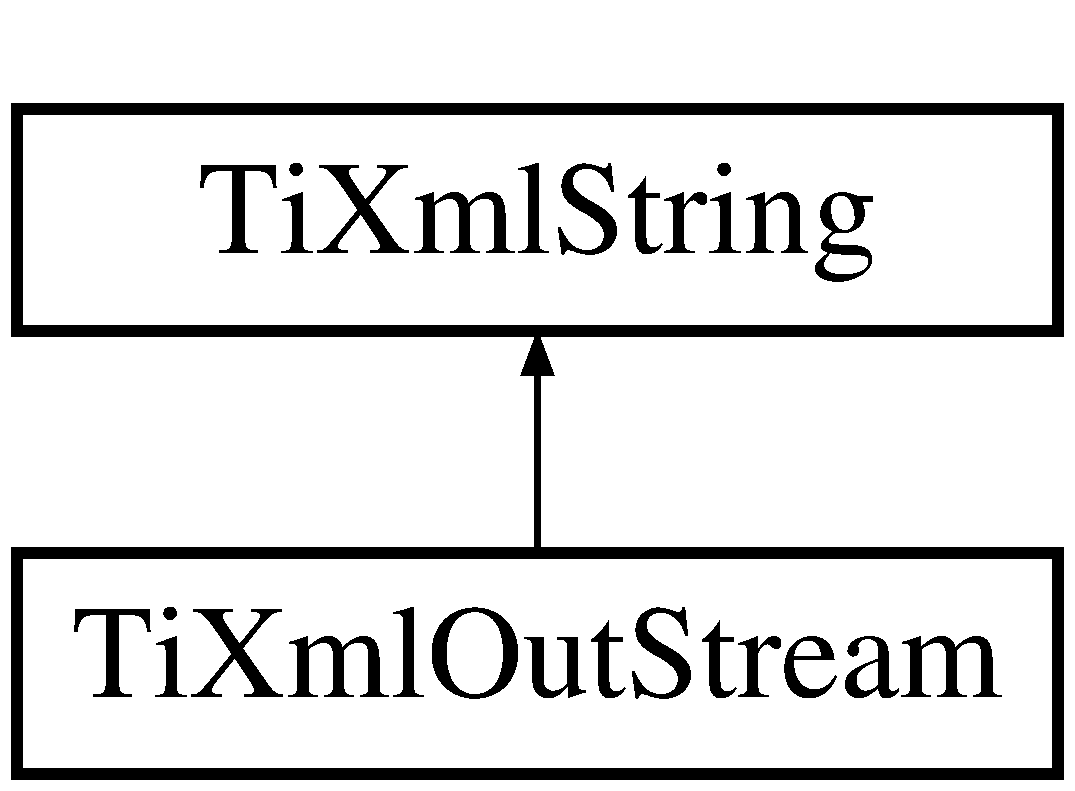
\includegraphics[height=2.000000cm]{class_ti_xml_out_stream}
\end{center}
\end{figure}
\subsection*{Public Member Functions}
\begin{DoxyCompactItemize}
\item 
\hypertarget{class_ti_xml_out_stream_a3640dcb1c0903be3bc6966cdc9a79db6}{\hyperlink{class_ti_xml_out_stream}{Ti\+Xml\+Out\+Stream} \& {\bfseries operator$<$$<$} (const \hyperlink{class_ti_xml_string}{Ti\+Xml\+String} \&in)}\label{class_ti_xml_out_stream_a3640dcb1c0903be3bc6966cdc9a79db6}

\item 
\hypertarget{class_ti_xml_out_stream_af2117e5a8cbfcb69544804ad2859bfb6}{\hyperlink{class_ti_xml_out_stream}{Ti\+Xml\+Out\+Stream} \& {\bfseries operator$<$$<$} (const char $\ast$in)}\label{class_ti_xml_out_stream_af2117e5a8cbfcb69544804ad2859bfb6}

\end{DoxyCompactItemize}
\subsection*{Additional Inherited Members}


The documentation for this class was generated from the following file\+:\begin{DoxyCompactItemize}
\item 
C\+:/\+Users/\+Avenger/\+Documents/\+Git\+Hub/\+Projet-\/\+Tamagoshi/includes/tinyxml/tinystr.\+h\end{DoxyCompactItemize}

\hypertarget{class_ti_xml_parsing_data}{\section{Ti\+Xml\+Parsing\+Data Class Reference}
\label{class_ti_xml_parsing_data}\index{Ti\+Xml\+Parsing\+Data@{Ti\+Xml\+Parsing\+Data}}
}
\subsection*{Public Member Functions}
\begin{DoxyCompactItemize}
\item 
\hypertarget{class_ti_xml_parsing_data_a65cee8ab77a36c605db08c84b4c30a7d}{void {\bfseries Stamp} (const char $\ast$now, Ti\+Xml\+Encoding encoding)}\label{class_ti_xml_parsing_data_a65cee8ab77a36c605db08c84b4c30a7d}

\item 
\hypertarget{class_ti_xml_parsing_data_a9e63d965fdb53ff4ac711e105269e918}{const \hyperlink{struct_ti_xml_cursor}{Ti\+Xml\+Cursor} \& {\bfseries Cursor} () const }\label{class_ti_xml_parsing_data_a9e63d965fdb53ff4ac711e105269e918}

\end{DoxyCompactItemize}
\subsection*{Friends}
\begin{DoxyCompactItemize}
\item 
\hypertarget{class_ti_xml_parsing_data_a173617f6dfe902cf484ce5552b950475}{class {\bfseries Ti\+Xml\+Document}}\label{class_ti_xml_parsing_data_a173617f6dfe902cf484ce5552b950475}

\end{DoxyCompactItemize}


The documentation for this class was generated from the following file\+:\begin{DoxyCompactItemize}
\item 
C\+:/\+Users/\+Avenger/\+Documents/\+Git\+Hub/\+Projet-\/\+Tamagoshi/includes/tinyxml/tinyxmlparser.\+cpp\end{DoxyCompactItemize}

\hypertarget{class_ti_xml_printer}{\section{Ti\+Xml\+Printer Class Reference}
\label{class_ti_xml_printer}\index{Ti\+Xml\+Printer@{Ti\+Xml\+Printer}}
}


{\ttfamily \#include $<$tinyxml.\+h$>$}

Inheritance diagram for Ti\+Xml\+Printer\+:\begin{figure}[H]
\begin{center}
\leavevmode
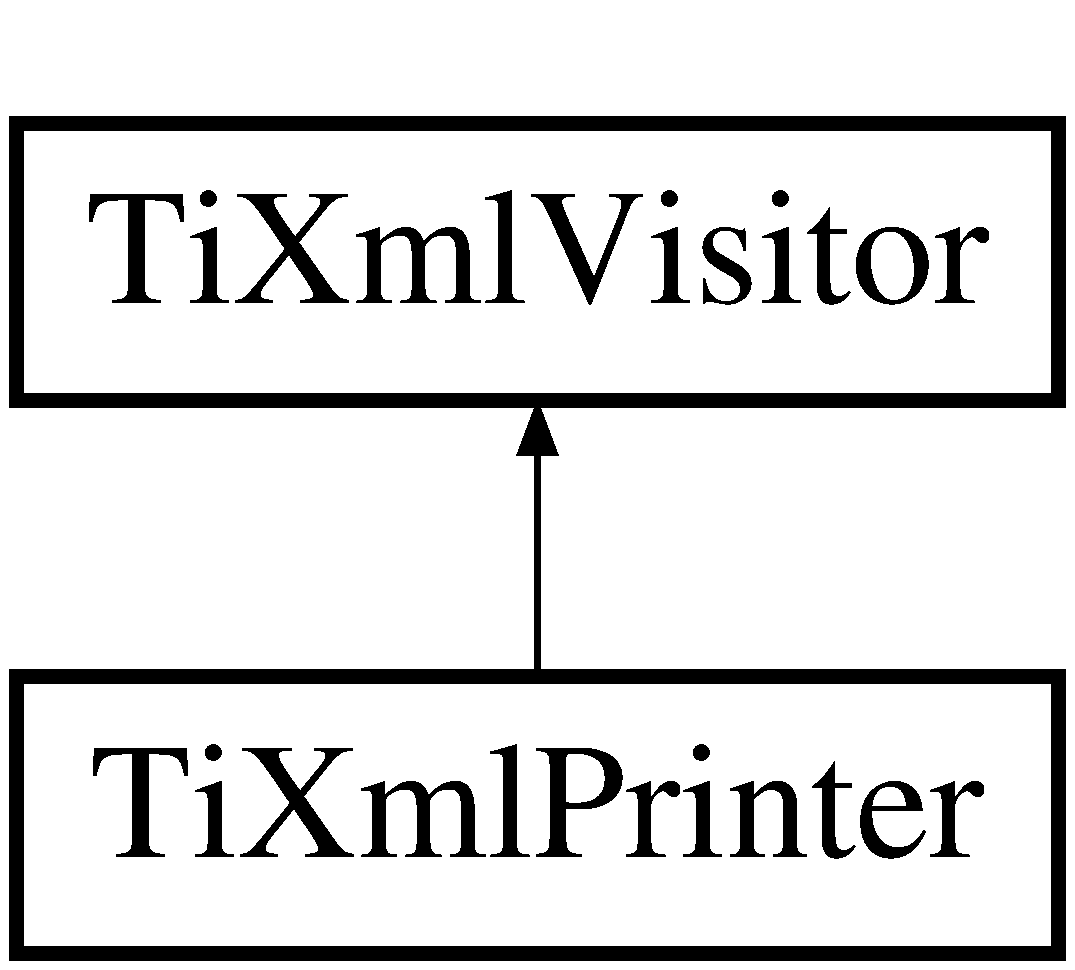
\includegraphics[height=2.000000cm]{class_ti_xml_printer}
\end{center}
\end{figure}
\subsection*{Public Member Functions}
\begin{DoxyCompactItemize}
\item 
\hypertarget{class_ti_xml_printer_a2ec73087db26ff4d2c4316c56f861db7}{virtual bool \hyperlink{class_ti_xml_printer_a2ec73087db26ff4d2c4316c56f861db7}{Visit\+Enter} (const \hyperlink{class_ti_xml_document}{Ti\+Xml\+Document} \&doc)}\label{class_ti_xml_printer_a2ec73087db26ff4d2c4316c56f861db7}

\begin{DoxyCompactList}\small\item\em Visit a document. \end{DoxyCompactList}\item 
\hypertarget{class_ti_xml_printer_a0a636046fa589b6d7f3e5bd025b3f33e}{virtual bool \hyperlink{class_ti_xml_printer_a0a636046fa589b6d7f3e5bd025b3f33e}{Visit\+Exit} (const \hyperlink{class_ti_xml_document}{Ti\+Xml\+Document} \&doc)}\label{class_ti_xml_printer_a0a636046fa589b6d7f3e5bd025b3f33e}

\begin{DoxyCompactList}\small\item\em Visit a document. \end{DoxyCompactList}\item 
\hypertarget{class_ti_xml_printer_a6dccaf5ee4979f13877690afe28721e8}{virtual bool \hyperlink{class_ti_xml_printer_a6dccaf5ee4979f13877690afe28721e8}{Visit\+Enter} (const \hyperlink{class_ti_xml_element}{Ti\+Xml\+Element} \&element, const \hyperlink{class_ti_xml_attribute}{Ti\+Xml\+Attribute} $\ast$first\+Attribute)}\label{class_ti_xml_printer_a6dccaf5ee4979f13877690afe28721e8}

\begin{DoxyCompactList}\small\item\em Visit an element. \end{DoxyCompactList}\item 
\hypertarget{class_ti_xml_printer_ae6a1df8271df4bf62d7873c38e34aa69}{virtual bool \hyperlink{class_ti_xml_printer_ae6a1df8271df4bf62d7873c38e34aa69}{Visit\+Exit} (const \hyperlink{class_ti_xml_element}{Ti\+Xml\+Element} \&element)}\label{class_ti_xml_printer_ae6a1df8271df4bf62d7873c38e34aa69}

\begin{DoxyCompactList}\small\item\em Visit an element. \end{DoxyCompactList}\item 
\hypertarget{class_ti_xml_printer_adaf7eec4dc43ad071ff52b60361574f5}{virtual bool \hyperlink{class_ti_xml_printer_adaf7eec4dc43ad071ff52b60361574f5}{Visit} (const \hyperlink{class_ti_xml_declaration}{Ti\+Xml\+Declaration} \&declaration)}\label{class_ti_xml_printer_adaf7eec4dc43ad071ff52b60361574f5}

\begin{DoxyCompactList}\small\item\em Visit a declaration. \end{DoxyCompactList}\item 
\hypertarget{class_ti_xml_printer_a0857c5d32c59b9a257f9a49cb9411df5}{virtual bool \hyperlink{class_ti_xml_printer_a0857c5d32c59b9a257f9a49cb9411df5}{Visit} (const \hyperlink{class_ti_xml_text}{Ti\+Xml\+Text} \&text)}\label{class_ti_xml_printer_a0857c5d32c59b9a257f9a49cb9411df5}

\begin{DoxyCompactList}\small\item\em Visit a text node. \end{DoxyCompactList}\item 
\hypertarget{class_ti_xml_printer_a9870423f5603630e6142f6bdb66dfb57}{virtual bool \hyperlink{class_ti_xml_printer_a9870423f5603630e6142f6bdb66dfb57}{Visit} (const \hyperlink{class_ti_xml_comment}{Ti\+Xml\+Comment} \&comment)}\label{class_ti_xml_printer_a9870423f5603630e6142f6bdb66dfb57}

\begin{DoxyCompactList}\small\item\em Visit a comment node. \end{DoxyCompactList}\item 
\hypertarget{class_ti_xml_printer_a08591a15c9a07afa83c24e08b03d6358}{virtual bool \hyperlink{class_ti_xml_printer_a08591a15c9a07afa83c24e08b03d6358}{Visit} (const \hyperlink{class_ti_xml_unknown}{Ti\+Xml\+Unknown} \&unknown)}\label{class_ti_xml_printer_a08591a15c9a07afa83c24e08b03d6358}

\begin{DoxyCompactList}\small\item\em Visit an unknown node. \end{DoxyCompactList}\item 
void \hyperlink{class_ti_xml_printer_a213377a4070c7e625bae59716b089e5e}{Set\+Indent} (const char $\ast$\+\_\+indent)
\item 
\hypertarget{class_ti_xml_printer_abb33ec7d4bad6aaeb57f4304394b133d}{const char $\ast$ \hyperlink{class_ti_xml_printer_abb33ec7d4bad6aaeb57f4304394b133d}{Indent} ()}\label{class_ti_xml_printer_abb33ec7d4bad6aaeb57f4304394b133d}

\begin{DoxyCompactList}\small\item\em Query the indention string. \end{DoxyCompactList}\item 
void \hyperlink{class_ti_xml_printer_a4be1e37e69e3858c59635aa947174fe6}{Set\+Line\+Break} (const char $\ast$\+\_\+line\+Break)
\item 
\hypertarget{class_ti_xml_printer_a11f1b4804a460b175ec244eb5724d96d}{const char $\ast$ \hyperlink{class_ti_xml_printer_a11f1b4804a460b175ec244eb5724d96d}{Line\+Break} ()}\label{class_ti_xml_printer_a11f1b4804a460b175ec244eb5724d96d}

\begin{DoxyCompactList}\small\item\em Query the current line breaking string. \end{DoxyCompactList}\item 
void \hyperlink{class_ti_xml_printer_ab23a90629e374cb1cadca090468bbd19}{Set\+Stream\+Printing} ()
\item 
\hypertarget{class_ti_xml_printer_a859eede9597d3e0355b77757be48735e}{const char $\ast$ \hyperlink{class_ti_xml_printer_a859eede9597d3e0355b77757be48735e}{C\+Str} ()}\label{class_ti_xml_printer_a859eede9597d3e0355b77757be48735e}

\begin{DoxyCompactList}\small\item\em Return the result. \end{DoxyCompactList}\item 
\hypertarget{class_ti_xml_printer_ad01375ae9199bd2f48252eaddce3039d}{size\+\_\+t \hyperlink{class_ti_xml_printer_ad01375ae9199bd2f48252eaddce3039d}{Size} ()}\label{class_ti_xml_printer_ad01375ae9199bd2f48252eaddce3039d}

\begin{DoxyCompactList}\small\item\em Return the length of the result string. \end{DoxyCompactList}\item 
\hypertarget{class_ti_xml_printer_a3bd4daf44309b41f5813a833caa0d1c9}{const std\+::string \& \hyperlink{class_ti_xml_printer_a3bd4daf44309b41f5813a833caa0d1c9}{Str} ()}\label{class_ti_xml_printer_a3bd4daf44309b41f5813a833caa0d1c9}

\begin{DoxyCompactList}\small\item\em Return the result. \end{DoxyCompactList}\end{DoxyCompactItemize}


\subsection{Detailed Description}
Print to memory functionality. The \hyperlink{class_ti_xml_printer}{Ti\+Xml\+Printer} is useful when you need to\+:


\begin{DoxyEnumerate}
\item Print to memory (especially in non-\/\+S\+T\+L mode)
\item Control formatting (line endings, etc.)
\end{DoxyEnumerate}

When constructed, the \hyperlink{class_ti_xml_printer}{Ti\+Xml\+Printer} is in its default \char`\"{}pretty printing\char`\"{} mode. Before calling Accept() you can call methods to control the printing of the X\+M\+L document. After \hyperlink{class_ti_xml_node_acc0f88b7462c6cb73809d410a4f5bb86}{Ti\+Xml\+Node\+::\+Accept()} is called, the printed document can be accessed via the \hyperlink{class_ti_xml_printer_a859eede9597d3e0355b77757be48735e}{C\+Str()}, \hyperlink{class_ti_xml_printer_a3bd4daf44309b41f5813a833caa0d1c9}{Str()}, and \hyperlink{class_ti_xml_printer_ad01375ae9199bd2f48252eaddce3039d}{Size()} methods.

\hyperlink{class_ti_xml_printer}{Ti\+Xml\+Printer} uses the Visitor A\+P\+I. \begin{DoxyVerb}TiXmlPrinter printer;
printer.SetIndent( "\t" );

doc.Accept( &printer );
fprintf( stdout, "%s", printer.CStr() );
\end{DoxyVerb}
 

\subsection{Member Function Documentation}
\hypertarget{class_ti_xml_printer_a213377a4070c7e625bae59716b089e5e}{\index{Ti\+Xml\+Printer@{Ti\+Xml\+Printer}!Set\+Indent@{Set\+Indent}}
\index{Set\+Indent@{Set\+Indent}!Ti\+Xml\+Printer@{Ti\+Xml\+Printer}}
\subsubsection[{Set\+Indent}]{\setlength{\rightskip}{0pt plus 5cm}void Ti\+Xml\+Printer\+::\+Set\+Indent (
\begin{DoxyParamCaption}
\item[{const char $\ast$}]{\+\_\+indent}
\end{DoxyParamCaption}
)\hspace{0.3cm}{\ttfamily [inline]}}}\label{class_ti_xml_printer_a213377a4070c7e625bae59716b089e5e}
Set the indent characters for printing. By default 4 spaces but tab () is also useful, or null/empty string for no indentation. \hypertarget{class_ti_xml_printer_a4be1e37e69e3858c59635aa947174fe6}{\index{Ti\+Xml\+Printer@{Ti\+Xml\+Printer}!Set\+Line\+Break@{Set\+Line\+Break}}
\index{Set\+Line\+Break@{Set\+Line\+Break}!Ti\+Xml\+Printer@{Ti\+Xml\+Printer}}
\subsubsection[{Set\+Line\+Break}]{\setlength{\rightskip}{0pt plus 5cm}void Ti\+Xml\+Printer\+::\+Set\+Line\+Break (
\begin{DoxyParamCaption}
\item[{const char $\ast$}]{\+\_\+line\+Break}
\end{DoxyParamCaption}
)\hspace{0.3cm}{\ttfamily [inline]}}}\label{class_ti_xml_printer_a4be1e37e69e3858c59635aa947174fe6}
Set the line breaking string. By default set to newline (~\newline
). Some operating systems prefer other characters, or can be set to the null/empty string for no indenation. \hypertarget{class_ti_xml_printer_ab23a90629e374cb1cadca090468bbd19}{\index{Ti\+Xml\+Printer@{Ti\+Xml\+Printer}!Set\+Stream\+Printing@{Set\+Stream\+Printing}}
\index{Set\+Stream\+Printing@{Set\+Stream\+Printing}!Ti\+Xml\+Printer@{Ti\+Xml\+Printer}}
\subsubsection[{Set\+Stream\+Printing}]{\setlength{\rightskip}{0pt plus 5cm}void Ti\+Xml\+Printer\+::\+Set\+Stream\+Printing (
\begin{DoxyParamCaption}
{}
\end{DoxyParamCaption}
)\hspace{0.3cm}{\ttfamily [inline]}}}\label{class_ti_xml_printer_ab23a90629e374cb1cadca090468bbd19}
Switch over to \char`\"{}stream printing\char`\"{} which is the most dense formatting without linebreaks. Common when the X\+M\+L is needed for network transmission. 

The documentation for this class was generated from the following files\+:\begin{DoxyCompactItemize}
\item 
C\+:/\+Users/\+Avenger/\+Documents/\+Git\+Hub/\+Projet-\/\+Tamagoshi/includes/tinyxml/tinyxml.\+h\item 
C\+:/\+Users/\+Avenger/\+Documents/\+Git\+Hub/\+Projet-\/\+Tamagoshi/includes/tinyxml/tinyxml.\+cpp\end{DoxyCompactItemize}

\hypertarget{class_ti_xml_string}{\section{Ti\+Xml\+String Class Reference}
\label{class_ti_xml_string}\index{Ti\+Xml\+String@{Ti\+Xml\+String}}
}
Inheritance diagram for Ti\+Xml\+String\+:\begin{figure}[H]
\begin{center}
\leavevmode
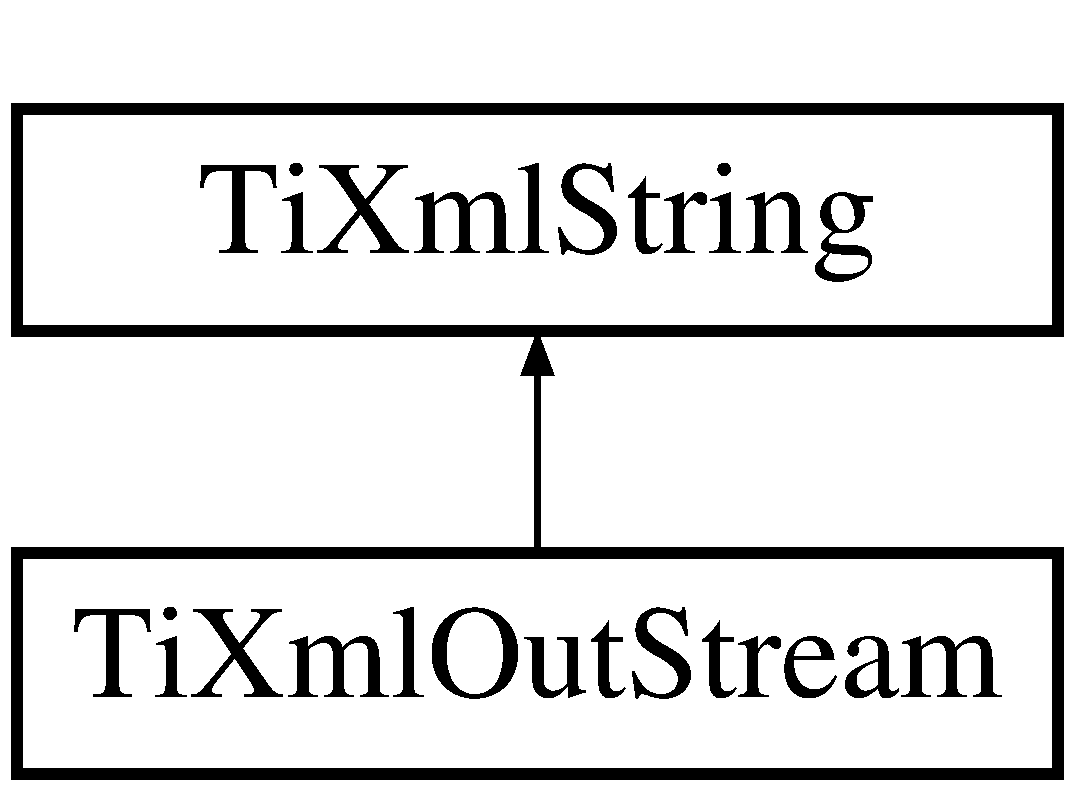
\includegraphics[height=2.000000cm]{class_ti_xml_string}
\end{center}
\end{figure}
\subsection*{Public Types}
\begin{DoxyCompactItemize}
\item 
\hypertarget{class_ti_xml_string_abeb2c1893a04c17904f7c06546d0b971}{typedef size\+\_\+t {\bfseries size\+\_\+type}}\label{class_ti_xml_string_abeb2c1893a04c17904f7c06546d0b971}

\end{DoxyCompactItemize}
\subsection*{Public Member Functions}
\begin{DoxyCompactItemize}
\item 
\hypertarget{class_ti_xml_string_ac80fe17693a438c9ab2591664743fcb6}{{\bfseries Ti\+Xml\+String} (const \hyperlink{class_ti_xml_string}{Ti\+Xml\+String} \&copy)}\label{class_ti_xml_string_ac80fe17693a438c9ab2591664743fcb6}

\item 
\hypertarget{class_ti_xml_string_aa3b32bd2891a757c9f36c21db44c81d2}{T\+I\+X\+M\+L\+\_\+\+E\+X\+P\+L\+I\+C\+I\+T {\bfseries Ti\+Xml\+String} (const char $\ast$copy)}\label{class_ti_xml_string_aa3b32bd2891a757c9f36c21db44c81d2}

\item 
\hypertarget{class_ti_xml_string_a4b17ea5c5db986f14827223dfa8f1547}{T\+I\+X\+M\+L\+\_\+\+E\+X\+P\+L\+I\+C\+I\+T {\bfseries Ti\+Xml\+String} (const char $\ast$str, size\+\_\+type len)}\label{class_ti_xml_string_a4b17ea5c5db986f14827223dfa8f1547}

\item 
\hypertarget{class_ti_xml_string_ae0bc6147afc0ec2aa0da3a3c0a8fcfb0}{\hyperlink{class_ti_xml_string}{Ti\+Xml\+String} \& {\bfseries operator=} (const char $\ast$copy)}\label{class_ti_xml_string_ae0bc6147afc0ec2aa0da3a3c0a8fcfb0}

\item 
\hypertarget{class_ti_xml_string_ab1f1f5d3eceaa0f22d0a7e6055ea81b0}{\hyperlink{class_ti_xml_string}{Ti\+Xml\+String} \& {\bfseries operator=} (const \hyperlink{class_ti_xml_string}{Ti\+Xml\+String} \&copy)}\label{class_ti_xml_string_ab1f1f5d3eceaa0f22d0a7e6055ea81b0}

\item 
\hypertarget{class_ti_xml_string_ab56336ac2aa2a08d24a71eb9a2b502a5}{\hyperlink{class_ti_xml_string}{Ti\+Xml\+String} \& {\bfseries operator+=} (const char $\ast$suffix)}\label{class_ti_xml_string_ab56336ac2aa2a08d24a71eb9a2b502a5}

\item 
\hypertarget{class_ti_xml_string_a6aa09d5240470b76d54ec709e04f8c13}{\hyperlink{class_ti_xml_string}{Ti\+Xml\+String} \& {\bfseries operator+=} (char single)}\label{class_ti_xml_string_a6aa09d5240470b76d54ec709e04f8c13}

\item 
\hypertarget{class_ti_xml_string_afdcae5ea2b4d9e194dc21226b817f417}{\hyperlink{class_ti_xml_string}{Ti\+Xml\+String} \& {\bfseries operator+=} (const \hyperlink{class_ti_xml_string}{Ti\+Xml\+String} \&suffix)}\label{class_ti_xml_string_afdcae5ea2b4d9e194dc21226b817f417}

\item 
\hypertarget{class_ti_xml_string_a5581ca641d915551d3cda90f8e7bf49b}{const char $\ast$ {\bfseries c\+\_\+str} () const }\label{class_ti_xml_string_a5581ca641d915551d3cda90f8e7bf49b}

\item 
\hypertarget{class_ti_xml_string_a00abc60f135c7ca1951c7334cc2c7993}{const char $\ast$ {\bfseries data} () const }\label{class_ti_xml_string_a00abc60f135c7ca1951c7334cc2c7993}

\item 
\hypertarget{class_ti_xml_string_a3202f27d139a3fac79205f1f3c707727}{size\+\_\+type {\bfseries length} () const }\label{class_ti_xml_string_a3202f27d139a3fac79205f1f3c707727}

\item 
\hypertarget{class_ti_xml_string_a96103e5c0f67e987fa48527e1f47a1f6}{size\+\_\+type {\bfseries size} () const }\label{class_ti_xml_string_a96103e5c0f67e987fa48527e1f47a1f6}

\item 
\hypertarget{class_ti_xml_string_a9a61e1d11cdb71bea4a4ed79caa793f4}{bool {\bfseries empty} () const }\label{class_ti_xml_string_a9a61e1d11cdb71bea4a4ed79caa793f4}

\item 
\hypertarget{class_ti_xml_string_a76e4d6aba7845f4cf9c02332a5fbf916}{size\+\_\+type {\bfseries capacity} () const }\label{class_ti_xml_string_a76e4d6aba7845f4cf9c02332a5fbf916}

\item 
\hypertarget{class_ti_xml_string_a6763093267bbdecbf03f8840bc349877}{const char \& {\bfseries at} (size\+\_\+type index) const }\label{class_ti_xml_string_a6763093267bbdecbf03f8840bc349877}

\item 
\hypertarget{class_ti_xml_string_ae8cdc1d46c538536b786f7ae03c0c1d9}{char \& {\bfseries operator\mbox{[}$\,$\mbox{]}} (size\+\_\+type index) const }\label{class_ti_xml_string_ae8cdc1d46c538536b786f7ae03c0c1d9}

\item 
\hypertarget{class_ti_xml_string_a5c2b368b5eafe075fd9565cbcbd4c2f9}{size\+\_\+type {\bfseries find} (char lookup) const }\label{class_ti_xml_string_a5c2b368b5eafe075fd9565cbcbd4c2f9}

\item 
\hypertarget{class_ti_xml_string_a5f2a6fd565751410b392f249a9786db4}{size\+\_\+type {\bfseries find} (char tofind, size\+\_\+type offset) const }\label{class_ti_xml_string_a5f2a6fd565751410b392f249a9786db4}

\item 
\hypertarget{class_ti_xml_string_ab20e06e4c666abf3bdbfb3a1191d4888}{void {\bfseries clear} ()}\label{class_ti_xml_string_ab20e06e4c666abf3bdbfb3a1191d4888}

\item 
\hypertarget{class_ti_xml_string_a88ecf9f0f00cb5c67b6b637958d7049c}{void {\bfseries reserve} (size\+\_\+type cap)}\label{class_ti_xml_string_a88ecf9f0f00cb5c67b6b637958d7049c}

\item 
\hypertarget{class_ti_xml_string_ac72f3d9149b7812c1e6c59402014d0d5}{\hyperlink{class_ti_xml_string}{Ti\+Xml\+String} \& {\bfseries assign} (const char $\ast$str, size\+\_\+type len)}\label{class_ti_xml_string_ac72f3d9149b7812c1e6c59402014d0d5}

\item 
\hypertarget{class_ti_xml_string_ad44b21700d2ec24a511367b222b643fb}{\hyperlink{class_ti_xml_string}{Ti\+Xml\+String} \& {\bfseries append} (const char $\ast$str, size\+\_\+type len)}\label{class_ti_xml_string_ad44b21700d2ec24a511367b222b643fb}

\item 
\hypertarget{class_ti_xml_string_aa392cbc180752a79f007f4f9280c7762}{void {\bfseries swap} (\hyperlink{class_ti_xml_string}{Ti\+Xml\+String} \&other)}\label{class_ti_xml_string_aa392cbc180752a79f007f4f9280c7762}

\end{DoxyCompactItemize}
\subsection*{Static Public Attributes}
\begin{DoxyCompactItemize}
\item 
\hypertarget{class_ti_xml_string_a8f4422d227088dc7bec96f479b275d0a}{static const size\+\_\+type {\bfseries npos} = static\+\_\+cast$<$ Ti\+Xml\+String\+::size\+\_\+type $>$(-\/1)}\label{class_ti_xml_string_a8f4422d227088dc7bec96f479b275d0a}

\end{DoxyCompactItemize}


The documentation for this class was generated from the following files\+:\begin{DoxyCompactItemize}
\item 
C\+:/\+Users/\+Avenger/\+Documents/\+Git\+Hub/\+Projet-\/\+Tamagoshi/includes/tinyxml/tinystr.\+h\item 
C\+:/\+Users/\+Avenger/\+Documents/\+Git\+Hub/\+Projet-\/\+Tamagoshi/includes/tinyxml/tinystr.\+cpp\end{DoxyCompactItemize}

\hypertarget{class_ti_xml_text}{\section{Ti\+Xml\+Text Class Reference}
\label{class_ti_xml_text}\index{Ti\+Xml\+Text@{Ti\+Xml\+Text}}
}


{\ttfamily \#include $<$tinyxml.\+h$>$}

Inheritance diagram for Ti\+Xml\+Text\+:\begin{figure}[H]
\begin{center}
\leavevmode
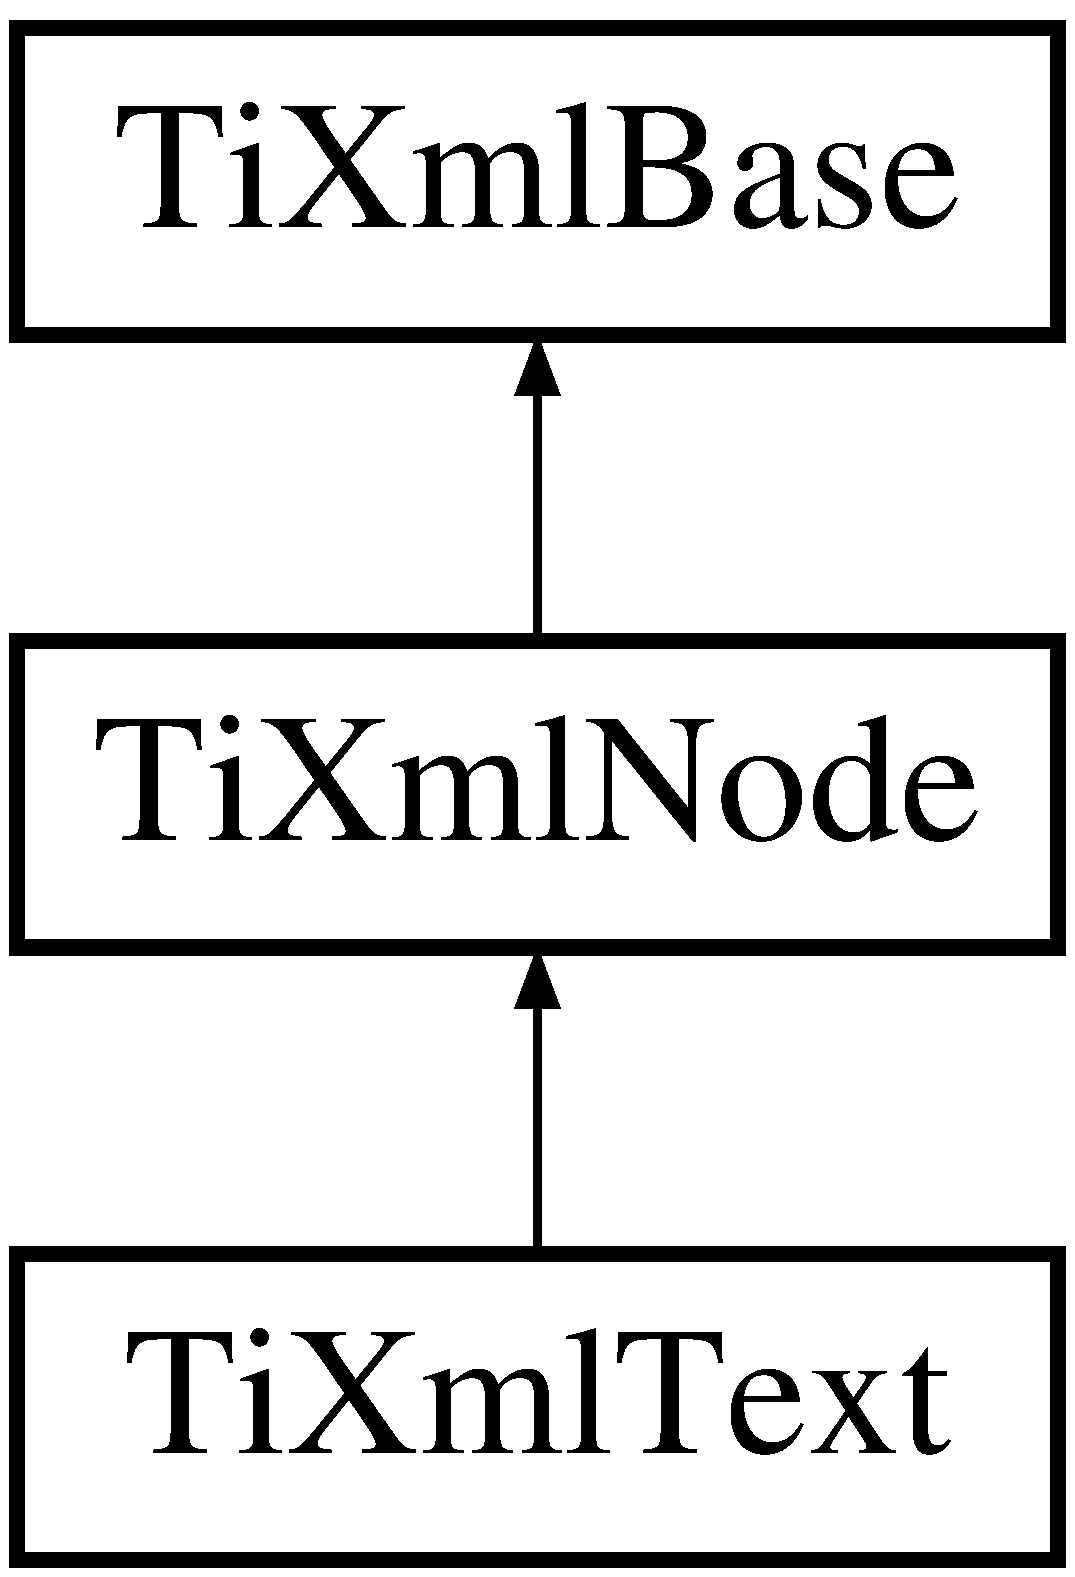
\includegraphics[height=3.000000cm]{class_ti_xml_text}
\end{center}
\end{figure}
\subsection*{Public Member Functions}
\begin{DoxyCompactItemize}
\item 
\hyperlink{class_ti_xml_text_af659e77c6b87d684827f35a8f4895960}{Ti\+Xml\+Text} (const char $\ast$init\+Value)
\item 
\hypertarget{class_ti_xml_text_a439792f6183a3d3fb6f2bc2b16fa5691}{\hyperlink{class_ti_xml_text_a439792f6183a3d3fb6f2bc2b16fa5691}{Ti\+Xml\+Text} (const std\+::string \&init\+Value)}\label{class_ti_xml_text_a439792f6183a3d3fb6f2bc2b16fa5691}

\begin{DoxyCompactList}\small\item\em Constructor. \end{DoxyCompactList}\item 
\hypertarget{class_ti_xml_text_a8d2cc1b4af2208cbb0171cf20f6815d1}{{\bfseries Ti\+Xml\+Text} (const \hyperlink{class_ti_xml_text}{Ti\+Xml\+Text} \&copy)}\label{class_ti_xml_text_a8d2cc1b4af2208cbb0171cf20f6815d1}

\item 
\hypertarget{class_ti_xml_text_aed5b13f9c1b804c616fd533882c29f57}{\hyperlink{class_ti_xml_text}{Ti\+Xml\+Text} \& {\bfseries operator=} (const \hyperlink{class_ti_xml_text}{Ti\+Xml\+Text} \&base)}\label{class_ti_xml_text_aed5b13f9c1b804c616fd533882c29f57}

\item 
virtual void \hyperlink{class_ti_xml_text_ae74d56c5b3ddec6cc3103dd51821af92}{Print} (F\+I\+L\+E $\ast$cfile, int depth) const 
\item 
\hypertarget{class_ti_xml_text_ad1a6a6b83fa2271022dd97c072a2b586}{bool \hyperlink{class_ti_xml_text_ad1a6a6b83fa2271022dd97c072a2b586}{C\+D\+A\+T\+A} () const }\label{class_ti_xml_text_ad1a6a6b83fa2271022dd97c072a2b586}

\begin{DoxyCompactList}\small\item\em Queries whether this represents text using a C\+D\+A\+T\+A section. \end{DoxyCompactList}\item 
\hypertarget{class_ti_xml_text_acb17ff7c5d09b2c839393445a3de5ea9}{void \hyperlink{class_ti_xml_text_acb17ff7c5d09b2c839393445a3de5ea9}{Set\+C\+D\+A\+T\+A} (bool \+\_\+cdata)}\label{class_ti_xml_text_acb17ff7c5d09b2c839393445a3de5ea9}

\begin{DoxyCompactList}\small\item\em Turns on or off a C\+D\+A\+T\+A representation of text. \end{DoxyCompactList}\item 
\hypertarget{class_ti_xml_text_a8d2dcfa41fc73d3e62dacc2fcf633819}{virtual const char $\ast$ {\bfseries Parse} (const char $\ast$p, \hyperlink{class_ti_xml_parsing_data}{Ti\+Xml\+Parsing\+Data} $\ast$data, Ti\+Xml\+Encoding encoding)}\label{class_ti_xml_text_a8d2dcfa41fc73d3e62dacc2fcf633819}

\item 
\hypertarget{class_ti_xml_text_a895bf34ffad17f7439ab2a52b9651648}{virtual const \hyperlink{class_ti_xml_text}{Ti\+Xml\+Text} $\ast$ \hyperlink{class_ti_xml_text_a895bf34ffad17f7439ab2a52b9651648}{To\+Text} () const }\label{class_ti_xml_text_a895bf34ffad17f7439ab2a52b9651648}

\begin{DoxyCompactList}\small\item\em Cast to a more defined type. Will return null not of the requested type. \end{DoxyCompactList}\item 
\hypertarget{class_ti_xml_text_ae7c3a8fd3e4dbf6c0c4363a943d72f5b}{virtual \hyperlink{class_ti_xml_text}{Ti\+Xml\+Text} $\ast$ \hyperlink{class_ti_xml_text_ae7c3a8fd3e4dbf6c0c4363a943d72f5b}{To\+Text} ()}\label{class_ti_xml_text_ae7c3a8fd3e4dbf6c0c4363a943d72f5b}

\begin{DoxyCompactList}\small\item\em Cast to a more defined type. Will return null not of the requested type. \end{DoxyCompactList}\item 
virtual bool \hyperlink{class_ti_xml_text_a43b9954ebf679557fac1a4453f337b7c}{Accept} (\hyperlink{class_ti_xml_visitor}{Ti\+Xml\+Visitor} $\ast$content) const 
\end{DoxyCompactItemize}
\subsection*{Protected Member Functions}
\begin{DoxyCompactItemize}
\item 
\hypertarget{class_ti_xml_text_adde1869dfb029be50713fbfd8ce4d21f}{virtual \hyperlink{class_ti_xml_node}{Ti\+Xml\+Node} $\ast$ \hyperlink{class_ti_xml_text_adde1869dfb029be50713fbfd8ce4d21f}{Clone} () const }\label{class_ti_xml_text_adde1869dfb029be50713fbfd8ce4d21f}

\begin{DoxyCompactList}\small\item\em \mbox{[}internal use\mbox{]} Creates a new Element and returns it. \end{DoxyCompactList}\item 
\hypertarget{class_ti_xml_text_adcec7d9b6fccfc5777452bb97e6031c1}{void {\bfseries Copy\+To} (\hyperlink{class_ti_xml_text}{Ti\+Xml\+Text} $\ast$target) const }\label{class_ti_xml_text_adcec7d9b6fccfc5777452bb97e6031c1}

\item 
\hypertarget{class_ti_xml_text_a1c120428e3b3cf24d79706e6d2b65aa6}{bool {\bfseries Blank} () const }\label{class_ti_xml_text_a1c120428e3b3cf24d79706e6d2b65aa6}

\item 
\hypertarget{class_ti_xml_text_a261e07cdbd5363f994371320414c17d9}{virtual void {\bfseries Stream\+In} (std\+::istream $\ast$in, T\+I\+X\+M\+L\+\_\+\+S\+T\+R\+I\+N\+G $\ast$tag)}\label{class_ti_xml_text_a261e07cdbd5363f994371320414c17d9}

\end{DoxyCompactItemize}
\subsection*{Friends}
\begin{DoxyCompactItemize}
\item 
\hypertarget{class_ti_xml_text_ab6592e32cb9132be517cc12a70564c4b}{class {\bfseries Ti\+Xml\+Element}}\label{class_ti_xml_text_ab6592e32cb9132be517cc12a70564c4b}

\end{DoxyCompactItemize}
\subsection*{Additional Inherited Members}


\subsection{Detailed Description}
X\+M\+L text. A text node can have 2 ways to output the next. \char`\"{}normal\char`\"{} output and C\+D\+A\+T\+A. It will default to the mode it was parsed from the X\+M\+L file and you generally want to leave it alone, but you can change the output mode with \hyperlink{class_ti_xml_text_acb17ff7c5d09b2c839393445a3de5ea9}{Set\+C\+D\+A\+T\+A()} and query it with \hyperlink{class_ti_xml_text_ad1a6a6b83fa2271022dd97c072a2b586}{C\+D\+A\+T\+A()}. 

\subsection{Constructor \& Destructor Documentation}
\hypertarget{class_ti_xml_text_af659e77c6b87d684827f35a8f4895960}{\index{Ti\+Xml\+Text@{Ti\+Xml\+Text}!Ti\+Xml\+Text@{Ti\+Xml\+Text}}
\index{Ti\+Xml\+Text@{Ti\+Xml\+Text}!Ti\+Xml\+Text@{Ti\+Xml\+Text}}
\subsubsection[{Ti\+Xml\+Text}]{\setlength{\rightskip}{0pt plus 5cm}Ti\+Xml\+Text\+::\+Ti\+Xml\+Text (
\begin{DoxyParamCaption}
\item[{const char $\ast$}]{init\+Value}
\end{DoxyParamCaption}
)\hspace{0.3cm}{\ttfamily [inline]}}}\label{class_ti_xml_text_af659e77c6b87d684827f35a8f4895960}
Constructor for text element. By default, it is treated as normal, encoded text. If you want it be output as a C\+D\+A\+T\+A text element, set the parameter \+\_\+cdata to 'true' 

\subsection{Member Function Documentation}
\hypertarget{class_ti_xml_text_a43b9954ebf679557fac1a4453f337b7c}{\index{Ti\+Xml\+Text@{Ti\+Xml\+Text}!Accept@{Accept}}
\index{Accept@{Accept}!Ti\+Xml\+Text@{Ti\+Xml\+Text}}
\subsubsection[{Accept}]{\setlength{\rightskip}{0pt plus 5cm}bool Ti\+Xml\+Text\+::\+Accept (
\begin{DoxyParamCaption}
\item[{{\bf Ti\+Xml\+Visitor} $\ast$}]{content}
\end{DoxyParamCaption}
) const\hspace{0.3cm}{\ttfamily [virtual]}}}\label{class_ti_xml_text_a43b9954ebf679557fac1a4453f337b7c}
Walk the X\+M\+L tree visiting this node and all of its children. 

Implements \hyperlink{class_ti_xml_node_acc0f88b7462c6cb73809d410a4f5bb86}{Ti\+Xml\+Node}.

\hypertarget{class_ti_xml_text_ae74d56c5b3ddec6cc3103dd51821af92}{\index{Ti\+Xml\+Text@{Ti\+Xml\+Text}!Print@{Print}}
\index{Print@{Print}!Ti\+Xml\+Text@{Ti\+Xml\+Text}}
\subsubsection[{Print}]{\setlength{\rightskip}{0pt plus 5cm}void Ti\+Xml\+Text\+::\+Print (
\begin{DoxyParamCaption}
\item[{F\+I\+L\+E $\ast$}]{cfile, }
\item[{int}]{depth}
\end{DoxyParamCaption}
) const\hspace{0.3cm}{\ttfamily [virtual]}}}\label{class_ti_xml_text_ae74d56c5b3ddec6cc3103dd51821af92}
All Tiny\+Xml classes can print themselves to a filestream or the string class (\hyperlink{class_ti_xml_string}{Ti\+Xml\+String} in non-\/\+S\+T\+L mode, std\+::string in S\+T\+L mode.) Either or both cfile and str can be null.

This is a formatted print, and will insert tabs and newlines.

(For an unformatted stream, use the $<$$<$ operator.) 

Implements \hyperlink{class_ti_xml_base_a0de56b3f2ef14c65091a3b916437b512}{Ti\+Xml\+Base}.



The documentation for this class was generated from the following files\+:\begin{DoxyCompactItemize}
\item 
C\+:/\+Users/\+Avenger/\+Documents/\+Git\+Hub/\+Projet-\/\+Tamagoshi/includes/tinyxml/tinyxml.\+h\item 
C\+:/\+Users/\+Avenger/\+Documents/\+Git\+Hub/\+Projet-\/\+Tamagoshi/includes/tinyxml/tinyxml.\+cpp\item 
C\+:/\+Users/\+Avenger/\+Documents/\+Git\+Hub/\+Projet-\/\+Tamagoshi/includes/tinyxml/tinyxmlparser.\+cpp\end{DoxyCompactItemize}

\hypertarget{class_ti_xml_unknown}{\section{Ti\+Xml\+Unknown Class Reference}
\label{class_ti_xml_unknown}\index{Ti\+Xml\+Unknown@{Ti\+Xml\+Unknown}}
}


{\ttfamily \#include $<$tinyxml.\+h$>$}

Inheritance diagram for Ti\+Xml\+Unknown\+:\begin{figure}[H]
\begin{center}
\leavevmode
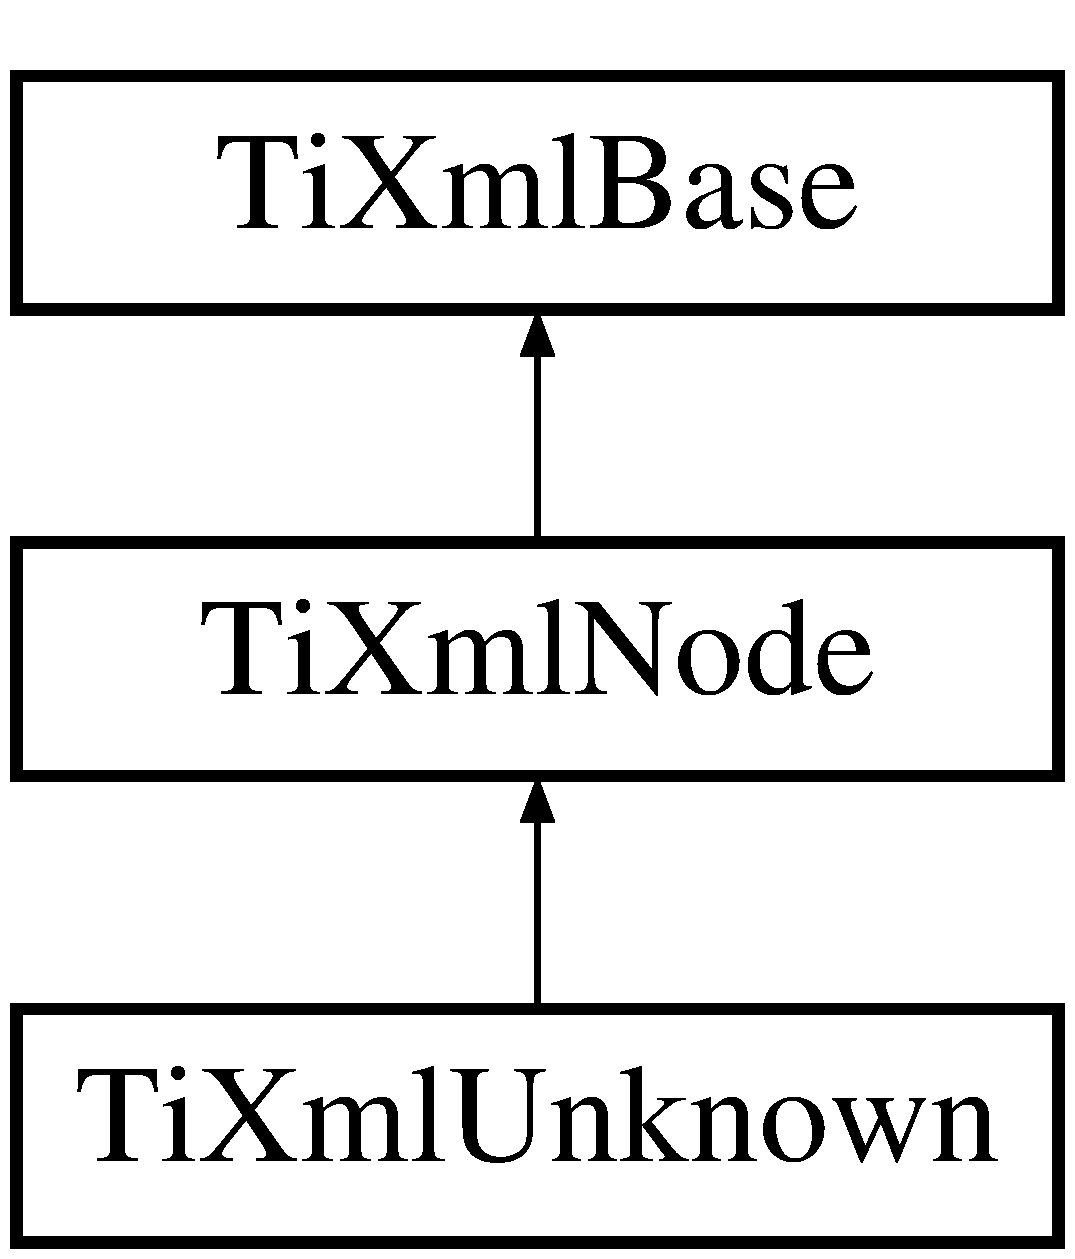
\includegraphics[height=3.000000cm]{class_ti_xml_unknown}
\end{center}
\end{figure}
\subsection*{Public Member Functions}
\begin{DoxyCompactItemize}
\item 
\hypertarget{class_ti_xml_unknown_abe798ff4feea31474850c7f0de6bdf5e}{{\bfseries Ti\+Xml\+Unknown} (const \hyperlink{class_ti_xml_unknown}{Ti\+Xml\+Unknown} \&copy)}\label{class_ti_xml_unknown_abe798ff4feea31474850c7f0de6bdf5e}

\item 
\hypertarget{class_ti_xml_unknown_a60560b5aacb4bdc8b2b5f02f0a99c5c0}{\hyperlink{class_ti_xml_unknown}{Ti\+Xml\+Unknown} \& {\bfseries operator=} (const \hyperlink{class_ti_xml_unknown}{Ti\+Xml\+Unknown} \&copy)}\label{class_ti_xml_unknown_a60560b5aacb4bdc8b2b5f02f0a99c5c0}

\item 
\hypertarget{class_ti_xml_unknown_a675c4b2684af35e4c7649b7fd5ae598d}{virtual \hyperlink{class_ti_xml_node}{Ti\+Xml\+Node} $\ast$ \hyperlink{class_ti_xml_unknown_a675c4b2684af35e4c7649b7fd5ae598d}{Clone} () const }\label{class_ti_xml_unknown_a675c4b2684af35e4c7649b7fd5ae598d}

\begin{DoxyCompactList}\small\item\em Creates a copy of this Unknown and returns it. \end{DoxyCompactList}\item 
virtual void \hyperlink{class_ti_xml_unknown_a025f19c21ef01ea9be50febb8fe0ba06}{Print} (F\+I\+L\+E $\ast$cfile, int depth) const 
\item 
\hypertarget{class_ti_xml_unknown_aa51c2694e4177b5f0b5429ee5a81b58d}{virtual const char $\ast$ {\bfseries Parse} (const char $\ast$p, \hyperlink{class_ti_xml_parsing_data}{Ti\+Xml\+Parsing\+Data} $\ast$data, Ti\+Xml\+Encoding encoding)}\label{class_ti_xml_unknown_aa51c2694e4177b5f0b5429ee5a81b58d}

\item 
\hypertarget{class_ti_xml_unknown_ab0313e5fe77987d746ac1a97a254419d}{virtual const \hyperlink{class_ti_xml_unknown}{Ti\+Xml\+Unknown} $\ast$ \hyperlink{class_ti_xml_unknown_ab0313e5fe77987d746ac1a97a254419d}{To\+Unknown} () const }\label{class_ti_xml_unknown_ab0313e5fe77987d746ac1a97a254419d}

\begin{DoxyCompactList}\small\item\em Cast to a more defined type. Will return null not of the requested type. \end{DoxyCompactList}\item 
\hypertarget{class_ti_xml_unknown_a67c9fd22940e8c47f706a72cdd2e332c}{virtual \hyperlink{class_ti_xml_unknown}{Ti\+Xml\+Unknown} $\ast$ \hyperlink{class_ti_xml_unknown_a67c9fd22940e8c47f706a72cdd2e332c}{To\+Unknown} ()}\label{class_ti_xml_unknown_a67c9fd22940e8c47f706a72cdd2e332c}

\begin{DoxyCompactList}\small\item\em Cast to a more defined type. Will return null not of the requested type. \end{DoxyCompactList}\item 
virtual bool \hyperlink{class_ti_xml_unknown_a4e54d7482e05a837cf83c925cc683380}{Accept} (\hyperlink{class_ti_xml_visitor}{Ti\+Xml\+Visitor} $\ast$content) const 
\end{DoxyCompactItemize}
\subsection*{Protected Member Functions}
\begin{DoxyCompactItemize}
\item 
\hypertarget{class_ti_xml_unknown_a08ca7b225a2bcb604d3c72e199d33408}{void {\bfseries Copy\+To} (\hyperlink{class_ti_xml_unknown}{Ti\+Xml\+Unknown} $\ast$target) const }\label{class_ti_xml_unknown_a08ca7b225a2bcb604d3c72e199d33408}

\item 
\hypertarget{class_ti_xml_unknown_adf84a317816124a2d7c7947d36170458}{virtual void {\bfseries Stream\+In} (std\+::istream $\ast$in, T\+I\+X\+M\+L\+\_\+\+S\+T\+R\+I\+N\+G $\ast$tag)}\label{class_ti_xml_unknown_adf84a317816124a2d7c7947d36170458}

\end{DoxyCompactItemize}
\subsection*{Additional Inherited Members}


\subsection{Detailed Description}
Any tag that tiny\+Xml doesn't recognize is saved as an unknown. It is a tag of text, but should not be modified. It will be written back to the X\+M\+L, unchanged, when the file is saved.

D\+T\+D tags get thrown into Ti\+Xml\+Unknowns. 

\subsection{Member Function Documentation}
\hypertarget{class_ti_xml_unknown_a4e54d7482e05a837cf83c925cc683380}{\index{Ti\+Xml\+Unknown@{Ti\+Xml\+Unknown}!Accept@{Accept}}
\index{Accept@{Accept}!Ti\+Xml\+Unknown@{Ti\+Xml\+Unknown}}
\subsubsection[{Accept}]{\setlength{\rightskip}{0pt plus 5cm}bool Ti\+Xml\+Unknown\+::\+Accept (
\begin{DoxyParamCaption}
\item[{{\bf Ti\+Xml\+Visitor} $\ast$}]{content}
\end{DoxyParamCaption}
) const\hspace{0.3cm}{\ttfamily [virtual]}}}\label{class_ti_xml_unknown_a4e54d7482e05a837cf83c925cc683380}
Walk the X\+M\+L tree visiting this node and all of its children. 

Implements \hyperlink{class_ti_xml_node_acc0f88b7462c6cb73809d410a4f5bb86}{Ti\+Xml\+Node}.

\hypertarget{class_ti_xml_unknown_a025f19c21ef01ea9be50febb8fe0ba06}{\index{Ti\+Xml\+Unknown@{Ti\+Xml\+Unknown}!Print@{Print}}
\index{Print@{Print}!Ti\+Xml\+Unknown@{Ti\+Xml\+Unknown}}
\subsubsection[{Print}]{\setlength{\rightskip}{0pt plus 5cm}void Ti\+Xml\+Unknown\+::\+Print (
\begin{DoxyParamCaption}
\item[{F\+I\+L\+E $\ast$}]{cfile, }
\item[{int}]{depth}
\end{DoxyParamCaption}
) const\hspace{0.3cm}{\ttfamily [virtual]}}}\label{class_ti_xml_unknown_a025f19c21ef01ea9be50febb8fe0ba06}
All Tiny\+Xml classes can print themselves to a filestream or the string class (\hyperlink{class_ti_xml_string}{Ti\+Xml\+String} in non-\/\+S\+T\+L mode, std\+::string in S\+T\+L mode.) Either or both cfile and str can be null.

This is a formatted print, and will insert tabs and newlines.

(For an unformatted stream, use the $<$$<$ operator.) 

Implements \hyperlink{class_ti_xml_base_a0de56b3f2ef14c65091a3b916437b512}{Ti\+Xml\+Base}.



The documentation for this class was generated from the following files\+:\begin{DoxyCompactItemize}
\item 
C\+:/\+Users/\+Avenger/\+Documents/\+Git\+Hub/\+Projet-\/\+Tamagoshi/includes/tinyxml/tinyxml.\+h\item 
C\+:/\+Users/\+Avenger/\+Documents/\+Git\+Hub/\+Projet-\/\+Tamagoshi/includes/tinyxml/tinyxml.\+cpp\item 
C\+:/\+Users/\+Avenger/\+Documents/\+Git\+Hub/\+Projet-\/\+Tamagoshi/includes/tinyxml/tinyxmlparser.\+cpp\end{DoxyCompactItemize}

\hypertarget{class_ti_xml_visitor}{\section{Ti\+Xml\+Visitor Class Reference}
\label{class_ti_xml_visitor}\index{Ti\+Xml\+Visitor@{Ti\+Xml\+Visitor}}
}


{\ttfamily \#include $<$tinyxml.\+h$>$}

Inheritance diagram for Ti\+Xml\+Visitor\+:\begin{figure}[H]
\begin{center}
\leavevmode
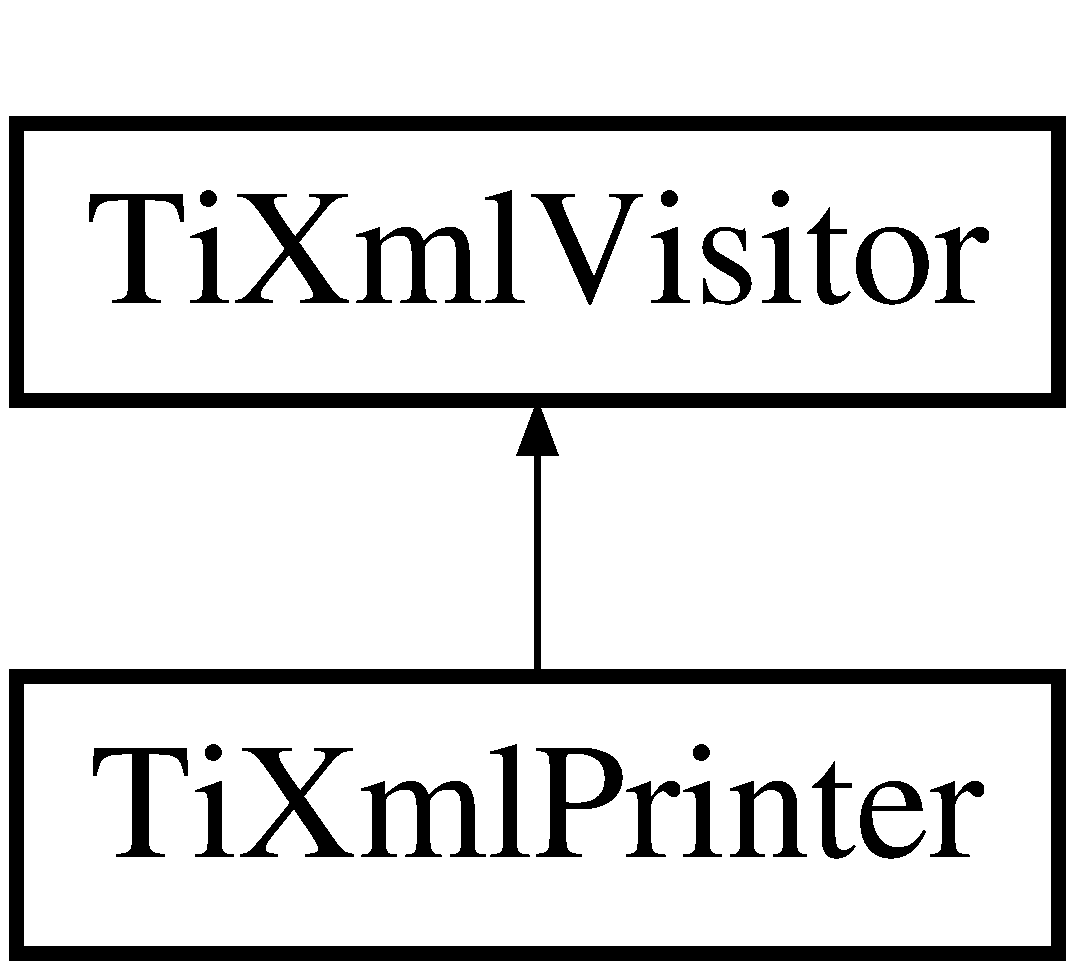
\includegraphics[height=2.000000cm]{class_ti_xml_visitor}
\end{center}
\end{figure}
\subsection*{Public Member Functions}
\begin{DoxyCompactItemize}
\item 
\hypertarget{class_ti_xml_visitor_a07baecb52dd7d8716ae2a48ad0956ee0}{virtual bool \hyperlink{class_ti_xml_visitor_a07baecb52dd7d8716ae2a48ad0956ee0}{Visit\+Enter} (const \hyperlink{class_ti_xml_document}{Ti\+Xml\+Document} \&)}\label{class_ti_xml_visitor_a07baecb52dd7d8716ae2a48ad0956ee0}

\begin{DoxyCompactList}\small\item\em Visit a document. \end{DoxyCompactList}\item 
\hypertarget{class_ti_xml_visitor_aa0ade4f27087447e93974e975c3246ad}{virtual bool \hyperlink{class_ti_xml_visitor_aa0ade4f27087447e93974e975c3246ad}{Visit\+Exit} (const \hyperlink{class_ti_xml_document}{Ti\+Xml\+Document} \&)}\label{class_ti_xml_visitor_aa0ade4f27087447e93974e975c3246ad}

\begin{DoxyCompactList}\small\item\em Visit a document. \end{DoxyCompactList}\item 
\hypertarget{class_ti_xml_visitor_af6c6178ffa517bbdba95d70490875fff}{virtual bool \hyperlink{class_ti_xml_visitor_af6c6178ffa517bbdba95d70490875fff}{Visit\+Enter} (const \hyperlink{class_ti_xml_element}{Ti\+Xml\+Element} \&, const \hyperlink{class_ti_xml_attribute}{Ti\+Xml\+Attribute} $\ast$)}\label{class_ti_xml_visitor_af6c6178ffa517bbdba95d70490875fff}

\begin{DoxyCompactList}\small\item\em Visit an element. \end{DoxyCompactList}\item 
\hypertarget{class_ti_xml_visitor_aec2b1f8116226d52f3a1b95dafd3a32c}{virtual bool \hyperlink{class_ti_xml_visitor_aec2b1f8116226d52f3a1b95dafd3a32c}{Visit\+Exit} (const \hyperlink{class_ti_xml_element}{Ti\+Xml\+Element} \&)}\label{class_ti_xml_visitor_aec2b1f8116226d52f3a1b95dafd3a32c}

\begin{DoxyCompactList}\small\item\em Visit an element. \end{DoxyCompactList}\item 
\hypertarget{class_ti_xml_visitor_afad71c71ce6473fb9b4b64cd92de4a19}{virtual bool \hyperlink{class_ti_xml_visitor_afad71c71ce6473fb9b4b64cd92de4a19}{Visit} (const \hyperlink{class_ti_xml_declaration}{Ti\+Xml\+Declaration} \&)}\label{class_ti_xml_visitor_afad71c71ce6473fb9b4b64cd92de4a19}

\begin{DoxyCompactList}\small\item\em Visit a declaration. \end{DoxyCompactList}\item 
\hypertarget{class_ti_xml_visitor_a399b8ebca5cd14664974a32d2ce029e5}{virtual bool \hyperlink{class_ti_xml_visitor_a399b8ebca5cd14664974a32d2ce029e5}{Visit} (const \hyperlink{class_ti_xml_text}{Ti\+Xml\+Text} \&)}\label{class_ti_xml_visitor_a399b8ebca5cd14664974a32d2ce029e5}

\begin{DoxyCompactList}\small\item\em Visit a text node. \end{DoxyCompactList}\item 
\hypertarget{class_ti_xml_visitor_a53a60e7a528627b31af3161972cc7fa2}{virtual bool \hyperlink{class_ti_xml_visitor_a53a60e7a528627b31af3161972cc7fa2}{Visit} (const \hyperlink{class_ti_xml_comment}{Ti\+Xml\+Comment} \&)}\label{class_ti_xml_visitor_a53a60e7a528627b31af3161972cc7fa2}

\begin{DoxyCompactList}\small\item\em Visit a comment node. \end{DoxyCompactList}\item 
\hypertarget{class_ti_xml_visitor_a7e284d607d275c51dac1adb58159ce28}{virtual bool \hyperlink{class_ti_xml_visitor_a7e284d607d275c51dac1adb58159ce28}{Visit} (const \hyperlink{class_ti_xml_unknown}{Ti\+Xml\+Unknown} \&)}\label{class_ti_xml_visitor_a7e284d607d275c51dac1adb58159ce28}

\begin{DoxyCompactList}\small\item\em Visit an unknown node. \end{DoxyCompactList}\end{DoxyCompactItemize}


\subsection{Detailed Description}
Implements the interface to the \char`\"{}\+Visitor pattern\char`\"{} (see the Accept() method.) If you call the Accept() method, it requires being passed a \hyperlink{class_ti_xml_visitor}{Ti\+Xml\+Visitor} class to handle callbacks. For nodes that contain other nodes (Document, Element) you will get called with a Visit\+Enter/\+Visit\+Exit pair. Nodes that are always leaves are simply called with \hyperlink{class_ti_xml_visitor_afad71c71ce6473fb9b4b64cd92de4a19}{Visit()}.

If you return 'true' from a Visit method, recursive parsing will continue. If you return false, {\bfseries no children of this node or its sibilings} will be Visited.

All flavors of Visit methods have a default implementation that returns 'true' (continue visiting). You need to only override methods that are interesting to you.

Generally Accept() is called on the \hyperlink{class_ti_xml_document}{Ti\+Xml\+Document}, although all nodes suppert Visiting.

You should never change the document from a callback.

\begin{DoxySeeAlso}{See also}
\hyperlink{class_ti_xml_node_acc0f88b7462c6cb73809d410a4f5bb86}{Ti\+Xml\+Node\+::\+Accept()} 
\end{DoxySeeAlso}


The documentation for this class was generated from the following file\+:\begin{DoxyCompactItemize}
\item 
C\+:/\+Users/\+Avenger/\+Documents/\+Git\+Hub/\+Projet-\/\+Tamagoshi/includes/tinyxml/tinyxml.\+h\end{DoxyCompactItemize}

\chapter{File Documentation}
\hypertarget{_disease_8h}{\section{C\+:/\+Users/\+Avenger/\+Documents/\+Git\+Hub/\+Projet-\/\+Tamagoshi/headers/\+Disease.h File Reference}
\label{_disease_8h}\index{C\+:/\+Users/\+Avenger/\+Documents/\+Git\+Hub/\+Projet-\/\+Tamagoshi/headers/\+Disease.\+h@{C\+:/\+Users/\+Avenger/\+Documents/\+Git\+Hub/\+Projet-\/\+Tamagoshi/headers/\+Disease.\+h}}
}


Header de la classe \hyperlink{class_disease}{Disease}.  


{\ttfamily \#include $<$iostream$>$}\\*
{\ttfamily \#include $<$string$>$}\\*
{\ttfamily \#include $<$stdlib.\+h$>$}\\*
{\ttfamily \#include $<$ctime$>$}\\*
\subsection*{Classes}
\begin{DoxyCompactItemize}
\item 
class \hyperlink{class_disease}{Disease}
\begin{DoxyCompactList}\small\item\em Classe qui repr�sente la maladie. \end{DoxyCompactList}\end{DoxyCompactItemize}


\subsection{Detailed Description}
Header de la classe \hyperlink{class_disease}{Disease}. 

\begin{DoxyAuthor}{Author}
Dupuy.\+N Roman.\+A Cartoux.\+T 
\end{DoxyAuthor}

%--- End generated contents ---

% Index
\newpage
\phantomsection
\addcontentsline{toc}{chapter}{Index}
\printindex

\end{document}
